\documentclass[a4paper,10pt,oneside,openany,fleqno]{article}
%%%%%%%%%%%%%%%%%%%%%%%%%%%%%%%%%%%%%%%%%%%%%%%%%%%%%%%%%%%%
\usepackage{pgf-PeriodicTable}
\usepgfPTlibrary{colorschemes}%
%%%%%%%%%%%%%%%%%%%%%%%%%%%%%%%%%%%%%%%%%%%%%%%%%%%%%%%%%%%%
% Definitions for pgf-PeriodicTable Manual
% Hugo Gomes @ 08/11/2022 v1.0.1
% Hugo Gomes @ 10/10/2022 v1.0.0
\def\pgfPTversion{2.0.0}%
\def\pgfPTnewinversion#1{new in v#1}%
\def\pgfPTchangedinversion#1{changed in v#1}%
%%%%%%%%%%%%%%%%%%%%%%%%%%%%%%%%%%%%%%%%%%%%%%%%%%%%%%%%%%%%
\usepackage[ansinew]{inputenc}
\usepackage{verdana}
%
\addtolength{\textwidth}{3.5cm}
\addtolength{\textheight}{2.5cm}
\addtolength{\topmargin}{-1.25cm}
\setlength{\parindent}{0pt}
\setlength{\oddsidemargin}{0pt}
\setcounter{secnumdepth}{1}%
\setcounter{tocdepth}{4}
%
%%%%%%%%%%%%%%%%%%%%%%%%%%%%%%%%%%%%%%%%%%%%%%%%%%%%%%%%%%%%
\pgfdeclarelayer{back}%
\pgfsetlayers{back,main}%
%%%%%%%%%%%%%%%%%%%%%%%%%%%%%%%%%%%%%%%%%%%%%%%%%%%%%%%%%%%%
\usetikzlibrary{shadows}%
%%%%%%%%%%%%%%%%%%%%%%%%%%%%%%%%%%%%%%%%%%%%%%%%%%%%%%%%%%%%
\usepackage{makeidx}
\makeindex%
% ------------------------------------------------------------------------------------------------------------------------------------
% BUILD SEQUENCE:
% 1) pdflatex.exe "pgf-PeriodicTableManual.tex"
% 2) makeindex.exe -s "pgf-PeriodicTableManual.ist" "pgf-PeriodicTableManual.idx"
% 3) pdflatex.exe "pgf-PeriodicTableManual.tex"
% ------------------------------------------------------------------------------------------------------------------------------------
\usepackage[skins]{tcolorbox}
\tcbuselibrary{breakable}
\usepackage[english]{babel}
\usepackage{pifont}
\usepackage[pdfstartview={ },colorlinks=true, linkcolor=black!50!green, citecolor=gray, urlcolor=teal, hyperindex, plainpages=false,bookmarksopenlevel=1,bookmarksopen=true]{hyperref}%
\hypersetup{%Start options on pdf
pdftitle = {Manual for pgf-PeriodicTable (v\pgfPTversion)},%
pdfsubject = {Periodic Table of Elements},%
pdfkeywords = {Draw the Periodic Table of Elements in a simple way via pgf/TikZ environment. It's possible to draw a full or partial Periodic Table of Elements},%
pdfauthor = {\textcopyright Hugo Gomes},%
pdfproducer = {pdfeTeX-1.\the\pdftexversion\pdftexrevision},
}%End options on pdf
\usepackage{fancyhdr}
\usepackage{lastpage}
\renewcommand{\headrulewidth}{0.4pt}%
\renewcommand{\footrulewidth}{0.4pt}%
\addtolength{\headheight}{25pt}%
\fancypagestyle{pgfPTManual}{%
\fancyhf{} % clear all header and footer fields
\fancyhead[R]{\usefont{T1}{vna}{m}{n}\nouppercase{\leftmark}}%
\fancyhead[L]{\color{blue!70!black}pgf-PeriodicTable \pgfPTversion}%
\fancyfoot[R]{\usefont{T1}{vna}{m}{n}\textbf{\thepage\ of \pageref{LastPage}}}%
\fancyfoot[L]{\ }}%
\fancypagestyle{plain}{%
\addtolength{\textwidth}{3.5cm}%
\fancyhf{} % clear all header and footer fields
\fancyhead[R]{\usefont{T1}{vna}{m}{n}\nouppercase{\leftmark}}%
\fancyhead[L]{\color{blue!70!black}pgf-PeriodicTable \pgfPTversion}%
\fancyfoot[R]{\usefont{T1}{vna}{m}{n}\textbf{\thepage\ of \pageref{LastPage}}}%
\fancyfoot[L]{\ }}%
\usepackage{amsfonts}
\usepackage{amssymb}
\usepackage{amsmath}
\usepackage{tabularx}
\usepackage{calc}
%%%%%%%%%%%%%%%%%%%%%%%%%%%%%%%%%%%%%%%%%%%%%%%%%%%%%%%%%%%%
\makeatletter%
\renewenvironment{theindex}%
               {\if@twocolumn%
                  \@restonecolfalse%
                \else%
                  \@restonecoltrue%
                \fi%
%             \twocolumn[\section*{\indexname}]%
                \twocolumn[\section{\indexname}]%
                \@mkboth{\MakeUppercase\indexname}%
                        {\MakeUppercase\indexname}%
                \thispagestyle{plain}\parindent\z@%
                \parskip\z@ \@plus .3\p@\relax%
                \columnseprule \z@%
                \columnsep 35\p@%
                \let\item\@idxitem}%
               {\if@restonecol\onecolumn\else\clearpage\fi}%
%%%%%%%%%%%%%%%%%%%%%%%%%%%%%%%%%%%%%%%%%%%%%%%%%%%%%%%%%%%%
\def\pack{\large\texttt{\color{blue!70!black}pgf-PeriodicTable}\normalsize}%
\def\txttt#1{\large\texttt{#1}\normalsize}%
\def\txttikz{{\fontfamily{cmr}\selectfont Ti\emph{k}Z}}%
\def\ie{\textit{i.e.\/}}%
\def\eg{\textit{e.g.\/}}%
\def\myldots{\tikz{\fill (0,0) circle(.6pt);\fill (2.4pt,0) circle(.6pt);\fill (4.8pt,0) circle(.6pt);}}%
\def\cyan#1{\textcolor{cyan!50!black}{#1}}%
\def\dcyan#1{\textcolor{cyan!30!black}{#1}}%
\def\gray#1{\textcolor{black!50}{#1}}%
\def\blue#1{\textcolor{blue!50!black}{#1}}%
\def\lblue#1{\textcolor{blue!70!black}{#1}}%
\def\green#1{\textcolor{green!50!black}{#1}}%
\def\red#1{\textcolor{red!50!black}{#1}}%
\def\orange#1{\textcolor{orange!80!black}{#1}}%
\def\bs#1{\textcolor{blue!50!black}{\textbackslash#1}}%
\def\lb{\textcolor{blue!50!black}{\{}}%
\def\rb{\textcolor{blue!50!black}{\}}}%
\def\lp{\textcolor{blue!50!black}{[}}%
\def\rp{\textcolor{blue!50!black}{]}}%
\def\fnt#1#2{\begingroup\fontfamily{#1}\selectfont#1\ -- #2\endgroup}%
\def\pgfPTM@quote{\tikz{\pgfmathparse{height("l")}\edef\@lht{\pgfmathresult}\draw[line width=.75pt,line cap=round] (0,0) (0,\@lht-.65pt) -- ++(0,-1.65pt);}}
\def\sq#1{\pgfPTM@quote\makebox[.875pt][s]{}\textcolor{green!50!black}{#1}\makebox[.875pt][s]{}\pgfPTM@quote}%
%%%%%%%%%%%%%%%%%%%%%%%%%%%%%%%%%%%%%%%%%%%%%%%%%%%%%%%%%%%%
\def\pgfPTMcolorDemo#1#2{\setbox0=\hbox{\makebox[23pt][s]{}#2}\vbox to 8pt{\hsize=\wd0\tikz{\draw[#1!50!black,fill=#1,rounded corners=2pt] (0,0) rectangle (20pt,8pt);\node[font=\small,right,inner sep=0pt] at (23pt,2.75pt) {#2};}}}%
\def\pgfPTMselectfont{\string\selectfont}%
\def\pgfPTMtiny{\string\tiny}%
\def\pgfPTMscriptsize{\string\scriptsize}%
\def\pgfPTMfootnotesize{\string\footnotesize}%
\def\pgfPTMsmall{\string\small}%
\def\pgfPTMlarge{\string\large}%
\def\pgfPTMLarge{\string\Large}%
\def\pgfPTMLARGE{\string\LARGE}%
\def\pgfPTMhuge{\string\huge}%
\def\pgfPTMHuge{\string\Huge}%
\def\pgfPTMitshape{\string\itshape}%
\def\pgfPTMbfseries{\string\bfseries}%
%%%%%%%%%%%%%%%%%%%%%%%%%%%%%%%%%%%%%%%%%%%%%%%%%%%%%%%%%%%%
\def\pgfPTMzerodepth#1{{\setbox0=\hbox{#1}\dp0=0pt\box0\relax}}%
\def\pgfPTMparbox#1{{\setbox0=\vbox{\parshape=2 0pt \linewidth 10pt \the\dimexpr \linewidth-10pt\relax{#1}}\usebox0\relax}}%
\def\pgfPTMline{\tikz{\fill[black!10,rounded corners=2pt] (0,0) rectangle (\linewidth,-4pt);}}%
%%%%%%%%%%%%%%%%%%%%%%%%%%%%%%%%%%%%%%%%%%%%%%%%%%%%%%%%%%%%
\newdimen\pgfPTMspace\pgfPTMspace=0pt%
% \pgfPTmacro{macro name}[options list]
\def\pgfPTMmacro#1[#2]{\ignorespaces%
\edef\pgfPTM@optionslist{#2}%
\ifx\pgfPTM@optionslist\@empty\relax\textcolor{blue!50!black}{\textbackslash #1}%
\else%
\textcolor{blue!50!black}{\textbackslash #1[}\textcolor{red!50!black}{\detokenize\expandafter{\pgfPTM@optionslist}}\textcolor{blue!50!black}{]}%
\fi%
}%
%%%%%%%%%%%%%%%%%%%%%%%%%%%%%%%%%%%%%%%%%%%%%%%%%%%%%%%%%%%%
% \pgfPTmacrobox[alignment]{macro name}[options list]
\def\pgfPTMmacrobox{\@ifnextchar[\pgfPTM@macrobox{\pgfPTM@macrobox[c]}}%
\def\pgfPTM@macrobox[#1]#2[#3]{\ignorespaces%
\edef\pgfPTM@optionslist{#3}%
\edef\pgfPTM@align{#1}\edef\pgfPTM@align@c{c}%
\ifx\pgfPTM@align\pgfPTM@align@c\relax\def\pgfPTM@alignment{flush center}\else\def\pgfPTM@alignment{left}\fi%
\ifx\pgfPTM@optionslist\@empty\relax%
\tikz{\node[text width=\linewidth-8pt,inner xsep=4pt,align=\pgfPTM@alignment,fill=black!10,rounded corners=2pt] %
{\textcolor{blue!50!black}{\textbackslash #2}};}%
\else%
\tikz{\node[text width=\linewidth-8pt,inner xsep=4pt,align=\pgfPTM@alignment,fill=black!10,rounded corners=2pt] %
{\textcolor{blue!50!black}{\textbackslash #2[}\textcolor{red!50!black}{\detokenize\expandafter{\pgfPTM@optionslist}}\textcolor{blue!50!black}{]}};}%
\fi%
}%
%%%%%%%%%%%%%%%%%%%%%%%%%%%%%%%%%%%%%%%%%%%%%%%%%%%%%%%%%%%%
\definecolor{cItemList}{rgb}{0.55,0.78,0.25}
\newenvironment{itemlist}{%
\begin{list}{\hfill$\boldsymbol{\checkmark}$}{\setlength{\parsep}{0pt}\setlength{\topsep}{4pt}\setlength{\leftmargin}{6mm}\setlength{\labelwidth}{1em}\setlength{\labelsep}{1pt}}}{\end{list}}
\tcolorboxenvironment{itemlist}{breakable,blanker,before skip=2pt,after skip=4pt,
                                                borderline west={2.8pt}{.75pt}{cItemList!75!black},
                                                borderline west={2.8pt}{3.55pt}{cItemList!75!black!50!white},
                                                borderline west={2.8pt}{6.35pt}{cItemList!25!white}}%
\newenvironment{itembar}{\footnotesize%
\begin{list}{\hfill$\boldsymbol{\checkmark}$}{\setlength{\parsep}{0pt}\setlength{\topsep}{4pt}\setlength{\leftmargin}{6mm}\setlength{\labelwidth}{1em}\setlength{\labelsep}{1pt}}}{\end{list}}
\tcolorboxenvironment{itembar}{breakable,blanker,before skip=6pt,after skip=6pt,
                                                borderline west={2.8pt}{.75pt}{blue!75!black},
                                                borderline west={2.8pt}{3.55pt}{blue!75!black!50!white},
                                                borderline west={2.8pt}{6.35pt}{blue!25!white}}%
\newtcbox{\use}{enhanced,nobeforeafter,tcbox raise base,boxrule=0.4pt,top=0mm,bottom=0mm,%
  right=0mm,left=15mm,arc=1pt,boxsep=2pt,%
  colframe=cyan!50!black,coltext=cyan!25!black,colback=cyan!10!white,fontupper=\scriptsize,%
  overlay={\begin{tcbclipinterior}\fill[cyan!50!white] (frame.south west)%
    rectangle node[text=white,font=\scriptsize\bfseries,anchor=mid] {USAGE:} ([xshift=15mm]frame.north west);\end{tcbclipinterior}}}
\newtcbox{\uselib}{enhanced,nobeforeafter,tcbox raise base,boxrule=0.4pt,top=0mm,bottom=0mm,%
  right=0mm,left=15mm,arc=1pt,boxsep=2pt,%
  colframe=cyan!50!black,coltext=cyan!25!black,colback=cyan!10!white,fontupper=\small,%
  overlay={\begin{tcbclipinterior}\fill[cyan!50!white] (frame.south west)%
    rectangle node[text=white,font=\small\bfseries,anchor=mid] {USAGE: } ([xshift=15mm]frame.north west);\end{tcbclipinterior}}}%
\newcommand\mymfbox[2][gray]{\begin{tcolorbox}
[breakable,enhanced,arc=2.5pt,outer arc=2.5pt,colback=#1!10!white,colframe=#1!50!black,boxsep=3pt,left=3pt,right=3pt,top=3pt,bottom=3pt,boxrule=1pt]
#2\end{tcolorbox}}
\def\mysmile{\tikz[scale=1.2]{\path[fill=yellow] (0,0) circle (.15cm);
                               \fill[black!90] (45:.9mm) circle (.175mm);
                               \fill[black!90] (135:.9mm) circle (.175mm);
                               \draw[line width=.15mm,black!90] (215:.9mm) arc (215:325:.9mm);}}
\newcommand\tcexemplo[2][EXEMPLO:]{\begin{tcolorbox}[breakable,enhanced,fonttitle=\bfseries,
                            colback=green!5!white,colframe=white!50!green,title=#1,after title={\hfill\mysmile},
                            ]
                            #2
                            \end{tcolorbox}}
%%%%%%%%%%%%%%%%%%%%%%%%%%%%%%%%%%%%%%%%%%%%%%%%%%%%%%%%%%%%
% \pgfPTMbuildcell(lines,columns)[entries]
\def\pgfPTMbuildcell(#1,#2)[#3]{\ignorespaces%
\tikz{\node[text width=\linewidth-8pt,inner xsep=4pt,align=left,fill=black!10,rounded corners=2pt] %
{\textcolor{blue!50!black}{\textbackslash pgfPTbuildcell(}\textcolor{red!50!black}{#1,#2}\textcolor{blue!50!black}{)}%
\textcolor{black!50}{\% #1\ rows by #2 columns}\\ \textcolor{blue!50!black}{[}%
\textcolor{red!50!black}{\detokenize\expandafter{#3}}\textcolor{blue!50!black}{]}};}%
}%
%%%%%%%%%%%%%%%%%%%%%%%%%%%%%%%%%%%%%%%%%%%%%%%%%%%%%%%%%%%%
% \pgfPTMbtn{txt}
\definecolor{btnBack}{RGB}{237,237,237}%
\definecolor{btnBorder}{RGB}{127,116,112}%
\def\pgfPTMbtn#1{\tikz[baseline=(X.base)]{\node[draw=btnBorder,fill=btnBack,rounded corners=1.5pt,inner sep=2pt,font=\small,text=black,anchor=base] (X) {\pgfPT@box@zerodepth{#1}};}}%
%%%%%%%%%%%%%%%%%%%%%%%%%%%%%%%%%%%%%%%%%%%%%%%%%%%%%%%%%%%%
% \pgfPTMbuildcellstyle{name}(lines,columns)[entries]
\def\pgfPTMbuildcellstyle#1(#2,#3)[#4]{\ignorespaces%
\tikz{\node[text width=\linewidth-8pt,inner xsep=4pt,align=left,fill=black!10,rounded corners=2pt] %
{\textcolor{blue!50!black}{\textbackslash pgfPTbuilcellstyle\{}\textcolor{red!50!black}{#1}\textcolor{blue!50!black}{\}}%
\textcolor{blue!50!black}{(}\textcolor{red!50!black}{#2,#3}\textcolor{blue!50!black}{)}%
\textcolor{black!50}{\% #2\ rows by #3 columns}\\ \textcolor{blue!50!black}{[}%
\textcolor{red!50!black}{\detokenize\expandafter{#4}}\textcolor{blue!50!black}{]}};}%
}%
%%%%%%%%%%%%%%%%%%%%%%%%%%%%%%%%%%%%%%%%%%%%%%%%%%%%%%%%%%%%
% \pgfPTMpreviewcellstyle[scale factor]{name}
\def\pgfPTMpreviewcellstyle[#1]#2{\ignorespaces%
\edef\pgfPTM@optionslist{#1}%
\ifx\pgfPTM@optionslist\@empty\relax%
\tikz{\node[text width=\linewidth-8pt,inner xsep=4pt,align=center,fill=black!10,rounded corners=2pt] %
{\textcolor{blue!50!black}{\textbackslash pgfPTpreviewcellstyle\{}\textcolor{red!50!black}{#2}\textcolor{blue!50!black}{\}}};}%
\else%
\tikz{\node[text width=\linewidth-8pt,inner xsep=4pt,align=center,fill=black!10,rounded corners=2pt] %
{\textcolor{blue!50!black}{\textbackslash pgfPTpreviewcellstyle[}\textcolor{red!50!black}{#1}\textcolor{blue!50!black}{]\{}%
\textcolor{red!50!black}{#2}\textcolor{blue!50!black}{\}}};}%
\fi%
}%
%%%%%%%%%%%%%%%%%%%%%%%%%%%%%%%%%%%%%%%%%%%%%%%%%%%%%%%%%%%%
% \pgfPTMpreviewcellstyle(line;column;what)(line_i to line_f)(column_i to column_f)
\def\pgfPTMcelldesign(#1;#2;#3)(#4 to #5)(#6 to #7){%
\makebox[\linewidth][c]{\begin{tikzpicture}
\draw[line width=1pt,fill=black!10] (0,0) rectangle ++(3,-4);
\foreach \x in {1,2}{\draw[dotted,line width=.8pt,red] (\x cm,0) node[above,xshift=-.5cm] {\x} -- ++(0,-4);}\node[red,above] at (2.5,0) {3};
\foreach \y in {1,...,4}{\draw[dotted,line width=.8pt,blue] (0,-.8*\y cm) node[left,yshift=.4cm] {\y} -- ++(3,0);}\node[blue,left] at (0,-3.6) {5};
\draw[line width=1pt,double distance=1pt,-stealth] (3.5,-2) -- ++(3,0) node[midway,above] {\green{(#1;#2;#3)}};
\draw[line width=1pt,fill=black!10] (7,0) rectangle ++(3,-4);
\foreach \x in {1,2}{\draw[dotted,line width=.8pt,red] (7cm+\x cm,0) node[above,xshift=-.5cm] {\x} -- ++(0,-4);}\node[red,above] at (9.5,0) {3};
\foreach \y in {1,...,4}{\draw[dotted,line width=.8pt,blue] (7cm,-.8*\y cm) node[left,yshift=.4cm] {\y} -- ++(3,0);}\node[blue,left] at (7,-3.6) {5};
\draw[green!50!black,fill=green!50!white,opacity=.5] (6cm+#6cm,-0.8*#4cm+.8cm) rectangle ++(#7cm-#6cm,-.8*#5cm+.8*#4cm) node[midway,opacity=1] {\green{#3}};
\end{tikzpicture}}}
%%%%%%%%%%%%%%%%%%%%%%%%%%%%%%%%%%%%%%%%%%%%%%%%%%%%%%%%%%%%
% \pgfPTMnewColorScheme[<trailing color (default=1/1/1 e.g. white)>]{name}{list}
\def\pgfPTMnewColorScheme[#1]#2#3{\ignorespaces%
\edef\pgfPTM@optionslist{#1}%
\ifx\pgfPTM@optionslist\@empty\relax%
\tikz{\node[text width=\linewidth-8pt,inner xsep=4pt,align=center,fill=black!10,rounded corners=2pt] %
{\textcolor{blue!50!black}{\textbackslash pgfPTnewColorScheme\{}\textcolor{red!50!black}{#2}\textcolor{blue!50!black}{\}\{}%
\textcolor{red!50!black}{#3}\textcolor{blue!50!black}{\}}};}%
\else%
\tikz{\node[text width=\linewidth-8pt,inner xsep=4pt,align=center,fill=black!10,rounded corners=2pt] %
{\textcolor{blue!50!black}{\textbackslash pgfPTnewColorScheme[}\textcolor{red!50!black}{#1}\textcolor{blue!50!black}{]\{}%
\textcolor{red!50!black}{#2}\textcolor{blue!50!black}{\}\{}%
\textcolor{red!50!black}{#3}\textcolor{blue!50!black}{\}}};}%
\fi%
}%
%%%%%%%%%%%%%%%%%%%%%%%%%%%%%%%%%%%%%%%%%%%%%%%%%%%%%%%%%%%%
% \pgfPTMnewZlist{name}{list}
\def\pgfPTMnewZlist#1#2{\ignorespaces%
\tikz{\node[text width=\linewidth-8pt,inner xsep=4pt,align=center,fill=black!10,rounded corners=2pt] %
{\textcolor{blue!50!black}{\textbackslash pgfPTnewZlist\{}\textcolor{red!50!black}{#1}\textcolor{blue!50!black}{\}\{}%
\textcolor{red!50!black}{#2}\textcolor{blue!50!black}{\}}};}%
}%
%%%%%%%%%%%%%%%%%%%%%%%%%%%%%%%%%%%%%%%%%%%%%%%%%%%%%%%%%%%%
% \pgfPTMsetLanguage{language flag}
\def\pgfPTMsetLanguage#1{\ignorespaces%
\tikz{\node[text width=\linewidth-8pt,inner xsep=4pt,align=center,fill=black!10,rounded corners=2pt] %
{\textcolor{blue!50!black}{\textbackslash pgfPTsetLanguage\{}\textcolor{red!50!black}{#1}\textcolor{blue!50!black}{\}}};}%
}%
%%%%%%%%%%%%%%%%%%%%%%%%%%%%%%%%%%%%%%%%%%%%%%%%%%%%%%%%%%%%%
% \pgfPTMoption[version]{level}{option}{default}{description} level=3-> subsubsection; level=4-> paragraph
\def\pgfPTMoption{\@ifnextchar[\pgfPTM@option{\pgfPTM@option[]}}%
\def\pgfPTM@option[#1]#2#3#4#5{\index{OPTIONS@\textbf{OPTIONS}!#3}\ignorespaces%
\ifnum#2=3\relax\vskip-4.75ex\vskip-18pt\ \subsubsection*{}\addcontentsline{toc}{subsubsection}{\texorpdfstring{$\rightsquigarrow$ #3}{#3}}%
\else\ifnum#2=4\relax\vskip-4.75ex\vskip-20pt\ \paragraph*{}\addcontentsline{toc}{paragraph}{\texorpdfstring{$\rightsquigarrow$ #3}{#3}}\ \\ [8pt]%
\fi\fi%
\edef\pgfPTM@version{#1}%
\begin{tikzpicture}%
\node[below right,font=\small\bfseries] (a) at (0,0) {\hypertarget{option:#3}{#3}};%
\node[below left,font=\small] (b) at (\textwidth-.3333em,0) {default: \itshape#4};%
\node[below right,text=black!80,font=\small,text width=\textwidth-.6666em] (c) at (a.south west) %
{#5\ifx\pgfPTM@version\@empty\relax\else\hfill\textit{\textcolor{blue}{(\pgfPTM@version)}}\fi};%
\begin{pgfonlayer}{back}%
\path[left color=orange!20,right color=black!20!orange!30,rounded corners=2pt] (a.north west) rectangle (c.south east);%
\end{pgfonlayer}%
\end{tikzpicture}%
}%
\def\pgfPTendoption{\\ [-6.75pt]\tikz{\path[left color=orange!20,right color=black!20!orange!30,rounded corners=2pt] (0,0) rectangle ++(\textwidth,-4.5pt);}}%
% \pgfPTMoptiontxt{description}
\def\pgfPTMoptiontxt#1{%
\begin{tikzpicture}%
\node[below right,text=black!80,font=\small,text width=\textwidth-.6666em] (a) at (0,0) {#1};%
\begin{pgfonlayer}{back}%
\path[draw=orange,left color=orange!10,right color=black!5!orange!15,rounded corners=2pt] (a.north west) rectangle (a.south east);%
\end{pgfonlayer}%
\end{tikzpicture}%
}%
%%%%%%%%%%%%%%%%%%%%%%%%%%%%%%%%%%%%%%%%%%%%%%%%%%%%%%%%%%%%%
% \pgfPTMstyle[version]{level}{style}{default}{description} level=3-> subsubsection; level=4-> paragraph
\def\pgfPTMstyle{\@ifnextchar[\pgfPTM@style{\pgfPTM@style[]}}%
\def\pgfPTM@style[#1]#2#3#4#5{\index{STYLES@\textbf{STYLES}!#3}\ignorespaces%
\ifnum#2=3\relax\vskip-4.75ex\vskip-18pt\ \subsubsection*{}\addcontentsline{toc}{subsubsection}{\texorpdfstring{\hspace{0.73003pt}\ding{252}\ #3}{#3}}%
\else\ifnum#2=4\relax\vskip-4.75ex\vskip-20pt\ \paragraph*{}\addcontentsline{toc}{paragraph}{\texorpdfstring{\hspace{0.73003pt}\ding{252}\ #3}{#3}}\ \\ [8pt]%
\fi\fi%
\edef\pgfPTM@version{#1}%
\begin{tikzpicture}%
\node[below right,font=\small\bfseries] (a) at (0,0) {\hypertarget{style:#3}{#3}};%
\node[below left,font=\small] (b) at (\textwidth-.3333em,0) {default: \itshape#4};%
\node[below right,text=black!80,font=\small,text width=\textwidth-.6666em] (c) at (a.south west) %
{#5\ifx\pgfPTM@version\@empty\relax\else\hfill\textit{\textcolor{blue}{(\pgfPTM@version)}}\fi};%
\begin{pgfonlayer}{back}%
\path[left color=cyan!20,right color=black!20!cyan!30,rounded corners=2pt] (a.north west) rectangle (c.south east);%
\end{pgfonlayer}%
\end{tikzpicture}%
}%
% \pgfPTMstyletxt[version]{level}{style}{txt}{description} level=3-> subsubsection; level=4-> paragraph
\def\pgfPTMstyletxt{\@ifnextchar[\pgfPTM@styletxt{\pgfPTM@styletxt[]}}%
\def\pgfPTM@styletxt[#1]#2#3#4#5{\index{STYLES@\textbf{STYLES}!#3}\ignorespaces%
\ifnum#2=3\relax\vskip-4.75ex\vskip-18pt\ \subsubsection*{}\addcontentsline{toc}{subsubsection}{\texorpdfstring{\hspace{0.73003pt}\ding{252}\ #3}{#3}}%
\else\ifnum#2=4\relax\vskip-4.75ex\vskip-20pt\ \paragraph*{}\addcontentsline{toc}{paragraph}{\texorpdfstring{\hspace{0.73003pt}\ding{252}\ #3}{#3}}\ \\ [8pt]%
\fi\fi%
\edef\pgfPTM@version{#1}%
\begin{tikzpicture}%
\node[below right,font=\small\bfseries] (a) at (0,0) {\hypertarget{option:#3}{#3}};%
\node[below left,font=\small] (b) at (\textwidth-.3333em,0) {\itshape#4};%
\node[below right,text=black!80,font=\small,text width=\textwidth-.6666em] (c) at (a.south west) %
{#5\ifx\pgfPTM@version\@empty\relax\else\hfill\textit{\textcolor{blue}{(\pgfPTM@version)}}\fi};%
\begin{pgfonlayer}{back}%
\path[left color=cyan!20,right color=black!20!cyan!30,rounded corners=2pt] (a.north west) rectangle (c.south east);%
\end{pgfonlayer}%
\end{tikzpicture}%
}%
\def\pgfPTendstyle{\\ [-6.75pt]\tikz{\path[left color=cyan!20,right color=black!20!cyan!30,rounded corners=2pt] (0,0) rectangle ++(\textwidth,-4.5pt);}}%
% \pgfPTMoptiontxt{description}
%%%%%%%%%%%%%%%%%%%%%%%%%%%%%%%%%%%%%%%%%%%%%%%%%%%%%%%%%%%%
% for data table
\newdimen\cellht%
\newdimen\wdbi\newdimen\wdbii\newdimen\wdbiii\newdimen\wdbiv%
\newdimen\boxinnersep\boxinnersep=16pt\relax%
%
\def\header{%
\wdbi=.125\linewidth\wdbii=.2\linewidth\wdbiii=.2\linewidth\wdbiv=.475\linewidth%

\begin{tikzpicture}[every node/.style={inner sep=0pt,font=\scriptsize\bfseries,fill=black!30,below right,text height=10pt,text depth=4pt,text=white,draw=black!30}]
\node[text width=\wdbi] (acron) at (0,0) {\ acronym};% 1
\node[text width=\wdbii] (desc) at ([xshift=-1pt]acron.north east) {\ description};% 2
\node[text width=\wdbiii] (unit) at ([xshift=-1pt]desc.north east) {\ unit};% 3
\node[text width=\wdbiv] at ([xshift=-1pt]unit.north east) {\ remarks (compiled from @date)};% 4
\end{tikzpicture}%
}%
\def\linhaimpar#1#2#3#4{%
\@linha{#1}{#2}{#3}{#4}[black!5]
}%
\def\linhapar#1#2#3#4{%
\@linha{#1}{#2}{#3}{#4}[black!10]
}%
\def\@linha#1#2#3#4[#5]{%
\wdbi=.125\linewidth\wdbii=.2\linewidth\wdbiii=.2\linewidth\wdbiv=.475\linewidth%
\advance\wdbi  by-\boxinnersep\relax%
\advance\wdbii  by-\boxinnersep\relax%
\advance\wdbiii  by-\boxinnersep\relax%
\advance\wdbiv  by-\boxinnersep\relax%
\setbox0=\vbox{\hsize=\wdbi\scriptsize#1}%
\setbox1=\vbox{\hsize=\wdbii\scriptsize#2}%
\setbox2=\vbox{\hsize=\wdbiii\scriptsize#3}%
\setbox3=\vbox{\hsize=\wdbiv\scriptsize#4}%
\cellht=\ht0\relax%
\ifdim\cellht<\ht1\relax\cellht=\ht1\relax\fi%
\ifdim\cellht<\ht2\relax\cellht=\ht2\relax\fi%
\ifdim\cellht<\ht3\relax\cellht=\ht3\relax\fi%
\setbox0=\vbox to \cellht{\hsize=\wdbi\scriptsize#1\vfill}%
\setbox1=\vbox to \cellht{\hsize=\wdbii\scriptsize#2\vfill}%
\setbox2=\vbox to \cellht{\hsize=\wdbiii\scriptsize#3\vfill}%
\setbox3=\vbox to \cellht{\hsize=\wdbiv\scriptsize#4\vfill}%
\begin{tikzpicture}[every node/.style={inner xsep=.225\boxinnersep,draw=black!75,fill=#5,below right,text height=\cellht,text depth=2pt}]
\node[text width=\wdbi+.55\boxinnersep] (acron) at (0,0) {\color{red!50!black}\usebox0};
\node[text width=\wdbii+.55\boxinnersep] (desc) at ([xshift=-1pt]acron.north east) {\usebox1};
\node[text width=\wdbiii+.55\boxinnersep] (unit) at ([xshift=-1pt]desc.north east) {\usebox2};
\node[text width=\wdbiv+.55\boxinnersep] at ([xshift=-1pt]unit.north east) {\usebox3};
\end{tikzpicture}%
}%
%%%%%%%%%%%%%%%%%%%%%%%%%%%%%%%%%%%%%%%%%%%%%%%%%%%%%%%%%%%%%%%%%%%%%%%
% LIBRARIES
%%%%%%%%%%%%%%%%%%%%%%%%%%%%%%%%%%%%%%%%%%%%%%%%%%%%%%%%%%%%%%%%%%%%%%%
\def\pgfPTlib#1#2{\begingroup\renewcommand{\hrulefill}{\leavevmode\leaders\hrule height 1pt\hfill\kern0pt}%
\renewcommand{\dotfill}{\leavevmode\cleaders\hbox to 1.0em{\hss --\hss }\hfill\kern0pt}%
\setbox0=\hbox{\ pgf-PeriodicTable Library \red{\hypertarget{lib:#1}{#1}}\ }%
\raisebox{.25\ht0}{\makebox[.1125\linewidth][s]{\color{cyan!50!black}\hrulefill}}%
\hspace{-.1125\linewidth}\raisebox{.25\ht0+1.75pt}{\makebox[.1125\linewidth][s]{\color{cyan!70!black}\hrulefill}}%
\usebox0%
\raisebox{.25\ht0}{\makebox[.8875\linewidth-\wd0][s]{\color{cyan!50!black}\hrulefill}}%
\hspace{-.8875\linewidth}\hspace{\wd0}\raisebox{.25\ht0+1.75pt}{\makebox[.8875\linewidth-\wd0][s]{\color{cyan!70!black}\hrulefill}}%
\\ [12pt]\makebox[8pt][s]{}\uselib{\bs{usepgfPTlibrary}\lb\red{#1}\rb}%
\\ [12pt]\makebox[\linewidth][s]{\color{cyan!50!black}\dotfill}%
\\ [6pt]\makebox[8pt][s]{}\begin{minipage}{\linewidth-16pt}#2\end{minipage}%
\\ [6pt]\makebox[\linewidth][s]{\color{cyan!70!black}\hrulefill}\hspace{-\linewidth}%
\raisebox{1.75pt}{\makebox[\linewidth][s]{\color{cyan!50!black}\hrulefill}}\endgroup%
}%
%%%%%%%%%%%%%%%%%%%%%%%%%%%%%%%%%%%%%%%%%%%%%%%%%%%%%%%%%%%%
\def\pgfPTMlibsubsubsection#1{%
\tikz{\node[cyan!50!black,font=\large] (ding) at (0,0) {\ding{224} };%
\node[fill=cyan!5!white,text width={\linewidth-14.68799pt-1em},below right] (txt) at ([yshift=1pt]ding.north east) {#1};%
\draw[cyan!50!black] (txt.north west) -- (txt.north east);%
\draw[cyan!50!black] (txt.south west) -- (txt.south east);%
}}%
%%%%%%%%%%%%%%%%%%%%%%%%%%%%%%%%%%%%%%%%%%%%%%%%%%%%%%%%%%%%
% \pgfPTMlibexample{codetxt}{code}
\def\pgfPTMlibexample#1#2{\ignorespaces%
\begin{tikzpicture}%
\node[below right,text width=\textwidth-.6666em,rounded corners=2pt,left color=black!10,right color=black!14] (a) at (0,0) {#1};%
\node[below right,text width=\textwidth-.6666em,text centered] (c) at (a.south west) {#2};%
\begin{pgfonlayer}{back}%
%\path[left color=black!5!cyan!12,right color=teal!12!white,draw=cyan!50!black,rounded corners=2pt] (a.north west) rectangle (c.south east);%
\path[left color=white,right color=cyan!4,draw=cyan!50!black,rounded corners=2pt] (a.north west) rectangle (c.south east);%
\end{pgfonlayer}%
\end{tikzpicture}%
}%
\makeatother%
%
\endinput%

%%%%%%%%%%%%%%%%%%%%%%%%%%%%%%%%%%%%%%%%%%%%%%%%%%%%%%%%%%%%
\title{Manual for pgf-PeriodicTable \pgfPTversion}
\author{Hugo Gomes\\
  \texttt{hugo.parelho@gmail.com}}
\date{\today}
%%%%%%%%%%%%%%%%%%%%%%%%%%%%%%%%%%%%%%%%%%%%%%%%%%%%%%%%%%%%
\begin{document}%
\begin{titlepage}
\vspace{\stretch{1}}%
\maketitle\thispagestyle{empty}%
\vspace{-1cm}%
\makebox[\linewidth][c]{\scalebox{.6}{\pgfPT[show title=false,show legend=false]}}%
\\ [6pt]\makebox[\linewidth][c]{\bfseries\footnotesize\textsf{\pgfPTMmacro{pgfPT}[show title=false,show legend=false]}}%
\vspace{\stretch{6}}
\makebox[\linewidth][c]{\tikz{%
\node[text width=.9\linewidth+.5cm,text justified,draw=blue!10!black,rounded corners=10pt,fill=blue!5] at (0,0) {\color{blue!10!black}
\begin{abstract}
\noindent The purpose of this package is to provide the Periodic Table of Elements in a simple way. It relies on pgf/\txttikz{} to offer a full or partial periodic table with a variety of options and displaying the desired data. The data available, from all the actual 118 elements, is: atomic number, element name, chemical symbol, relative atomic mass, standard relative atomic mass, radioactivity, atomic radius (empirycal), covalente radius, ionic radius, first ionization energy, electronegati\-vity (Pauling), electroaffinity, oxidation states, melting point (in Kelvin and Celsius degrees), boiling point (in Kelvin and Celsius degrees), electron distribuition, electronic configuration (increasing $n$ and increasing $n+\ell$), density, specific heat capacity, thermal condutivity, lattice structure, lattice constants (a, b, c and c/a ratio), discovery year, discovery country and visible range spectral lines. It is possible to get the Periodic Table in six languages: English, French, German, Portuguese (from Portugal and from Brazil), Spanish and Italian.
\\ [6pt]
\end{abstract}
};}}
\vspace{\stretch{3}}
\end{titlepage}
\newpage%
%%%%%%%%%%%%%%%%%%%%%%%%%%%%%%%%%%%%%%%%%%%%%%%%%%%%%%%%%%%%
\pagestyle{empty}%
\pdfbookmark[1]{Table of contents}{pdfContents}%
\tableofcontents%
%%%%%%%%%%%%%%%%%%%%%%%%%%%%%%%%%%%%%%%%%%%%%%%%%%%%%%%%%%%%
\newpage\setcounter{page}{1}%
\pagestyle{pgfPTManual}%
\ \vfill%
\section{Installation and usage}
\noindent
\pack{} is placed under the terms of the \textrm{\LaTeX} Project Public License, version 1.3 or later (http://www.latex-project.org/lppl.txt). \pack{} loads and only requires the \href{https://www.ctan.org/pkg/pgf}{\txttikz{}} package.
\\ [6pt]You need to put the package files (pgf-PeriodicTable.sty \&\ \textit{friends}) in a location where \textrm{PDF\LaTeX}, \textrm{Lua\LaTeX} or \textrm{Xe\LaTeX} can find them. According to the TDS conventions this may be a subdirectory named \textit{tex/latex/pgf-PeriodicTable/} or \textit{tex/latex/misc/} in your (site specific) installation tree (insert your appropriate directory delimiter instead of /, if needed).
\\ [6pt]If you are using \textrm{PDF\LaTeX}, \textrm{Lua\LaTeX} or \textrm{Xe\LaTeX} you can just simply include the style file without any option via the \texttt{\large\textcolor{green!40!black}{\textbackslash usepackage}} command, \texttt{\large\textcolor{green!40!black}{\textbackslash usepackage}\textcolor{purple!70!black}{\{}\textcolor{blue!70!black}{pgf-PeriodicTable}\textcolor{purple!40!black}{\}}}
\\ [6pt]It can also be loaded with \textit{one option} to select the desired language:\\ \texttt{\large\textcolor{green!40!black}{\textbackslash usepackage}\textcolor{blue!70!black}{[}\textcolor{brown!60!black}{language flag}\textcolor{blue!70!black}{]}\textcolor{purple!70!black}{\{}\textcolor{blue!70!black}{pgf-PeriodicTable}\textcolor{purple!40!black}{\}}}
\\ [6pt]\textit{The \textcolor{brown!60!black}{language flags} available are:}
\begin{itemize}
\item[$\checkmark$]\textbf{en} for English (default),
\item[$\checkmark$]\textbf{fr} for French,
\item[$\checkmark$]\textbf{de} for German,
\item[$\checkmark$]\textbf{pt} for Portuguese (Portugal),
\item[$\checkmark$]\textbf{br} for Portuguese (Brazil),
\item[$\checkmark$]\textbf{es} for Spanish and
\item[$\checkmark$]\textbf{it} for Italian.
\end{itemize}
\vfill\vfill\vfill\newpage\ \vfill%
\section{The data}
The data available in \pack{} was mainly compiled with selected and filtered data from Wikipedia, taken from November 2021 to July 2022.
\\ [12pt]\header
\\ [-1pt]\linhaimpar{Ar}{Relative Atomic Mass}{}{(Wikidata @09/jan/2022)}%
\\ [-1pt]\linhapar{Arstar}{Standard Relative\newline Atomic Mass}{}{ STANDARD ATOMIC WEIGHTS 2021, %
Commission on Isotopic Abundances and Atomic Weights,\newline\bfseries\textsf{\textcopyright} CIAAW, 2007--2022%
\newline(\href{https://ciaaw.org/impressum.htm}{https://ciaaw.org/impressum.htm})}%
\\ [-1pt]\linhaimpar{radio}{Radioactivity}{}{(gperiodic-3.0.3, Dec 26 2018)}%
\\ [-1pt]\linhapar{R}{Atomic Radius}{$\mathsf{pm}$}{Calculated (Wikidata @04/jul/2022)}%
\\ [-1pt]\linhaimpar{Rcov}{Covalente Radius}{$\mathsf{pm}$}{Single bond, Wikidata @04/jul/2022)}%
\\ [-1pt]\linhapar{Rion}{Ionic Radius}{$\mathsf{pm}$}{(Wikidata @04/jul/2022)}%
\\ [-1pt]\linhaimpar{Ei}{First Ionization Energy}{$\mathsf{kJ\cdot mol^{-1}}$}{(Wikidata @04/jul/2022)}%
\\ [-1pt]\linhapar{eneg}{Electronegativity\newline (Pauling)}{}{(Wikidata @04/jul/2022)}%
\\ [-1pt]\linhaimpar{eaff}{Electroaffinity}{$\mathsf{kJ\cdot mol^{-1}}$}{(Wikidata @04/jul/2022)}%
\\ [-1pt]\linhapar{O}{Oxidation States}{}{(Wikidata @09/jan/2022)}%
\\ [-1pt]\linhaimpar{Tmelt}{Melting Point}{$\mathsf{K}$}{at standard pressure (Wikidata @21/dez/2021)}%
\\ [-1pt]\linhapar{TmeltC}{Melting Point}{$\mathsf{^oC}$}{at standard pressure (Wikidata @21/dez/2021)}%
\\ [-1pt]\linhaimpar{Tboil}{Boiling Point}{$\mathsf{K}$}{at standard pressure (Wikidata @21/dez/2021)}%
\\ [-1pt]\linhapar{TboilC}{Boiling Point}{$\mathsf{^oC}$}{at standard pressure (Wikidata @21/dez/2021)}%
\\ [-1pt]\linhaimpar{eDist}{Electron Distribution}{}{(Wikidata @01/nov/2021)}%
\\ [-1pt]\linhapar{eConfign}{Electronic Configuration (increasing n)}{}{(Wikidata @01/nov/2021)}%
\\ [-1pt]\linhaimpar{eConfign}{Electronic Configuration (increasing $\mathsf{n+\ell}$)}{}{(Wikidata @01/nov/2021)}%
\\ [-1pt]\linhapar{d}{Density}{$\mathsf{g\cdot dm^{-3}}$ {\tiny for gases}\newline$\mathsf{g\cdot cm^{-3}}$ {\tiny all other physical states}}{physical state at $\mathsf{25^oC, 1\,atm}$ (Wikidata @01/nov/2021)}%
\\ [-1pt]\linhaimpar{Cp}{Specific heat capacity}{$\mathsf{J\cdot mol^{-1}\cdot K^{-1}}$}{at $\mathsf{25^oC}$ and $\mathsf{100\,kPa}$ (Wikidata @20/nov/2021)}%
\\ [-1pt]\linhapar{kT}{Thermal Conductivity}{$\mathsf{W\cdot m^{-1}\cdot K^{-1}}$}{at $\mathsf{25^oC}$ (Wikidata @21/nov/2021)}%
\\ [-1pt]\linhaimpar{ls}{Lattice Structure}{}{(Wikidata @20/dez/2021 and \href{http://wwwhomes.uni-bielefeld.de/achim/ele_structures.html}{University of Bielefeld})}%
\\ [-1pt]\linhapar{lsa}{Lattice constant: a}{$\mathsf{pm}$}{(University of Bielefeld @21/dez/2021)}%
\\ [-1pt]\linhaimpar{lsb}{Lattice constant: b}{$\mathsf{pm}$}{(University of Bielefeld @21/dez/2021)}%
\\ [-1pt]\linhapar{lsc}{Lattice constant: c}{$\mathsf{pm}$}{(University of Bielefeld @21/dez/2021)}%
\\ [-1pt]\linhaimpar{lsca}{Lattice c/a ratio}{}{Calculated from available data and rounded to two digits}%
\\ [-1pt]\linhapar{DiscY}{Discover Year}{}{(Wikidata @22/dez/2021)}%
\\ [-1pt]\linhaimpar{DiscC}{Discover Country}{}{(Wikidata @22/dez/2021)}%
\\ [-1pt]\linhapar{spectra}{Visible range spectral lines}{}{Elements spectrum made with \textcolor{blue!50!black}{\textbackslash pgfspectra}.\newline See the \footnotesize\href{https://ctan.org/pkg/pgf-spectra}{\textsf{pgf-spectra}}\scriptsize\ manual for more details}%
\\ [12pt]The utilization of the \textit{acronyms} will be explained in \hyperlink{secBuildCell}{Designing cells with \textbackslash pgfPTbuildcell}.
\vfill\vfill\vfill\newpage
%%%%%%%%%%%%%%%%%%%%%%%%%%%%%%%%%%%%%%%%%%%%%%%%%%%%%%%%%%%%
\label{file:commands}%
\section{The commands}
\hypertarget{sec:com}{The} commands to achieve the Periodic Table of Elements are:
\begin{itemize}
\item\pgfPTMmacro{pgfPT}[]\ or \pgfPTMmacro{pgfPT}[options list] -- draws a full or partial graphical Periodic Table controlled by the optional keys.
\item\pgfPTMmacro{pgfPTstyle}[options list] -- sets the global style for the Periodic Table.
\item\pgfPTMmacro{pgfPTresetstyle}[] -- resets the style for the Periodic Table with the default values.
\item\pgfPTMmacro{pgfPTbuildcell}[]\blue{(}\textcolor{red!50!black}{nrows,ncolumns}\blue{)}\lp\red{entries}\rp%
\ -- builds the contents of each cell in the Periodic Table.
\item\pgfPTMmacro{pgfPTresetcell}[] -- resets the cell to its default layout.%
\item\pgfPTMmacro{pgfPTbuildcellstyle}[]\lb\red{name}\rb\blue{(}\red{nrows,ncolumns}\blue{)}\lp\red{entries}\rp%
\ -- builds the contents of each cell in the Periodic Table and stores it in a named style.
%\item\pgfPTMmacro{showcellinfo}[] -- shows the information about the contents of the last unnamed builded cell. If no cells have yet been build, the default cell is shown.
%\item\pgfPTMmacro{showcellstyleinfo}[]\textcolor{blue!50!black}{(}\textcolor{red!50!black}{name}\textcolor{blue!50!black}{)} -- shows the information about the contents of the named builded cell.
\item\pgfPTMmacro{pgfPTpreviewcell}[]\ or \pgfPTMmacro{pgfPTpreviewcell}[scale factor] -- preview the last unnamed built cell with an optional scale factor. If no cells have yet been built, the default cell is shown.
\item\pgfPTMmacro{pgfPTpreviewcellstyle}[]\lb\red{name}\rb%
\ or \pgfPTMmacro{pgfPTpreviewcellstyle}[]\lp\red{scale factor}\rp\lb\red{name}\rb%
\ -- preview the named builded cell with an optional scale factor.
\item\pgfPTMmacro{pgfPTnewcolorscheme}[trailing color]\lb\red{name}\rb\lb\red{color list}\rb%
\ -- makes a color scheme to fill the cells along the Periodic Table.
\item\pgfPTMmacro{pgfPTnewZlist}[]\lb\red{name}\rb%
\ -- create a user defined atomic numbers (Z) \red{named} list.
\item\pgfPTMmacro{pgfPTsetLanguage}[]\lb\red{language flag}\rb%
\ -- globally change the default language.
\end{itemize}
\vspace{-32pt}\ %
\def\tmpSection{\bs{pgfPT}}%
\subsection*{}{\normalfont\large\bfseries\raisebox{1.25pt}{$\mathbf{\blacktriangleright}$}\ Utilization of \tmpSection}%
\label{command:pgfPT}\addcontentsline{toc}{subsection}{\texorpdfstring{\tmpSection{}}{\textbackslash pgfPT}}%
\index{COMMANDS@\textbf{COMMANDS}!\textbackslash pgfPT}%
\\ [4pt]Use this command to draw the Periodic Table of Elements in the language selected at package inclusion (\texttt{\large\textcolor{green!40!black}{\textbackslash usepackage}\textcolor{blue!70!black}{[}\textcolor{brown!60!black}{language flag}\textcolor{blue!70!black}{]}\textcolor{purple!70!black}{\{}\textcolor{blue!70!black}{pgf-PeriodicTable}\textcolor{purple!40!black}{\}}}):
\\ [5pt]\pgfPTMmacrobox{pgfPT}[]%
\\ [10pt]\makebox[\linewidth][c]{\scalebox{.6}{\pgfPT}}%
\\ [0pt]\pgfPTMline%
\newpage%
This command can also be used with options -- as described in section \hyperlink{OPTIONS}{Options for \textbackslash pgfPT: creating a �Periodic Table�} -- to modify, for instance, the font of the Periodic Table or the colors of the cells:
\\ [10pt]\pgfPTMmacrobox{pgfPT}[font=pnc,back color scheme=MNM]%
\\ [10pt]\makebox[\linewidth][c]{\scalebox{.6}{\pgfPT[font=pnc,back color scheme=MNM]}}%
\\ [0pt]\pgfPTMline%
%%%%%%%%%%%%%%%%%%%%%%%%%%%%%%%%%%%%%%%%%%%%%%%%%%%%%%%%%%%%
\\ [-32pt]\ %
\def\tmpSection{\bs{pgfPTstyle}\lp\red{options list}\rp}%
\subsection*{}{\normalfont\large\bfseries\raisebox{1.25pt}{$\mathbf{\blacktriangleright}$}\ Utilization of \tmpSection}%
\label{command:pgfPTstyle}\addcontentsline{toc}{subsection}{\texorpdfstring{\tmpSection{}}{\textbackslash pgfPTstyle}}%
\index{COMMANDS@\textbf{COMMANDS}!\textbackslash pgfPTstyle}%
\\ [4pt]This command globally sets a style for the Periodic Table:
\\ [10pt]\pgfPTMmacrobox[l]{pgfPTstyle}[font=ptm,IUPAC=false,show title=false]%
\pgfPTstyle[font=ptm,IUPAC=false,show title=false]%
\\ [-4pt]\pgfPTMmacrobox{pgfPT}[]%
\\ [10pt]\makebox[\linewidth][c]{\scalebox{.6}{\pgfPT}}%
\\ [0pt]\pgfPTMline%
\newpage%\\ [5pt]
It is possible to locally override the \textit{global style} defined:
\\ [5pt]\pgfPTMmacrobox{pgfPT}[show title]%
\\ [10pt]\makebox[\linewidth][c]{\scalebox{.6}{\pgfPT[show title]}}%
\\ [5pt]\pgfPTMline%
%%%%%%%%%%%%%%%%%%%%%%%%%%%%%%%%%%%%%%%%%%%%%%%%%%%%%%%%%%%%
%\newpage\ \\ [-62pt]%
\\ [-32pt]\ %
\def\tmpSection{\bs{pgfPTresetstyle}}%
\subsection*{}{\normalfont\large\bfseries\raisebox{1.25pt}{$\mathbf{\blacktriangleright}$}\ Utilization of \tmpSection}%
\label{command:pgfPTresetstyle}\addcontentsline{toc}{subsection}{\texorpdfstring{\tmpSection{}}{\textbackslash pgfPTresetstyle}}%
\index{COMMANDS@\textbf{COMMANDS}!\textbackslash pgfPTresetstyle}%
\\ [4pt]This command resets the style used in the Periodic Table to default values:
\\ [10pt]\pgfPTMmacrobox[l]{pgfPTresetstyle}[]%
\pgfPTresetstyle%
\\ [-4pt]\pgfPTMmacrobox{pgfPT}[]%
\\ [10pt]\makebox[\linewidth][c]{\scalebox{.6}{\pgfPT}}%
\\ [0pt]\pgfPTMline%
%%%%%%%%%%%%%%%%%%%%%%%%%%%%%%%%%%%%%%%%%%%%%%%%%%%%%%%%%%%%
\newpage\ \\ [-62pt]
%\\ [-32pt]\ %
\def\tmpSection{\bs{pgfPTbuildcell}\blue{(}\red{nrows,ncolumns}\blue{)}\lp\red{entries}\rp}%
\subsection*{}{\color{black}\normalfont\large\bfseries\raisebox{1.25pt}{$\mathbf{\blacktriangleright}$}\ Utilization of \tmpSection}%
\label{command:pgfPTbuildcell}\addcontentsline{toc}{subsection}{\texorpdfstring{\tmpSection{}}{\textbackslash pgfPTbuildcell}}%
\index{COMMANDS@\textbf{COMMANDS}!\textbackslash pgfPTbuildcell}%
\\ [4pt]With \pgfPTMmacro{pgfPTbuildcell}[] it is possible to customize the \textit{elementar} cell of the Periodic Table. Each cell is built on the given \textit{number of rows} and \textit{number of columns}. After that, each \textit{entry} is constructed according to the structure \red{row;column;what} or \red{initial row-final row;initial column-final column;what}.
\vspace{8pt}%
\begin{itemlist}
\item The first \textit{syntax} -- \red{row;column;what} -- puts �\red{what}� in the �\red{row}� row and in the �\red{column}� column with the height of one row and the width of one column:
\\ -- for example, \red{1;1;Z} puts the atomic number \red{Z} in row \red{1} and column \red{1}, witch actually corresponds to a box anchored to the top left corner of the cell and that \textit{goes} below and to the right of that corner.
\item The second \textit{syntax} -- \mbox{\red{initial row-final row;initial column-final column;what}} -- puts �\red{what}� from �\red{initial row}� to �\red{final row}� with the height of $\textsf{\large final row}-\textsf{\large initial row}+\textsf{1}$ and from �\red{initial column}� to �\red{final column}� with the width of $\textsf{\large final column}-\textsf{\large initial column}+\textsf{1}$. It is important to keep in mind that when using this syntax the \textit{row} and \textit{column} could have any value between \textbf{1} and \textbf{number of rows} and \textbf{number of columns}, respectively.
\\ -- for example, \red{1;1-2.1;Z} puts the atomic number \red{Z} in row \red{1} with the height of one row and from column \red{1} to \textit{column} \red{2\mbox{.}1}, with the width of $\textsf{2\mbox{.}1}\times\textsf{\large column}$. Note that in this example the two \textit{syntaxes} are mixed up.
\end{itemlist}
\vspace{8pt}The \textbf{default cell} of the Periodic Table is constructed with the command:
\\ [10pt]\pgfPTMbuildcell(5,3)[(1;1-2;Z),(1;3;radio),(2-3;1.5-2.5;CS),(4;1-3;name),(5;1-3;Ar)]
%%%%%%%%%%%%%%%%%%%%%%%%%%%%%%%%%%%%%%%%%%%%%%%%%%%%%%%%%%%%
\\ [-32pt]\ %
\def\tmpSection{\bs{pgfPTresetcell}}%
\subsection*{}{\normalfont\large\bfseries\raisebox{1.25pt}{\color{black}$\mathbf{\blacktriangleright}$}\ Utilization of \tmpSection}%
\label{command:pgfPTresetcell}\addcontentsline{toc}{subsection}{\texorpdfstring{\tmpSection{}}{\textbackslash pgfPTbuildcellstyle}}%
\index{COMMANDS@\textbf{COMMANDS}!\textbackslash pgfPTresetcell}%
\\ [4pt]The \pgfPTMmacro{pgfPTresetcell}[] resets the cell to its default layout.
\\ [-32pt]\ %
\def\tmpSection{\bs{pgfPTbuildcellstyle}\lb\red{name}\rb\blue{(}\red{nrows,ncol...}\blue{)}\lp\red{entr...}\rp}%
\def\tmpSectionTOC{\bs{pgfPTbuildcellstyle}\lb\red{name}\rb\blue{(}\red{nrows,ncolumns}\blue{)}\lp\red{entries}\rp}%
\subsection*{}{\normalfont\large\bfseries\raisebox{1.25pt}{\color{black}$\mathbf{\blacktriangleright}$}\ Utilization of \tmpSection}%
\label{command:pgfPTbuildcellstyle}\addcontentsline{toc}{subsection}{\texorpdfstring{\tmpSectionTOC{}}{\textbackslash pgfPTbuildcellstyle}}%
\index{COMMANDS@\textbf{COMMANDS}!\textbackslash pgfPTbuildcellstyle}%
\\ [4pt]The \pgfPTMmacro{pgfPTbuildcellstyle}[] command works like \pgfPTMmacro{pgfPTbuildcell}[], but stores the cell style under the \textcolor{red!50!black}{name} provided. It is only used when called via the \textcolor{red!50!black}{cell style} passed as an option to \pgfPTMmacro{pgfPT}[]. Otherwise it remains unavailable, unlike the \pgfPTMmacro{pgfPTbuildcell}[] command which immediately affects the cells of the Periodic Table.
%%%%%%%%%%%%%%%%%%%%%%%%%%%%%%%%%%%%%%%%%%%%%%%%%%%%%%%%%%%%
\\ [-32pt]\ %
\def\tmpSection{\bs{pgfPTpreviewcell}}%
\subsection*{}{\normalfont\large\bfseries\raisebox{1.25pt}{$\mathbf{\blacktriangleright}$}\ Utilization of \tmpSection}%
\label{command:pgfPTpreviewcell}\addcontentsline{toc}{subsection}{\texorpdfstring{\tmpSection{}}{\textbackslash pgfPTpreviewcell}}%
\index{COMMANDS@\textbf{COMMANDS}!\textbackslash pgfPTpreviewcell}%
\\ [4pt]The main purpose of this command is to show the built cell for \textit{debugging}.
\\ With \pgfPTMmacro{pgfPTpreviewcell}[] you can preview the last unnamed built cell with an optional \red{scale factor}. If no cells have yet been built, the default cell is shown.
\\ [5pt]\pgfPTMmacrobox{pgfPTpreviewcell}[]%
\\ [10pt]\pgfPTpreviewcell%
\\ [5pt]\pgfPTMline%
\\ [10pt]\pgfPTMbuildcell(8,3)[(1;1-2;Z),(1;3;radio),(2-3;1.5-3.5;CS),(4-5;1-3;name), %
(6;1-3;spectra),(7;1-3;DiscC),(8;1-3;DiscY)]%
\pgfPTbuildcell(8,3)[(1;1-2;Z),(1;3;radio),(2-3;1.5-3.5;CS),(4-5;1-3;name),%
(6;1-3;spectra),(7;1-3;DiscC),(8;1-3;DiscY)]%
\\ [-4pt]\pgfPTMmacrobox{pgfPTpreviewcell}[1.8]%
\\ [10pt]\pgfPTpreviewcell[1.8]%
\\ [5pt]\pgfPTMline%
%%%%%%%%%%%%%%%%%%%%%%%%%%%%%%%%%%%%%%%%%%%%%%%%%%%%%%%%%%%%
\\ [-32pt]\ %
\def\tmpSection{\bs{pgfPTpreviewcellstyle}\lb\red{name}\rb}%
\subsection*{}{\normalfont\large\bfseries\raisebox{1.25pt}{$\mathbf{\blacktriangleright}$}\ Utilization of \tmpSection}%
\label{command:pgfPTpreviewcellstyle}\addcontentsline{toc}{subsection}{\texorpdfstring{\tmpSection{}}{\textbackslash pgfPTpreviewcellstyle}}%
\index{COMMANDS@\textbf{COMMANDS}!\textbackslash pgfPTpreviewcellstyle}%
\\ [4pt]This previews a \textit{named} cell, again with the optional \red{scale factor}.
\\ [5pt]\pgfPTMpreviewcellstyle[]{myname}%
\\ [10pt]\pgfPTpreviewcellstyle{myname}%
\\ [5pt]\pgfPTMline%
\\ [10pt]\pgfPTMbuildcellstyle{myname}(5,3)[(1;1-2;Z),(1;3;radio),(2-3;1.5-3.5;CS),(4;1-3;name),(5;1-3;Ar*)]%
\pgfPTbuildcellstyle{myname}(5,3)[(1;1-2;Z),(1;3;radio),(2-3;1.5-3.5;CS),(4;1-3;name),(5;1-3;Ar*)]%
\\ [-4pt]\pgfPTMpreviewcellstyle[2]{myname}%
\\ [10pt]\pgfPTpreviewcellstyle[2]{myname}%
\\ [5pt]\pgfPTMline%
%%%%%%%%%%%%%%%%%%%%%%%%%%%%%%%%%%%%%%%%%%%%%%%%%%%%%%%%%%%%
\\ [-32pt]\ %
\def\tmpSection{\bs{pgfPTnewColorScheme}\lb\red{name}\rb\lb\red{color list}\rb}%
\subsection*{}{\normalfont\large\bfseries\raisebox{1.25pt}{$\mathbf{\blacktriangleright}$}\ Utilization of \tmpSection}%
\label{command:pgfPTnewColorScheme}\addcontentsline{toc}{subsection}{\texorpdfstring{\tmpSection{}}{\textbackslash pgfPTnewColorScheme}}%
\index{COMMANDS@\textbf{COMMANDS}!\textbackslash pgfPTnewColorScheme}%
\\ [4pt]Use this command to create a \textit{color scheme} for cells in the Periodic Table. It has two mandatory arguments -- \red{name} and \red{color list} -- and an optional argument -- \red{trailing color}.
\\ [4pt]The \red{name} is used to identify the \textit{color scheme}. The \red{color list} is a comma-separated list of red, green and blue values written as r/g/b, defined in ascending order of Z and starting at Z=1. The optional argument \red{trailing color} is appended to the end of the list and is used for all cells starting from this point on. It also has the form r/g/b and its default value is 1/1/1 (white).
\\ [10pt]\pgfPTMnewColorScheme[]{myname}{.5/.5/.5,1/0/0,0/1/0,0/0/1}%
\pgfPTnewColorScheme{myname}{.5/.5/.5,1/0/0,0/1/0,0/0/1}%
\\ [-4pt]\pgfPTMmacrobox{pgfPT}[back color scheme=myname]%
\\ [10pt]\makebox[\linewidth][c]{\scalebox{.6}{\pgfPT[back color scheme=myname]}}%
\\ [0pt]\pgfPTMline%
\\ [10pt]\pgfPTMnewColorScheme[.25/.25/.25]{myname}{.5/.5/.5,1/0/0,0/1/0,0/0/1}%
\pgfPTnewColorScheme[.25/.25/.25]{myname}{.5/.5/.5,1/0/0,0/1/0,0/0/1}%
\\ [-4pt]\pgfPTMmacrobox{pgfPTresetcell}[]%
\pgfPTresetcell%
\\ [-4pt]\pgfPTMmacrobox{pgfPT}[back color scheme=myname,name color=white, Ar color=white,legend back color=black!30]%
\\ [10pt]\makebox[\linewidth][c]{\scalebox{.6}{\pgfPT[back color scheme=myname,name color=white,Ar color=white,legend back color=black!30]}}%
\\ [0pt]\pgfPTMline%
\newpage%\\ [10pt]
There are a few \textit{color schemes} predefined:
\index{BUILT-IN@\textbf{BUILT-IN}!color schemes}%
\begin{itembar}
\item\textbf{default}, the default built-in color scheme, which is loaded if no value is passed to the \red{back color scheme} key.
\item\textbf{Soft}, a soft color pattern for cells, differentiating metals, non metals, semimetals, lanthanides and actinides.
\item\textbf{Jmol}, a color scheme based upon \href{http://www.jmol.org/}{Jmol: an open-source Java viewer for chemical structures in 3D}.
\item\textbf{CPK}, a color scheme that is based upon the colors of the popular plastic spacefilling models which were developed by Corey, Pauling and later improved by Kultun.
\item\textbf{Rasmol} and \textbf{RasmolNew}, two color schemes based upon the computer program \href{http://www.rasmol.org/}{RasMol}.
\item\textbf{Wikipedia}, a color scheme built on the Periodic Table of Elements available at \href{https://en.wikipedia.org/wiki/Periodic_table#Classification_of_elements}{Wikipedia}.
\item\textbf{MNM}, a color pattern which distinguishes between \textbf{M}etals, semimetals and \textbf{N}on \textbf{M}etals.
\item\textbf{PS}, a color scheme depicting the \textbf{P}hysical \textbf{S}tate at room temperature.
\item\textbf{Radio}, a two color color scheme showing the radioactivity of the elements.
\item\textbf{Blocks}, a four colored color scheme showing the \textit{s}, \textit{p}, \textit{d} and \textit{f} blocks of the Periodic Table.
\end{itembar}
\vspace{5pt}
Writing a color scheme can be painstaking work, so a \textit{script} is provided for that:
\\ [5pt]\makebox[\linewidth][c]{\includegraphics[height=5.2cm]{manualfiles/pgfPTcolorSchemes_html_general.pdf}}
\\ [5pt]\makebox[\linewidth][c]{\href{run:pgfPTcolorSchemes.html}{pgfPTcolorSchemes.html}}
%%%%%%%%%%%%%%%%%%%%%%%%%%%%%%%%%%%%%%%%%%%%%%%%%%%%%%%%%%%%
%\newpage\ \\ [-62pt]
\\ [-32pt]\ %
\def\tmpSection{\bs{pgfPTnewZlist}\lb\red{name}\rb}%
\subsection*{}{\normalfont\large\bfseries\raisebox{1.25pt}{$\mathbf{\blacktriangleright}$}\ Utilization of \tmpSection}%
\index{COMMANDS@\textbf{COMMANDS}!\textbackslash pgfPTnewZlist}%
\label{command:pgfPTnewZlist}\addcontentsline{toc}{subsection}{\texorpdfstring{\tmpSection{}}{\textbackslash pgfPTnewZlist}}%
\\ [4pt]This command makes a user defined atomic numbers' list with the provided \textcolor{red!50!black}{name}. The list can be anything that the {\large\textsf{\textbackslash foreach}} loop, defined in the \txttikz{} package, can understand.
\\ [2pt]{\small For more information on how to use {\normalsize\textsf{\textbackslash foreach}} loop refer to the section \textit{Repeating Things: The Foreach Statement} in the \href{https://www.ctan.org/pkg/pgf}{pgfmanual}}.
\\ [10pt]\pgfPTMnewZlist{myZlist}{1,...,57,72,80,81,...,85}%
\pgfPTnewZlist{myZlist}{1,...,57,72,80,81,...,85}%
\\ [-4pt]\pgfPTMmacrobox{pgfPT}[Z list=myZlist,IUPAC=false]%
\\ [10pt]\makebox[\linewidth][c]{\scalebox{.6}{\pgfPT[Z list=myZlist,IUPAC=false]}}%
\\ [5pt]\pgfPTMline%
\newpage\ \\ [-62pt]
%\\ [-32pt]\ %
\def\tmpSection{\bs{pgfPTsetLanguage}\lb\red{language flag}\rb}%
\subsection*{}{\normalfont\large\bfseries\raisebox{1.25pt}{$\mathbf{\blacktriangleright}$}\ Utilization of \tmpSection}%
\index{COMMANDS@\textbf{COMMANDS}!\textbackslash pgfPTsetLanguage}%
\label{command:pgfPTsetLanguage}\addcontentsline{toc}{subsection}{\texorpdfstring{\tmpSection{}}{\textbackslash pgfPTsetLanguage}}%
\\ [4pt]This command globally changes the default language of the Periodic Table.
\\ [10pt]\pgfPTMsetLanguage{pt}%
\pgfPTsetLanguage{pt}%
\\ [-4pt]\pgfPTMmacrobox{pgfPT}[]%
\\ [10pt]\makebox[\linewidth][c]{\scalebox{.6}{\pgfPT[]}}%
\\ [10pt]\pgfPTMsetLanguage{en}%
\pgfPTsetLanguage{en}%
\\ [-4pt]\pgfPTMmacrobox{pgfPT}[]%
\\ [10pt]\makebox[\linewidth][c]{\scalebox{.6}{\pgfPT[]}}%
\\ [5pt]\pgfPTMline%
\endinput
%
\newpage%
\def\tmpSection{\bs{pgfPT}}%
\section{\texorpdfstring{Options for \tmpSection: creating a �Periodic Table�}{Options for \textbackslash pgfPT: creating a �Periodic Table�}}
\hypertarget{OPTIONS}{For the commands} \pgfPTMmacro{pgfPT}[] and \pgfPTMmacro{pgfPTstyle}[] there are a set of options available to draw the Periodic Table or any portion of the Periodic Table, as described below.
\\ [6pt]\tikz{\node[text width=\linewidth-6mm,draw=green!70,rounded corners=2pt,fill=black!10!green!10,inner sep=3mm] {%,text justified
\color{green!40!black}The list of options is a comma separated list of any of the following elements:
{\small\begin{itemize}
\item[$\rightsquigarrow$] a \sq{\red{key}} or a \sq{\red{key=value}} pair,
\item[\ding{252}] a \sq{\red{style}} or a \sq{\red{style=value}} pair,
\item[\ding{252}] a \textit{pseudo style} with a proper syntax: \sq{\red{style=\{key 1=value 1, key 2=value 2, \myldots\ , key n=value n\}}}, where none of the \textit{\sq{\red{keys}}} are mandatory.
\end{itemize}}
};}
\\ [3pt]The options \textit{can be divided} in two subsets, one that affects the \textit{appearance} of the \textit{entire} Periodic Table, the other that concerns the \textit{contents} of each cell of the Periodic Table.
\subsection{\texorpdfstring{$\maltese$ Periodic Table options: keys, styles and \itshape pseudo styles}{Periodic Table options}}
The following options and styles are used to \textit{control} the Periodic Table \textit{as a whole} in various aspects, such as the \red{cell width} or \red{cell height}, which elements are displayed (\red{Z list}), whether the title or legend are shown --  \red{show title} or \red{show legend} -- among others.
\label{file:generallayout}%
\subsubsection{\texorpdfstring{\ding{224} General layout}{General layout}}
%%%%%%%%%%%%%%%%%%%%%%%%%%%%%%%%%%%%%%%%%%%%%%%%%%%%%%%%%%%%
% Z list
\label{option_Z list}%
\pgfPTMoption{4}{Z list}{all}%
{Set's the list of the elements to display in the Periodic Table. It could be a \lblue{name} or a \lblue{comma sepa\-rated} list of atomic numbers, which in turn supports \textit{the dots notation} as explained in the section \textit{Repeating Things: The Foreach Statement} in the \href{https://www.ctan.org/pkg/pgf}{pgfmanual}.}
\\ [5pt]\pgfPTMmacrobox{pgfPT}[Z list={1,...,36}]%
\\ [5pt]\makebox[\linewidth][c]{\scalebox{.6}{\pgfPT[Z list={1,...,36}]}}%
\\ [10pt]\pgfPTMoptiontxt{%
The possible \lblue{name} is one of the following:
\begin{itembar}
\item\textbf{built-in}:
\begin{itemize}
\item[\raisebox{1pt}{\scriptsize$\vartriangleright\,$}]\sq{all} is equivalent to \green{Z list=\{1,...,118\}}, \ie, all known elements.
\item[\raisebox{1pt}{\scriptsize$\vartriangleright\,$}]\sq{s}, \sq{p}, \sq{d} or \sq{f}, for the elements in the corresponding blocks.
\item[\raisebox{1pt}{\scriptsize$\vartriangleright\,$}]\sq{sp}, \sq{spd}, for the elements resulting from merging the corresponding blocks.
\item[\raisebox{1pt}{\scriptsize$\vartriangleright\,$}]\sq{lanthanoids} or simply \sq{La}, for lanthanoids\red{$\,^\dag$}.
\item[\raisebox{1pt}{\scriptsize$\vartriangleright\,$}]\sq{actinoids} or \sq{Ac}, for actinoids\red{$\,^\dag$}.
\item[\raisebox{1pt}{\scriptsize$\vartriangleright\,$}]\sq{G1*}, \sq{G1}, \myldots\ , \sq{G18}, which are used, respectively, for the elements of \textit{group 1 without hydrogen}, \textit{group 1}, \myldots\ , \textit{group 18}.
\item[\raisebox{1pt}{\scriptsize$\vartriangleright\,$}]\sq{ P1}, \myldots\ , \sq{P7}, \sq{P6*}, \sq{P7*}, which are used, respectively, for the elements of the \textit{1\raisebox{3pt}{\scriptsize st} period}, \myldots\ , \textit{7\raisebox{3pt}{\scriptsize\hspace{.5pt}th} period}, \textit{6\raisebox{3.5pt}{\scriptsize\hspace{.25pt}th} period and lanthanoids}\red{$\,^\dag$}, \textit{7\raisebox{3pt}{\scriptsize\hspace{.5pt}th} period and actinoids}\red{$\,^\dag$}.
\\ [3pt]\makebox[\linewidth][r]{\scriptsize\red{$^\dag\,$}\textit{Depending on the value of the \red{IUPAC} key, the Lanthanum or Actinium are or are not included}.}
\end{itemize}
\item
any \textbf{user defined} name via \pgfPTMmacro{pgfPTnewZlist}[]\{name\}\{list\}
\end{itembar}%
}%
\\ [-5pt]\pgfPTendoption%
\newpage\vspace{-34pt}\ %
% cell width
\label{option_cell width}%
\pgfPTMoption{4}{cell width}{34pt}%
{Sets the width of each base cell of the Periodic Table.}%
\\ [5pt]\pgfPTMmacrobox{pgfPT}[Z list={1,...,36},cell width=40pt]%
\\ [10pt]\makebox[\linewidth][c]{\scalebox{.6}{\pgfPT[Z list={1,...,36},cell width=40pt]}}%
\\ [5pt]\pgfPTendoption%
% cell height
\label{option_cell height}%
\pgfPTMoption{4}{cell height}{38.25pt}%
{Sets the height of each base cell of the Periodic Table.}%
\\ [5pt]\pgfPTMmacrobox{pgfPT}[Z list={1,...,36},cell height=50pt]%
\\ [10pt]\makebox[\linewidth][c]{\scalebox{.6}{\pgfPT[Z list={1,...,36},cell height=50pt]}}%
\\ [5pt]\pgfPTendoption%
% cell size (style)
\label{style_cell size}%
\pgfPTMstyle{4}{cell size}{38.25pt}%
{Style to set both the width and the height of each base cell of the Periodic Table.}%
\\ [5pt]\pgfPTMmacrobox{pgfPT}[Z list={1,...,36},cell size=40pt]%
\\ [10pt]\makebox[\linewidth][c]{\scalebox{.6}{\pgfPT[Z list={1,...,36},cell size=40pt]}}%
\\ [5pt]\pgfPTendstyle%
\newpage\vspace{-34pt}\ %
% cell line width
\label{option_cell line width}%
\pgfPTMoption{4}{cell line width}{0.4pt}%
{Sets the width of the line surrounding the base cell of the Periodic Table.}%
\\ [5pt]\pgfPTMmacrobox{pgfPT}[Z list={1,...,36},cell line width=2pt]%
\\ [10pt]\makebox[\linewidth][c]{\scalebox{.6}{\pgfPT[Z list={1,...,36},cell line width=2pt]}}%
\\ [5pt]\pgfPTendoption%
% cell line color
\label{option_cell line color}%
\pgfPTMoption{4}{cell line color}{black}%
{Sets the color of the line surrounding the base cell of the Periodic Table.}%
\\ [5pt]\pgfPTMmacrobox{pgfPT}[Z list={1,...,36},cell line color=red]%
\\ [10pt]\makebox[\linewidth][c]{\scalebox{.6}{\pgfPT[Z list={1,...,36},cell line color=red]}}%
\\ [5pt]\pgfPTendoption%
% cell style
\label{option_cell style}%
\pgfPTMoption{4}{cell style}{\{\}}%
{Loads a named cell style, built via \pgfPTMmacro{pgfPTbuildcellstyle}[], to use as a layout for each cell of the Periodic Table.}%
\\ [5pt]\pgfPTMbuildcellstyle{myname}(5,3)[(1;1-2;Z),(1;3;ls),(2-3;1.5-2.5;CS),(4;1-3;name),(5;1-3;eConfignl)]%
\pgfPTbuildcellstyle{myname}(5,3)[(1;1-2;Z),(1;3;ls),(2-3;1.5-2.5;CS),(4;1-3;name),(5;1-3;eConfignl)]%
\\ [-4pt]\pgfPTMmacrobox{pgfPT}[Z list={1,...,36},cell style=myname]%
\\ [10pt]\makebox[\linewidth][c]{\scalebox{.6}{\pgfPT[Z list={1,...,36},cell style=myname]}}%
\\ [5pt]\pgfPTendoption%
% cell={w=??,h=??,s=??,lw=??,lc=??,style=??} (pseudo style)
\newpage\vspace{-34pt}\ %
\label{style_cell}%
\pgfPTMstyle{4}{cell}{\{w=34pt,h=38.25pt,lw=.4pt,lc=black\}}%
{\textit{Pseudo style} to set the cell \textbf{w}idth, the cell \textbf{h}eight, the cell \textbf{s}ize, the cell \textbf{l}ine \textbf{w}idth, the cell \textbf{l}ine \textbf{c}olor and/or the cell \textbf{style}. None of the \textit{keys} -- w, h, s, lw, lc and style -- are mandatory.
\\ [3pt]\makebox[\linewidth][c]{\use{cell=\{w=<length>,h=<length>,s=<length>,lw=<length>,lc=<color>,style=<name>\}}}%
}%
\\ [5pt]\pgfPTMmacrobox{pgfPT}[Z list={1,...,36},cell={w=40pt,h=50pt,lw=.6pt,lc=blue}]%
\\ [10pt]\makebox[\linewidth][c]{\scalebox{.6}{\pgfPT[Z list={1,...,36},cell={w=40pt,h=50pt,lw=.6pt,lc=blue}]}}%
\\ [5pt]\pgfPTendstyle%
% font
\label{option_font}%
\pgfPTMoption{4}{font}{phv}%
{Sets the font family, via the proper \textit{\textrm{\LaTeX} font name}, to use in the Periodic Table. The \textit{default} font is \textit{phv}, \ie, the Helvetica font.
The value of the \red{font} key can be any \textit{\textrm{\LaTeX} font name} known to the local \textrm{\LaTeX} installation.
\\ \hfill\scriptsize See \textit{\textrm{\LaTeX} font names} below for further details.}%
\\ [5pt]\pgfPTMmacrobox{pgfPT}[Z list={1,...,36},font=ptm]%
\\ [10pt]\makebox[\linewidth][c]{\scalebox{.6}{\pgfPT[Z list={1,...,36},font=ptm]}}%
\\ [10pt]\pgfPTMmacrobox{pgfPT}[Z list={1,...,36},font=RobotoSlab-TLF]%
\\ [10pt]\makebox[\linewidth][c]{\scalebox{.6}{\pgfPT[Z list={1,...,36},font=RobotoSlab-TLF]}}%
\\ [10pt]\pgfPTMoptiontxt{%
\textit{\textrm{\LaTeX} font names}:
\begin{itembar}
\item The \textrm{\LaTeX} font names commonly available in \textrm{\LaTeX} distributions are:
\\ [5pt]\begin{minipage}[t]{.5\linewidth}
-- \textbf{\fontfamily{cmr}\selectfont Serif fonts}
\begin{itemize}
\item[\raisebox{1pt}{\scriptsize$\vartriangleright\,$}] \fnt{cmr}{Computer Modern Roman}
\item[\raisebox{1pt}{\scriptsize$\vartriangleright\,$}] \fnt{lmr}{Latin Modern Roman}
\item[\raisebox{1pt}{\scriptsize$\vartriangleright\,$}] \fnt{pbk}{Bookman}
\item[\raisebox{1pt}{\scriptsize$\vartriangleright\,$}] \fnt{bch}{Charter}
\item[\raisebox{1pt}{\scriptsize$\vartriangleright\,$}] \fnt{pnc}{New Century Schoolbook}
\item[\raisebox{1pt}{\scriptsize$\vartriangleright\,$}] \fnt{ppl}{Palatino}
\item[\raisebox{1pt}{\scriptsize$\vartriangleright\,$}] \fnt{ptm}{Times}
\end{itemize}
\end{minipage}%
\begin{minipage}[t]{.5\linewidth}
-- \textbf{\textsf{Sans Serif fonts}}
\begin{itemize}
\item[\raisebox{1pt}{\scriptsize$\vartriangleright\,$}] \fnt{cmss}{Computer Modern Sans Serif}
\item[\raisebox{1pt}{\scriptsize$\vartriangleright\,$}] \fnt{lmss}{Latin Modern Sans Serif}
\item[\raisebox{1pt}{\scriptsize$\vartriangleright\,$}] \fnt{pag}{Avant Garde}
\item[\raisebox{1pt}{\scriptsize$\vartriangleright\,$}] \fnt{phv}{Helvetica}
\end{itemize}
\end{minipage}
\\ \ %
\item There are other fonts available to \textrm{\LaTeX} that require installation of the corresponding packages:
\begin{itemize}
\item[\raisebox{1pt}{\scriptsize$\vartriangleright\,$}] the \href{https://ctan.org/pkg/roboto}{roboto package} provides the following fonts:
\\ \textbullet\ \fnt{Roboto-TLF}{Roboto tabular lining}
\\ \textbullet\ \fnt{Roboto-LF}{Roboto proportional lining}
\\ \textbullet\ \fnt{Roboto-OsF}{Roboto proportional oldstyle}
\\ \textbullet\ \fnt{Roboto-TOsF}{Roboto tabular oldstyle}
\\ \textbullet\ \fnt{RobotoSlab-TLF}{RobotoSlab proportional lining}
\\ \textbullet\ \fnt{RobotoSlab-OsF}{RobotoSlab proportional oldstyle}
\\ \textbullet\ \fnt{RobotoSlab-TOsF}{RobotoSlab tabular oldstyle}
\\ \textbullet\ \fnt{RobotoMono-TLF}{RobotoMono proportional lining}
\item[\raisebox{1pt}{\scriptsize$\vartriangleright\,$}] the \href{https://ctan.org/pkg/frcursive}{frcursive package} provides the \fnt{frc}{French Cursive} font.
\item[\raisebox{1pt}{\scriptsize$\vartriangleright\,$}] the \href{https://ctan.org/pkg/miama}{miama package} provides the \fnt{fmm}{Miama Nueva} font.
\item[\raisebox{1pt}{\scriptsize$\vartriangleright\,$}] \myldots
\end{itemize}
\end{itembar}%
\vspace{10pt}
\makebox[\linewidth][c]{For more information about fonts visit the \href{https://tug.org/FontCatalogue/}{TUG Font Catalogue}}
\\ \ %
}%
\\ [5pt]\pgfPTendoption%
% back color scheme
\label{option_back color scheme}%
\pgfPTMoption{4}{back color scheme}{default}%
{Sets a \blue{named} back color scheme for the Periodic Table.}%
\\ [5pt]\pgfPTMmacrobox{pgfPT}[back color scheme=Soft]%
\\ [5pt]\makebox[\linewidth][c]{\scalebox{.6}{\pgfPT[back color scheme=Soft]}}%
\\ [10pt]\pgfPTMoptiontxt{%
The possible \lblue{name} is one of the following:
\begin{itembar}
\item\textbf{built-in}:
\begin{itemize}
\item[\raisebox{1pt}{\scriptsize$\vartriangleright\,$}]\sq{Soft}, a soft color scheme that distinguishes metal, non metals, silicon and germanium, lanthanoids and actinoids.
\item[\raisebox{1pt}{\scriptsize$\vartriangleright\,$}]\sq{Jmol}, is the color scheme used in the computer software \href{http://jmol.sourceforge.net/}{Jmol}: an open-source Java viewer for chemical structures in 3D.
\item[\raisebox{1pt}{\scriptsize$\vartriangleright\,$}]\sq{CPK}, is the color scheme of the popular color convention for distinguishing atoms of different chemical
elements in molecular models. The scheme is named after the CPK molecular models designed by chemists Robert Corey and Linus Pauling, and improved by Walter Koltun.
\item[\raisebox{1pt}{\scriptsize$\vartriangleright\,$}]\sq{Rasmol}, is the color scheme used in the computer software \href{http://www.rasmol.org/}{RasMol}, a program for molecular graphics visualization originally developed by Roger Sayle.
\item[\raisebox{1pt}{\scriptsize$\vartriangleright\,$}]\sq{RasmolNew}, is a color scheme used in RasMol with revision of CPK colors made by C. Chigbo (RasMol 2.7.3).
\item[\raisebox{1pt}{\scriptsize$\vartriangleright\,$}]\sq{Wikipedia}, is the color scheme based on the \href{https://en.wikipedia.org/wiki/Periodic_table\#Classification_of_elements}{Wikipedia Periodic Table of Elements}.
\item[\raisebox{1pt}{\scriptsize$\vartriangleright\,$}]\sq{MNM}, is designed to show \textbf{M}etals and \textbf{N}on \textbf{M}etals in two different colors, showing also the semi-metals in a third color.
\item[\raisebox{1pt}{\scriptsize$\vartriangleright\,$}]\sq{PS}, is designed to show the \textbf{P}hysical \textbf{S}tate of the elements at normal temperature and pressure (NTP) in different colors.
\item[\raisebox{1pt}{\scriptsize$\vartriangleright\,$}]\sq{Radio}, is designed to show the \textbf{R}adioactive elements in one color and the non radioactive elements in another color.
\item[\raisebox{1pt}{\scriptsize$\vartriangleright\,$}]\sq{Blocks}, for showing the elements in each block of the Periodic Table with the same color.
\item[\raisebox{1pt}{\scriptsize$\vartriangleright\,$}]\sq{solid}, to show the background of each cell of the Periodic Table with the same color specified by the key \sq{\red{back color}}.
\end{itemize}
\item any \textbf{user defined} name via \bs{pgfPTnewColorScheme}\lb\red{name}\rb\lb\red{color list}\rb%
\end{itembar}%
}%
\\ [-5pt]\pgfPTendoption%
% back color
\label{option_back color}%
\pgfPTMoption{4}{back color}{white}%
{Sets the background of each cell of the Periodic Table. It only takes effect if the \red{back color scheme} key is set to \red{solid}}%
\\ [5pt]\pgfPTMmacrobox{pgfPT}[Z list={1,...,36},back color=black!15]%
\\ [10pt]\makebox[\linewidth][c]{\scalebox{.6}{\pgfPT[Z list={1,...,36},back color=black!15]}}%
\\ [10pt]\pgfPTMmacrobox{pgfPT}[Z list={1,...,36},back color scheme=solid,back color=black!15]%
\\ [10pt]\makebox[\linewidth][c]{\scalebox{.6}{\pgfPT[Z list={1,...,36},back color scheme=solid,back color=black!15]}}%
\\ [5pt]\pgfPTendoption%
\newpage\ \vfill%
\textit{It is possible to set the \red{back color scheme} key with the built-in names using the following styles}:\vfill%
% STYLES for back color schemes -> csSoft,csJmol,csCPK,csRasmol,csRasmolNew,csWikipedia,csMNM,csPS,csRadio,csBlocks,csSolid
\label{style_CSchemes}%
\pgfPTMstyle{4}{csSolid}{white}%
{A style equivalent to \red{back color scheme=solid,back color=\#1}}%
\\ [5pt]\pgfPTMmacrobox{pgfPT}[csSolid]%
\\ [10pt]\makebox[\linewidth][c]{\scalebox{.6}{\pgfPT[csSolid]}}%
\\ [10pt]\pgfPTMmacrobox{pgfPT}[csSolid=black!15]%
\\ [10pt]\makebox[\linewidth][c]{\scalebox{.6}{\pgfPT[csSolid=black!15]}}%
\\ [5pt]\pgfPTendstyle%
\newpage\vspace{-34pt}\ %
\foreach \csName/\x in {Soft/0,Jmol/1,CPK/0,Rasmol/1,RasmolNew/0,Wikipedia/1,MNM/0,PS/1,Radio/0,Blocks/1}{%
\pgfPTMstyletxt{4}{cs\csName}{no value}%
{A style equivalent to \red{back color scheme=\csName}}%
\\ [5pt]\pgfPTMmacrobox{pgfPT}[cs\csName]%
\\ [10pt]\makebox[\linewidth][c]{\scalebox{.6}{\pgfPT[cs\csName]}}%
\\ [0pt]\pgfPTendstyle%
\ifnum\x=1\relax%
\newpage\vspace{-34pt}\ %
\fi%
}%
% paper (style)
\label{style_paper}%
\pgfPTMstyle{4}{background}{\{\}}%
{A style to set the background of the Periodic Table, built with any of the \txttikz\ keys that can be applied to a path construction.}%
\\ [5pt]\pgfPTMmacrobox{pgfPT}[background={draw=red,line width=2pt,fill=red!10}]%
\\ [10pt]\makebox[\linewidth][c]{\scalebox{.6}{\pgfPT[background={draw=red,line width=2pt,fill=red!10}]}}%
\\ [10pt]\tikz{\node[text width=\linewidth-8pt,inner xsep=4pt,fill=black!10,rounded corners=2pt,font=\small] {\textcolor{black!70}{\textbackslash usetikzlibrary\{shadows\}}};}
\\ [-4pt]\pgfPTMmacrobox{pgfPT}[background={left color=red!10,right color=green!10,postaction={drop shadow={left color=red!10,right color=green!10}}}]%
\\ [10pt]\makebox[\linewidth][c]{\scalebox{.6}{\pgfPT[background={left color=red!10,right color=green!10,postaction={drop shadow={left color=red!10,right color=green!10}}}]}}%
\\ [5pt]\pgfPTendstyle%
% IUPAC
\label{option_IUPAC}%
\pgfPTMoption{4}{IUPAC}{true}%
{When set to true draws the periodic table with \textit{lanthanum} and \textit{actinium} appended to block f and the labels \textit{lanthanoids} and \textit{actinoids} are placed at group 3, substituting \textit{lanthanum} and \textit{actinium}. When \red{IUPAC} is set to false, \textit{lanthanum} and \textit{actinium} are shown in group 3 and the labels \textit{lanthanoids} and \textit{actinoids} are place near the \textit{f block} (if the key \red{show label LaAc} is set to true).
}%
\\ [5pt]\pgfPTMmacrobox{pgfPT}[]%
\\ [10pt]\makebox[\linewidth][c]{\scalebox{.6}{\pgfPT}}%
\\ [10pt]\pgfPTMmacrobox{pgfPT}[IUPAC=false]%
\\ [10pt]\makebox[\linewidth][c]{\scalebox{.6}{\pgfPT[IUPAC=false]}}%
\\ [5pt]\pgfPTendoption%
\newpage\vspace{-34pt}\ %
% show label LaAc
\label{option_show label LaAc}%
\pgfPTMoption{4}{show label LaAc}{\{\}}%
{Determines when the labels \sq{lanthanoids} and \sq{actinoids} are shown (\red{true}) or not shown (\red{false}) near the f block. When the \red{IUPAC} key is set to true, the default behavior is to show the labels and when the \red{IUPAC} key is set to false, the default behavior is to hide the labels. This \textit{default behavior} \textbf{can be overridden by this key} setting it to true, to show the labels, or to false to hide them, independently of the value of the \red{IUPAC} key.
}%
\\ [5pt]\pgfPTMnewZlist{myZlist}{55,...,118}%
\pgfPTnewZlist{myZlist}{55,...,118}%
\\ [-4pt]\pgfPTMmacrobox{pgfPTstyle}[show title=false,show legend=false,show group numbers=false]%
\pgfPTstyle[show title=false,show legend=false,show group numbers=false]%
\\ [-4pt]\pgfPTMmacrobox{pgfPT}[Z list=myZlist]%
\\ [5pt]\makebox[\linewidth][c]{\scalebox{.6}{\pgfPT[Z list=myZlist]}}%
\\ [5pt]\pgfPTMmacrobox{pgfPT}[Z list=myZlist,show label LaAc=true]%
\\ [5pt]\makebox[\linewidth][c]{\scalebox{.6}{\pgfPT[Z list=myZlist,show label LaAc=true]}}%
\\ [5pt]\pgfPTMmacrobox{pgfPT}[Z list=myZlist,IUPAC=false]%
\\ [5pt]\makebox[\linewidth][c]{\scalebox{.6}{\pgfPT[Z list=myZlist,IUPAC=false]}}%
\\ [5pt]\pgfPTMmacrobox{pgfPT}[Z list=myZlist,IUPAC=false,show label LaAc=false]%
\\ [5pt]\makebox[\linewidth][c]{\scalebox{.6}{\pgfPT[Z list=myZlist,IUPAC=false,show label LaAc=false]}}%
\\ [5pt]\pgfPTendoption%
\newpage\vspace{-34pt}\ %
% label LaAc font
\label{option_label LaAc font}%
\pgfPTMoption{4}{label LaAc font}{\string\footnotesize\string\itshape}%
{Sets the font for the labels \sq{lanthanoids} and \sq{actinoids}.}%
\\ [5pt]\pgfPTMmacrobox{pgfPT}[label LaAc font=\string\bfseries,Z list=myZlist,IUPAC=false]%
\\ [10pt]\makebox[\linewidth][c]{\scalebox{.6}{\pgfPT[label LaAc font=\bfseries,Z list=myZlist,IUPAC=false]}}%
\\ [5pt]\pgfPTMmacrobox[l]{pgfPTresetstyle}[]%
\pgfPTresetstyle%
\\ [-10pt]\pgfPTendoption%
% languages
\vfill
\label{option_languages}%
\pgfPTMoption{4}{languages}{\{\}}%
{Sets a language list to use in the Periodic Table. It is a comma separated list of language flags: \sq{pt}, \sq{en}, \sq{fr}, \sq{de}, \sq{it}, \sq{es} or \sq{br}.
\textit{This key overrides the default language, that is, the language loaded at package inclusion}.}%
\\ [5pt]\pgfPTMmacrobox{pgfPT}[Z list={1,...,54},languages=pt]%
\\ [10pt]\makebox[\linewidth][c]{\scalebox{.6}{\pgfPT[Z list={1,...,54},languages=pt]}}%
\\ [10pt]\pgfPTMmacrobox{pgfPT}[Z list={1,...,54},cell style=pgfPT2lang,languages={en,fr}]%
\\ [10pt]\makebox[\linewidth][c]{\scalebox{.6}{\pgfPT[Z list={1,...,54},cell style=pgfPT2lang,languages={en,fr}]}}%
\newpage%\\ [10pt]
\pgfPTMmacrobox{pgfPT}[Z list={1,...,54},cell style=pgfPT3lang,languages={pt,fr,it}]%
\\ [10pt]\makebox[\linewidth][c]{\scalebox{.6}{\pgfPT[Z list={1,...,54},cell style=pgfPT3lang,languages={pt,fr,it}]}}%
\\ [10pt]\pgfPTMoptiontxt{%
When using a set of languages, space to accommodate the names in each cell must be provided by building a suitable cell - typically one cell row per language. The cell styles used in the two examples above are built-in and serve this purpose.
\vspace{5pt}%
\begin{itembar}
\item\pgfPTpreviewcellstyle[2]{pgfPT2lang}\item\pgfPTpreviewcellstyle[2]{pgfPT3lang}
\end{itembar}
\vspace{5pt}%
Also, the space for the title should be taken into account -- if using more then three languages, the legend must be \textit{turned off}, otherwise the title overlaps the legend.
}%
\\ [-5pt]\pgfPTendoption%
\vfill%
% other languages font
\label{option_other languages font}%
\pgfPTMoption{4}{other languages font}{\string\tiny}%
{Sets the font used in \textit{other languages}, \ie, the languages started at the second entry of the list provide to the \red{languages} key.}%
\newpage%\\ [5pt]
\pgfPTMmacrobox{pgfPT}[Z list={1,...,36},cell style=pgfPT3lang,languages={en,es,br}, other languages font=\string\tiny\string\bfseries]%
\\ [10pt]\makebox[\linewidth][c]{\scalebox{.6}{\pgfPT[Z list={1,...,36},cell style=pgfPT3lang,languages={en,es,br},other languages font=\tiny\bfseries]}}%
\\ [0pt]\pgfPTendoption%
% other languages color
\label{option_other languages color}%
\pgfPTMoption{4}{other languages color}{black!70}%
{Sets the color of the font used in \textit{other languages}.}%
\\ [5pt]\pgfPTMmacrobox{pgfPT}[Z list={1,...,36},cell style=pgfPT3lang,languages={en,pt,br}, other languages color=purple]%
\\ [10pt]\makebox[\linewidth][c]{\scalebox{.6}{\pgfPT[Z list={1,...,36},cell style=pgfPT3lang,languages={en,pt,br}, other languages color=purple]}}%
\\ [0pt]\pgfPTendoption%
% other lang={f=??,c=??}
\label{style_other lang}%
\pgfPTMstyle{4}{other lang}{\{f=\string\tiny,c=black!70\}}%
{\textit{Pseudo style} to set the keys: other languages \textbf{f}ont and/or other languages \textbf{c}olor. %
None of the \textit{keys} -- f and c -- are mandatory.
\\ [3pt]\makebox[\linewidth][c]{\use{other lang=\{f=<font commands>,c=<color>\}}}%
}%
\\ [5pt]\pgfPTMmacrobox{pgfPT}[Z list={1,...,36},cell style=pgfPT3lang,languages={en,fr,de}, other lang={f=\string\tiny\string\itshape,c=blue}]%
\\ [10pt]\makebox[\linewidth][c]{\scalebox{.6}{\pgfPT[Z list={1,...,36},cell style=pgfPT3lang,languages={en,fr,de}, other lang={f=\tiny\itshape,c=blue}]}}%
\\ [0pt]\pgfPTendstyle%
% show MNM line
\label{option_show MNM line}%
\pgfPTMoption{4}{show MNM line}{true}%
{If set to \red{true} a line separating metals from non metals is shown in the Periodic Table. The line starts at the upper left corner of the cell of boron (2\raisebox{3.5pt}{\footnotesize nd} period, group 13) and ends at the lower right corner of polonium (6\raisebox{3.5pt}{\footnotesize th} period, group 16). If set to \red{false} no line is drawn.
}%
\\ [5pt]\pgfPTMmacrobox{pgfPT}[Z list=spd]%
\\ [10pt]\makebox[\linewidth][c]{\scalebox{.6}{\pgfPT[Z list=spd]}}%
\\ [10pt]\pgfPTMmacrobox{pgfPT}[show MNM line=false]%Z list=spd,
\\ [10pt]\makebox[\linewidth][c]{\scalebox{.6}{\pgfPT[show MNM line=false]}}%Z list=spd,
\\ [10pt]\pgfPTMmacrobox{pgfPT}[Z list={1,...,36}]%
\\ [10pt]\makebox[\linewidth][c]{\scalebox{.6}{\pgfPT[Z list={1,...,36}]}}%Z list=spd,
\\ [0pt]\pgfPTendoption%
%\newpage\vspace{-34pt}\ %
% MNM line color
\label{option_MNM line color}%
\pgfPTMoption{4}{MNM line color}{red!80!black}%
{Sets the color of the \textit{MNM line}.}%
\\ [5pt]\pgfPTMmacrobox{pgfPT}[MNM line color=green]%Z list=spd,
\\ [10pt]\makebox[\linewidth][c]{\scalebox{.6}{\pgfPT[MNM line color=green]}}%Z list=spd,
\\ [0pt]\pgfPTendoption%
% MNM line width
\label{option_MNM line width}%
\pgfPTMoption{4}{MNM line width}{.8pt}%
{Sets the width of the \textit{MNM line}.}%
\\ [5pt]\pgfPTMmacrobox{pgfPT}[MNM line width=1.5pt]%Z list=spd,
\\ [10pt]\makebox[\linewidth][c]{\scalebox{.6}{\pgfPT[MNM line width=1.5pt]}}%Z list=spd,
\\ [0pt]\pgfPTendoption%
% MNM={c=??,w=??} (pseudo style)
\label{style_MNM}%
\pgfPTMstyle{4}{MNM}{\{c=red!80!black,w=.8pt\}}%
{\textit{Pseudo style} to set the \textit{MNM line} \textbf{c}olor and/or \textbf{w}idth. None of the \textit{keys} -- c and w -- are mandatory. The key \red{show MNM line} is set to \red{true}.
\\ [3pt]\makebox[\linewidth][c]{\use{MNM=\{c=<color>,w=<length>\}}}%
}%
\\ [5pt]\pgfPTMmacrobox{pgfPT}[MNM={w=1.5pt,c=red}]%Z list=spd,
\\ [10pt]\makebox[\linewidth][c]{\scalebox{.6}{\pgfPT[MNM={w=1.5pt,c=red}]}}%Z list=spd,
\\ [0pt]\pgfPTendstyle%
\endinput%
%
\label{file:TitleLegend}%
\vfill%
\subsubsection{\texorpdfstring{\ding{224} Title and Legend}{Title and Legend}}
%%%%%%%%%%%%%%%%%%%%%%%%%%%%%%%%%%%%%%%%%%%%%%%%%%%%%%%%%%%%
% show title
\label{option_show title}%
\pgfPTMoption{4}{show title}{true}%
{When set to \red{true} the title is shown, otherwise the title (Periodic Table of elements) is not shown.}%
\\ [5pt]\pgfPTMmacrobox{pgfPT}[Z list={1,...,36}]%
\\ [10pt]\makebox[\linewidth][c]{\scalebox{.6}{\pgfPT[Z list={1,...,36}]}}%
\newpage%\\ [10pt]
\pgfPTMmacrobox{pgfPT}[Z list={1,...,36},show title=false]%
\\ [10pt]\makebox[\linewidth][c]{\scalebox{.6}{\pgfPT[Z list={1,...,36},show title=false]}}%
\\ [0pt]\pgfPTendoption%
% title font
\label{option_title font}%
\pgfPTMoption{4}{title font}{\string\Large\string\bfseries}%
{Sets the font used in the title.}%
\\ [5pt]\pgfPTMmacrobox{pgfPT}[Z list={1,...,36},title font=\string\Huge\string\itshape]%
\\ [10pt]\makebox[\linewidth][c]{\scalebox{.6}{\pgfPT[Z list={1,...,36},title font=\Huge\itshape]}}%
\\ [0pt]\pgfPTendoption%
% title color
\label{option_title color}%
\pgfPTMoption{4}{title color}{black}%
{Sets the title color.}%
\\ [5pt]\pgfPTMmacrobox{pgfPT}[Z list={1,...,36},title color=green!50!black]%
\\ [10pt]\makebox[\linewidth][c]{\scalebox{.6}{\pgfPT[Z list={1,...,36},title color=green!50!black]}}%
\\ [0pt]\pgfPTendoption%
\vfill%
% title (pseudo style)
\label{style_title}%
\pgfPTMstyle{4}{title}{\{f=\string\Large\string\bfseries,c=black\}}%
{\textit{Pseudo style} to set the keys: title \textbf{f}ont and/or title \textbf{c}olor. None of the \textit{keys} -- f and c -- are mandatory.
The key \red{show title} is set to \red{true}.
\\ [3pt]\makebox[\linewidth][c]{\use{title=\{f=<font commands>,c=<color>\}}}%
}%
\vfill%
\newpage%\\ [5pt]
\pgfPTMmacrobox{pgfPT}[Z list={1,...,36},title={f=\string\Huge,c=teal}]%
\\ [10pt]\makebox[\linewidth][c]{\scalebox{.6}{\pgfPT[Z list={1,...,36},title={f=\Huge,c=teal}]}}%
\\ [0pt]\pgfPTendstyle%
% show legend
\label{option_show legend}%
\pgfPTMoption{4}{show legend}{true}%
{When set to \red{true} the legend is shown, otherwise it is not shown.}%
\\ [5pt]\pgfPTMmacrobox{pgfPT}[Z list={1,...,36}]%
\\ [10pt]\makebox[\linewidth][c]{\scalebox{.6}{\pgfPT[Z list={1,...,36}]}}%
\\ [5pt]\pgfPTMmacrobox{pgfPT}[Z list={1,...,36},show legend=false]%
\\ [10pt]\makebox[\linewidth][c]{\scalebox{.6}{\pgfPT[Z list={1,...,36},show legend=false]}}%
\\ [0pt]\pgfPTendoption%
\vfill%
% legend acronyms
\label{option_legend acronyms}%
\pgfPTMoption{4}{legend acronyms}{true}%
{When set to \red{true}, the legend consists of a cell using acronyms for its contents and the corres\-ponding des\-criptions below that cell.
When set to \red{false}, only the cell is displayed with the des\-criptions in place of the acronyms. In the latter case, the description font size is automatically adjusted to the available box, which can \textit{spoil the appearance of the whole caption}, depending on the described content.
}%
\vfill%
\newpage%\\ [5pt]
\pgfPTMmacrobox{pgfPT}[Z list={1,...,36}]%
\\ [10pt]\makebox[\linewidth][c]{\scalebox{.6}{\pgfPT[Z list={1,...,36}]}}%
\\ [5pt]\pgfPTMmacrobox{pgfPT}[Z list={1,...,36},legend acronyms=false]%
\\ [10pt]\makebox[\linewidth][c]{\scalebox{.6}{\pgfPT[Z list={1,...,36},legend acronyms=false]}}%
\\ [0pt]\pgfPTendoption%
% legend box (style)
\label{style_legend box}%
\vfill%
\pgfPTMstyle{4}{legend box}{left color=black!20,right color=black!10,draw=black!30}%
{Style to define the appearance of the box around the legend, legend pins and acronym descriptions, built with any of the \txttikz\ keys that can be applied to a path construction.
\textit{It only works when the key \red{legend acronyms} is set to \red{true}}.}%
\\ [5pt]\pgfPTMmacrobox{pgfPT}[Z list={1,...,36}]%
\\ [10pt]\makebox[\linewidth][c]{\scalebox{.6}{\pgfPT[Z list={1,...,36}]}}%
\\ [10pt]\pgfPTMmacrobox{pgfPT}[Z list={1,...,36},legend box={draw=blue!20,fill=blue!10}]%
\\ [10pt]\makebox[\linewidth][c]{\scalebox{.6}{\pgfPT[Z list={1,...,36},legend box={draw=blue!20,fill=blue!10}]}}%
\newpage%\\ [10pt]
\pgfPTMmacrobox{pgfPT}[Z list={1,...,36},legend box={draw=blue!20,fill=blue!10,legend acronyms=false}]%
\\ [10pt]\makebox[\linewidth][c]{\scalebox{.6}{\pgfPT[Z list={1,...,36},legend box={draw=blue!20,fill=blue!10},legend acronyms=false]}}%
\\ [10pt]\pgfPTMmacrobox{pgfPT}[Z list={1,...,36},legend box={}]%
\\ [10pt]\makebox[\linewidth][c]{\scalebox{.6}{\pgfPT[Z list={1,...,36},legend box={}]}}%
\\ [0pt]\pgfPTendstyle%
% legend back color
\label{option_legend back color}%
\pgfPTMoption{4}{legend back color}{white}%
{Sets the legend background color.}%
\\ [5pt]\pgfPTMmacrobox{pgfPT}[Z list={1,...,36}]%
\\ [10pt]\makebox[\linewidth][c]{\scalebox{.6}{\pgfPT[Z list={1,...,36}]}}%
\\ [10pt]\pgfPTMmacrobox{pgfPT}[Z list={1,...,36},legend back color=blue!10]%
\\ [10pt]\makebox[\linewidth][c]{\scalebox{.6}{\pgfPT[Z list={1,...,36},legend back color=blue!10]}}%
\\ [0pt]\pgfPTendoption%
% legend radio color
\label{option_legend radio color}%
\pgfPTMoption{4}{legend radio color}{black}%
{Sets the color of the radioactivity acronym and corresponding description.}%
\\ [5pt]\pgfPTMmacrobox{pgfPT}[Z list={1,...,36}]%
\\ [10pt]\makebox[\linewidth][c]{\scalebox{.6}{\pgfPT[Z list={1,...,36}]}}%
\\ [10pt]\pgfPTMmacrobox{pgfPT}[Z list={1,...,36},legend radio color=red]%
\\ [10pt]\makebox[\linewidth][c]{\scalebox{.6}{\pgfPT[Z list={1,...,36},legend radio color=red]}}%
\\ [10pt]\pgfPTMmacrobox{pgfPT}[Z list={1,...,36},legend radio color=red,legend acronyms=false]%
\\ [10pt]\makebox[\linewidth][c]{\scalebox{.6}{\pgfPT[Z list={1,...,36},legend radio color=red,legend acronyms=false]}}%
\\ [0pt]\pgfPTendoption%
% legend CS color
\label{option_legend CS color}%
\pgfPTMoption{4}{legend CS color}{black!50}%
{Sets the color of the Chemical Symbol acronym and corresponding description.}%
\\ [5pt]\pgfPTMmacrobox{pgfPT}[Z list={1,...,36}]%
\\ [10pt]\makebox[\linewidth][c]{\scalebox{.6}{\pgfPT[Z list={1,...,36}]}}%
\\ [10pt]\pgfPTMmacrobox{pgfPT}[Z list={1,...,36},legend CS color=red]%
\\ [10pt]\makebox[\linewidth][c]{\scalebox{.6}{\pgfPT[Z list={1,...,36},legend CS color=red]}}%
\\ [10pt]\pgfPTMmacrobox{pgfPT}[Z list={1,...,36},legend CS color=red,legend acronyms=false]%
\\ [10pt]\makebox[\linewidth][c]{\scalebox{.6}{\pgfPT[Z list={1,...,36},legend CS color=red,legend acronyms=false]}}%
\\ [0pt]\pgfPTendoption%
% legend Z color
\label{option_legend Z color}%
\pgfPTMoption{4}{legend Z color}{\{\}}%
{Sets the color of the atomic number description (only applies when the key \red{legend acronyms} is set to \red{true}.)}%
\\ [5pt]\pgfPTMmacrobox{pgfPT}[Z list={1,...,36}]%
\\ [5pt]\makebox[\linewidth][c]{\scalebox{.6}{\pgfPT[Z list={1,...,36}]}}%
\\ [10pt]\pgfPTMmacrobox{pgfPT}[Z list={1,...,36},legend Z color=red]%
\\ [5pt]\makebox[\linewidth][c]{\scalebox{.6}{\pgfPT[Z list={1,...,36},legend Z color=red]}}%
\\ [10pt]\pgfPTMmacrobox{pgfPT}[Z list={1,...,36},legend Z color=red,legend acronyms=false]%
\\ [5pt]\makebox[\linewidth][c]{\scalebox{.6}{\pgfPT[Z list={1,...,36},legend Z color=red,legend acronyms=false]}}%
\\ [0pt]\pgfPTendoption%
% show legend pins
\label{option_show legend pins}%
\pgfPTMoption{4}{show legend pins}{true}%
{When set to \red{true} the legend pins are shown, otherwise they are not shown.}%
\\ [5pt]\pgfPTMmacrobox{pgfPT}[Z list={1,...,36}]%
\\ [10pt]\makebox[\linewidth][c]{\scalebox{.6}{\pgfPT[Z list={1,...,36}]}}%
\\ [5pt]\pgfPTMmacrobox{pgfPT}[Z list={1,...,36},show legend pins=false]%
\\ [10pt]\makebox[\linewidth][c]{\scalebox{.6}{\pgfPT[Z list={1,...,36},show legend pins=false]}}%
\\ [0pt]\pgfPTendoption%
% legend pins (style)
\label{style_legend pins}%
\pgfPTMstyle{4}{legend pins}{\raisebox{-\baselineskip}{%
\vbox{\hsize=.5\linewidth\hbox{\{line width=.05pt,rounded corners=2pt,right color=black!5,}\vskip0pt\hbox{left color=white,draw=black!50\}}}}
}%
{\ \\ [4pt]Style to define the appearance of the legend pins, built with any of the \txttikz\ keys that can be applied to a path construction.}%
\\ [5pt]\pgfPTMmacrobox{pgfPT}[Z list={1,...,36}]%
\\ [5pt]\makebox[\linewidth][c]{\scalebox{.6}{\pgfPT[Z list={1,...,36}]}}%
\\ [10pt]\pgfPTMmacrobox{pgfPT}[Z list={1,...,36},legend pins={draw=red,fill=red!10}]%
\\ [5pt]\makebox[\linewidth][c]{\scalebox{.6}{\pgfPT[Z list={1,...,36},legend pins={draw=red,fill=red!10}]}}%
\\ [10pt]\pgfPTMmacrobox{pgfPT}[Z list={1,...,36},legend pins={draw=red,fill=red!10},legend acronyms=false]%
\\ [5pt]\makebox[\linewidth][c]{\scalebox{.6}{\pgfPT[Z list={1,...,36},legend pins={draw=red,fill=red!10},legend acronyms=false]}}%
\\ [0pt]\pgfPTendstyle%
% show extra legend
\label{option_show extra legend}%
\pgfPTMoption{4}{show extra legend}{true}%
{When set to \red{true} the extra legend is shown, otherwise it is not shown.}%
\\ [10pt]\pgfPTMbuildcellstyle{myname}(6,3)[(1;1-2;Z),(1;3;radio),(2-3;1.5-3.5;CS),(4;1-3;name),(5.25-6.75;1-3;DiscC)]%
\pgfPTbuildcellstyle{myname}(6,3)[(1;1-2;Z),(1;3;radio),(2-3;1.5-3.5;CS),(4;1-3;name),(5.25-6.75;1-3;DiscC)]%
\\ [-4pt]\pgfPTMmacrobox{pgfPT}[Z list={1,...,36},cell style=myname]%
\\ [5pt]\makebox[\linewidth][c]{\scalebox{.6}{\pgfPT[Z list={1,...,36},cell style=myname]}}%
\\ [10pt]\pgfPTMmacrobox{pgfPT}[Z list={1,...,36},cell style=myname,show extra legend=false]%
\\ [5pt]\makebox[\linewidth][c]{\scalebox{.6}{\pgfPT[Z list={1,...,36},cell style=myname,show extra legend=false]}}%
\\ [0pt]\pgfPTendoption%
% extra legend (style)
\label{style_extra legend}%
\pgfPTMstyle{4}{extra legend}{\raisebox{-\baselineskip}{%
\vbox{\hsize=.5\linewidth\hbox{\{draw=black!50,fill=black!10,line width=.05pt,}\hbox{rounded corners=2pt\}}}}
}%
{\ \\ [4pt]Style to define the appearance of the extra legend, built with any of the \txttikz\ keys that can be applied to a path construction.}%
\\ [5pt]\pgfPTMmacrobox{pgfPT}[Z list={1,...,36},cell style=pgfPTdisc]%
\\ [10pt]\makebox[\linewidth][c]{\scalebox{.6}{\pgfPT[Z list={1,...,36},cell style=pgfPTdisc]}}%
\\ [10pt]\pgfPTMmacrobox{pgfPT}[Z list={1,...,36},cell style=pgfPTdisc,extra legend={draw=red,fill=red!10}]%
\\ [10pt]\makebox[\linewidth][c]{\scalebox{.6}{\pgfPT[Z list={1,...,36},cell style=pgfPTdisc,extra legend={draw=red,fill=red!10}]}}%
\\ [10pt]\pgfPTMmacrobox{pgfPT}[Z list={1,...,36},cell style=pgfPTdisc,legend acronyms=false,extra legend={draw=red,fill=red!10}]%
\\ [10pt]\makebox[\linewidth][c]{\scalebox{.6}{\pgfPT[Z list={1,...,36},cell style=pgfPTdisc,legend acronyms=false,extra legend={draw=red,fill=red!10}]}}%
\\ [0pt]\pgfPTendstyle%
% legend (pseudo style)
\vfill%
\label{style_legend}%
\pgfPTMstyle{4}{legend}{\{bc=white,pins=true,extra=true,acro=true\}}%
% {bc=??,pins=??,extra=??,acro=??,radio=??,CS=??,Z=??,pins style=??,extra style=??,box=??}
{\textit{Pseudo style} to set the keys: legend \textbf{b}ack \textbf{c}olor, show legend \textbf{pins}, show \textbf{extra} legend, legend \textbf{acro}nyms, legend \textbf{radio} color, legend \textbf{CS} color, legend \textbf{Z} color, legend \textbf{pins} (\textbf{style}), \textbf{extra} legend (\textbf{style}) and/or legend \textbf{box} (style). None of the \textit{keys} -- bc, pins, extra, acro, radio, CS, Z, pins style, extra style and box -- are mandatory.
The key \red{show legend} is set to \red{true}.
\\ [5pt]\makebox[\linewidth][c]{\use{\tikz{\node[text width=10.15cm] {legend=\{bc=<color>,pins=<true|false>,extra=<true|false>,acro=<true|false>,\\ %
\textcolor{cyan!10!white}{legend=\{}radio=<color>,CS=<color>,Z=<color>,pins style=<tikz path keys>,\\ %
\textcolor{cyan!10!white}{legend=\{}extra style=<tikz path keys>,box=<tikz path keys>\}};}}}%
}%
\vfill%
\newpage%\\ [5pt]
\pgfPTMmacrobox{pgfPT}[Z list={1,...,36},cell style=myname,legend={bc=black!10,extra=false}]%
\\ [5pt]\makebox[\linewidth][c]{\scalebox{.6}{\pgfPT[Z list={1,...,36},cell style=myname,legend={bc=black!10,extra=false}]}}%
\\ [10pt]\pgfPTMmacrobox{pgfPT}[Z list={1,...,36},cell style=myname,legend={acro=false,extra=false}]%
\\ [5pt]\makebox[\linewidth][c]{\scalebox{.6}{\pgfPT[Z list={1,...,36},cell style=myname,legend={acro=false,extra=false}]}}%
\\ [0pt]\pgfPTendstyle%
\endinput
%
\label{file:periodgroup}%
%\vfill\vfill%
\subsubsection{\texorpdfstring{\ding{224} Periods and Groups}{Periods and Groups}}
%%%%%%%%%%%%%%%%%%%%%%%%%%%%%%%%%%%%%%%%%%%%%%%%%%%%%%%%%%%%
% show period numbers
\label{option_show period numbers}%
\pgfPTMoption{4}{show period numbers}{true}%
{When set to \red{true} the period numbers are shown, otherwise they are not shown.}%
\\ [5pt]\pgfPTMmacrobox{pgfPT}[Z list={1,...,36}]%
\\ [5pt]\makebox[\linewidth][c]{\scalebox{.6}{\pgfPT[Z list={1,...,36}]}}%
\\ [10pt]\pgfPTMmacrobox{pgfPT}[Z list={1,...,36},show period numbers=false]%
\\ [5pt]\makebox[\linewidth][c]{\scalebox{.6}{\pgfPT[Z list={1,...,36},show period numbers=false]}}%
\\ [5pt]\pgfPTendoption%
%\vfill%
%\newpage\ \\ [-32pt]%
% show group numbers
\label{option_show group numbers}%
\pgfPTMoption{4}{show group numbers}{true}%
{When set to \red{true} the group numbers are shown, otherwise they are not shown.}%
\\ [5pt]\pgfPTMmacrobox{pgfPT}[Z list={1,...,36}]%
\\ [10pt]\makebox[\linewidth][c]{\scalebox{.6}{\pgfPT[Z list={1,...,36}]}}%
\\ [10pt]\pgfPTMmacrobox{pgfPT}[Z list={1,...,36},show group numbers=false]%
\\ [10pt]\makebox[\linewidth][c]{\scalebox{.6}{\pgfPT[Z list={1,...,36},show group numbers=false]}}%
\\ [5pt]\pgfPTendoption%
\vfill%
% period label color
\label{option_period label color}%
\pgfPTMoption{4}{period label color}{red!50!black}%
{Sets the period label color.}%
\\ [5pt]\pgfPTMmacrobox{pgfPT}[Z list={1,...,36},period label color=black]%
\\ [10pt]\makebox[\linewidth][c]{\scalebox{.6}{\pgfPT[Z list={1,...,36},period label color=black]}}%
\\ [5pt]\pgfPTendoption%
\vfill%
%\newpage\ \\ [-32pt]%
% group label color
\label{option_group label color}%
\pgfPTMoption{4}{group label color}{blue!50!black}%
{Sets the group label color.}%
\vfill%
\newpage%\\ [5pt]
\pgfPTMmacrobox{pgfPT}[Z list={1,...,36},group label color=black]%
\\ [10pt]\makebox[\linewidth][c]{\scalebox{.6}{\pgfPT[Z list={1,...,36},group label color=black]}}%
\\ [0pt]\pgfPTendoption%
\vfill%
% label font
\label{option_label font}%
\pgfPTMoption{4}{label font}{\string\small\string\bfseries}%
{Sets the label font.}%
\\ [5pt]\pgfPTMmacrobox{pgfPT}[Z list={1,...,36},label font=\string\itshape]%
\\ [10pt]\makebox[\linewidth][c]{\scalebox{.6}{\pgfPT[Z list={1,...,36},label font=\itshape]}}%
\\ [0pt]\pgfPTendoption%
\vfill%
% per={gr=??,c=??,f=??} -> auto sets 'show period numbers=true'; 'show group numbers' can be set to 'false' by the user
%       per/.default={gr=true,c=red!50!black,f=\small\bfseries}
% legend (pseudo style)
\label{style_per}%
\pgfPTMstyle{4}{per}{\{gr=true,c=red!50!black,f=\string\small\string\bfseries\}}%
{\textit{Pseudo style} to set the keys: show \textbf{gr}oup numbers, period label \textbf{c}olor and/or label \textbf{f}ont. None of the \textit{keys} -- gr, c and f -- are mandatory.
The key \red{show period numbers} is set to \red{true}.
\\ [3pt]\makebox[\linewidth][c]{\use{per=\{gr=<true|false>,c=<color>,f=<font commands>\}}}%
}%
\\ [5pt]\pgfPTMmacrobox{pgfPT}[Z list={1,...,36},per={gr=false,c=green!50!black}]%
\\ [10pt]\makebox[\linewidth][c]{\scalebox{.6}{\pgfPT[Z list={1,...,36},per={gr=false,c=green!50!black}]}}%
\\ [0pt]\pgfPTendstyle%
\vfill%
%\newpage\ \\ [-32pt]%
% gr={per=??,c=??,f=??} -> auto sets 'show groups numbers=true'; 'show period numbers' can be set to 'false' by the user
%       gr/.default={per=true,c=blue!50!black,f=\small\bfseries}
% gr (pseudo style)
\label{style_gr}%
\pgfPTMstyle{4}{gr}{\{per=true,c=blue!50!black,f=\string\small\string\bfseries\}}%
{\textit{Pseudo style} to set the keys: show \textbf{per}iod numbers, group label \textbf{c}olor and/or label \textbf{f}ont. None of the \textit{keys} -- per, c and f -- are mandatory.
The key \red{show group numbers} is set to \red{true}.
\\ [3pt]\makebox[\linewidth][c]{\use{gr=\{per=<true|false>,c=<color>,f=<font commands>\}}}%
}%
\vfill%
\newpage%\\ [5pt]
\pgfPTMmacrobox{pgfPT}[Z list={1,...,36},gr={per=false,c=green!50!black}]%
\\ [10pt]\makebox[\linewidth][c]{\scalebox{.6}{\pgfPT[Z list={1,...,36},gr={per=false,c=green!50!black}]}}%
\\ [0pt]\pgfPTendstyle%
% per+gr={c=??,pc=??,gc=??,f=??} -> auto sets 'show period numbers=true' & 'show groups numbers=true'
%       per+gr/.default={pc=red!50!black,gc=blue!50!black,f=\small\bfseries}
% per+gr (pseudo style)
\label{style_per+gr}%
\pgfPTMstyle{4}{per+gr}{\{pc=red!50!black,gc=blue!50!black,f=\string\small\string\bfseries\}}%
{\textit{Pseudo style}: use \textbf{c} to set both keys group label color and period label color with the same color; use \textbf{pc} to set period label color, \textbf{gc} to set group label color and/or \textbf{f } to set label \textbf{f}ont. None of the \textit{keys} -- c, pc, gc and f -- are mandatory.
The keys \red{show period numbers} and \red{show group numbers} are set to \red{true}.
\\ [3pt]\makebox[\linewidth][c]{\use{per+gr=\{c=<color>,pc=<color>,gc=<color>,f=<font commands>\}}}%
}%
\\ [5pt]\pgfPTMmacrobox{pgfPT}[Z list={1,...,36},per+gr={c=green!50!black, f=\string\fontfamily{frc}\string\selectfont\string\normalsize\string\bfseries}]%
\\ [10pt]\makebox[\linewidth][c]{\scalebox{.6}{\pgfPT[Z list={1,...,36},per+gr={c=green!50!black,f=\fontfamily{frc}\selectfont\normalsize\bfseries}]}}%
\\ [0pt]\pgfPTendstyle%
\endinput
%
\label{file:blocksfamilies}%
\vfill%
\subsubsection{\texorpdfstring{\ding{224} Blocks and Families}{Blocks and Families}}
%%%%%%%%%%%%%%%%%%%%%%%%%%%%%%%%%%%%%%%%%%%%%%%%%%%%%%%%%%%%
% show blocks=false
\label{option_show blocks}%
\pgfPTMoption{4}{show blocks}{false}%
{When set to \red{true} the blocks \green{s}, \green{p}, \green{d} and \green{f} are drawn overlaying the Periodic Table and their labels are shown. \textit{Note that blocks are only shown when the \red{Z list} contains, at least, all elements of blocks s, p and d}.}%
%\vfill%
%\newpage%
\\ [5pt]\pgfPTMmacrobox{pgfPT}[Z list={1,...,36},show blocks=true,show title=false]%
\\ [10pt]\makebox[\linewidth][c]{\scalebox{.6}{\pgfPT[Z list={1,...,36},show blocks=true,show title=false]}}%
\newpage%\\ [10pt]
\pgfPTMmacrobox{pgfPT}[show blocks,show title=false]%
\\ [5pt]\makebox[\linewidth][c]{\scalebox{.6}{\pgfPT[show blocks,show title=false]}}%
\\ [5pt]\pgfPTMmacrobox{pgfPT}[Z list=spd,show blocks,show title=false]%
\\ [5pt]\makebox[\linewidth][c]{\scalebox{.6}{\pgfPT[Z list=spd,show blocks,show title=false]}}%
\\ [5pt]\pgfPTMmacrobox{pgfPT}[Z list=spd,show blocks,show title=false,IUPAC=false]%
\\ [5pt]\makebox[\linewidth][c]{\scalebox{.6}{\pgfPT[Z list=spd,show blocks,show title=false,IUPAC=false]}}%
\\ [0pt]\pgfPTendoption%
% blocks font
\newpage\ \\ [-32pt]%
\label{option_blocks font}%
\pgfPTMoption{4}{blocks font}{\string\small\string\bfseries}%
{Sets the font used in the block labels.}%
\\ [5pt]\pgfPTMmacrobox{pgfPT}[Z list=spd,show blocks,show title=false,blocks font=\string\small\string\bfseries\string\fontfamily{ptm}\string\selectfont]%
\\ [10pt]\makebox[\linewidth][c]{\scalebox{.6}{\pgfPT[Z list=spd,show blocks,show title=false,blocks font=\small\bfseries\fontfamily{ptm}\selectfont]}}%
\\ [0pt]\pgfPTendoption%
% s block color
\label{option_s block color}%
\pgfPTMoption{4}{s block color}{\pgfPTMcolorDemo{blocos}{RGB: 255,231,132}}%
{Sets the block s color.}%
% s block font color
\label{option_s block_font color}%
\pgfPTMoption{4}{s block font color}{\{\}}%
{Sets the s block label font color. If no color is provided, the \red{s block color} will be used as the font color.}%
% s block line width
\label{option_s block line width}%
\pgfPTMoption{4}{s block line width}{0.8pt}%
{Sets the width of the line surrounding the s block.}%
% p block color
\label{option_p block color}%
\pgfPTMoption{4}{p block color}{\pgfPTMcolorDemo{blocop}{RGB: 170,255,172}}%
{Sets the block p color.}%
% p block font color
\label{option_p block_font color}%
\pgfPTMoption{4}{p block font color}{\{\}}%
{Sets the p block label font color. If no color is provided, the \red{p block color} will be used as the font color.}%
% p block line width
\label{option_p block line width}%
\pgfPTMoption{4}{p block line width}{0.8pt}%
{Sets the width of the line surrounding the p block.}%
% d block color
\label{option_d block color}%
\pgfPTMoption{4}{d block color}{\pgfPTMcolorDemo{blocod}{RGB: 255,187,187}}%
{Sets the block d color.}%
% d block font color
\label{option_d block_font color}%
\pgfPTMoption{4}{d block font color}{\{\}}%
{Sets the d block label font color. If no color is provided, the \red{d block color} will be used as the font color.}%
% d block line width
\label{option_d block line width}%
\pgfPTMoption{4}{d block line width}{0.8pt}%
{Sets the width of the line surrounding the d block.}%
% f block color
\label{option_f block color}%
\pgfPTMoption{4}{f block color}{\pgfPTMcolorDemo{blocof}{RGB: 177,203,228}}%
{Sets the block f color.}%
% f block font color
\label{option_f block_font color}%
\pgfPTMoption{4}{f block font color}{\{\}}%
{Sets the f block label font color. If no color is provided, the \red{f block color} will be used as the font color.}%
\newpage\ \\ [-32pt]%
% f block line width
\label{option_f block line width}%
\pgfPTMoption{4}{f block line width}{0.8pt}%
{Sets the width of the line surrounding the f block.}%
%\vfill%
% blocks font color (style)
\label{style_blocks font color}%
\pgfPTMstyle{4}{blocks font color}{black}%
{Style to set a common color for the labels of s, p, d and f blocks. The key \red{show blocks} is set to \red{true}.
}%
\\ [5pt]\pgfPTMmacrobox{pgfPT}[blocks font color,show title=false]%
\\ [5pt]\makebox[\linewidth][c]{\scalebox{.6}{\pgfPT[blocks font color,show title=false]}}%
\\ [-5pt]\pgfPTendstyle%
% blocks={sc=??,pc=??,dc=??,fc=??,lw=??,slw=??,plw=??,dlw=??,flw=??,f=??} (pseudo style)
% blocks line width (style)
\label{style_blocks line width}%
\pgfPTMstyle{4}{blocks line width}{0.8pt}%
{Style to set a common width of the lines surrounding the s, p, d and f blocks. The key \red{show blocks} is set to \red{true}.}%
%\vfill%
%\newpage%
\\ [5pt]\pgfPTMmacrobox{pgfPT}[blocks line width=1.5pt]%
\\ [5pt]\makebox[\linewidth][c]{\scalebox{.6}{\pgfPT[blocks line width=1.5pt]}}%
\\ [-5pt]\pgfPTendstyle%
\newpage\ \\ [-32pt]%
\label{style_blocks}%
\pgfPTMstyle{4}{blocks}{\{sc=blocos,pc=blocop,dc=blocod,fc=blocof,lw=.8pt,font=\string\small\string\bfseries\}}%
{\textit{Pseudo style} to set the keys: block \textbf{s c}olor, block \textbf{p c}olor, block \textbf{d c}olor, block \textbf{f c}olor, the common \textbf{l}ine \textbf{w}idths of the blocks, the \textbf{s} block \textbf{l}ine \textbf{w}idth, the \textbf{p} block \textbf{l}ine \textbf{w}idth, the \textbf{d} block \textbf{l}ine \textbf{w}idth, the \textbf{f} block \textbf{l}ine \textbf{w}idth, blocks \textbf{f}ont, \textbf{s} block \textbf{f}ont \textbf{c}olor, \textbf{p} block \textbf{f}ont \textbf{c}olor, \textbf{d} block \textbf{f}ont \textbf{c}olor and/or \textbf{f} block \textbf{f}ont \textbf{c}olor. None of the \textit{keys} -- sc, pc, dc, fc, lw, slw, plw, dlw, flw, sfc, pfc, dfc and ffc -- are mandatory.
The key \red{show blocks} is set to \red{true}.
\\ [5pt]\tikz{\node[text width=\linewidth-.6666em,fill=cyan!5!white,draw=cyan,rounded corners=2pt] {\textbf{\blue{NOTE}}:\\ The colors provided to the color keys of the blocks -- \red{sc}, \red{pc}, \red{dc} and \red{fc} -- could be any defined color via the command \texttt{\normalsize\textbackslash definecolor} or by \textit{mixing} colors, using, for instance, the syntax \texttt{\normalsize color1!value!color2} or \texttt{\normalsize color1!value}, as explained in the \href{https://ctan.org/pkg/xcolor}{xcolor} package documentation.};}
\\ [5pt]\makebox[\linewidth][c]{\use{\tikz{\node[text width=11.4cm] {blocks=\{sc=<color>,pc=<color>,dc=<color>,fc=<color>,lw=<lenght>,\\ %
\textcolor{cyan!10!white}{blocks=\{}slw=<lenght>,plw=<lenght>,dlw=<lenght>,flw=<lenght>,f=<font commands>,\\ %
\textcolor{cyan!10!white}{blocks=\{}sfc=<color>,pfc=<color>,dfc=<color>,ffc=<color>\}};}}}%
}%
\\ [5pt]\pgfPTMmacrobox{pgfPT}[blocks={sc=red!70!white,pc=green!70!white,dc=yellow!70!white,lw=2pt}, show title=false,Z list=spd]%
\\ [5pt]\makebox[\linewidth][c]{\scalebox{.6}{\pgfPT[blocks={sc=red!70!white,pc=green!70!white,dc=yellow!70!white,lw=2pt},show title=false,Z list=spd]}}%
%\\ [10pt]\pgfPTMmacrobox{pgfPT}[blocks={sc=red,pc=green!70!white,dc=yellow!70!white,slw=2pt}]%
%\\ [10pt]\makebox[\linewidth][c]{\scalebox{.6}{\pgfPT[blocks={sc=red,pc=green!70!white,dc=yellow!70!white,slw=2pt}]}}%
\\ [10pt]\pgfPTMmacrobox{pgfPT}[blocks={sc=red!70!white,pc=green!70!white,dc=yellow!70!white, dfc=yellow!70!black,lw=2pt},show title=false]%
\\ [5pt]\makebox[\linewidth][c]{\scalebox{.6}{\pgfPT[blocks={sc=red!70!white,pc=green!70!white,dc=yellow!70!white, dfc=yellow!70!black,lw=2pt},show title=false]}}%
%\\ [10pt]\pgfPTMmacrobox{pgfPT}[blocks={sc=red,pc=green!70!white,dc=yellow!70!white,slw=2pt}]%
%\\ [10pt]\makebox[\linewidth][c]{\scalebox{.6}{\pgfPT[blocks={sc=red,pc=green!70!white,dc=yellow!70!white,slw=2pt}]}}%
\\ [0pt]\pgfPTendstyle%
%\vfill%
\newpage%\ \\ [-32pt]%
% show families=false
\label{option_show families}%
\pgfPTMoption{4}{show families}{false}%
{When set to \red{true} the main families -- \green{r}epresentative elements, \green{t}ransition metals and \green{i}nternal transition metals -- are drawn overlaying the Periodic Table and their labels are shown. \textit{Note that families are only shown when the \red{Z list} contains, at least, all elements of blocks s, p and d}.
}%
\\ [5pt]\pgfPTMmacrobox{pgfPT}[Z list={1,...,111},show families]%
\\ [5pt]\makebox[\linewidth][c]{\scalebox{.6}{\pgfPT[Z list={1,...,111},show families]}}%
%\vfill%
%\newpage%
\\ [10pt]\pgfPTMmacrobox{pgfPT}[show families]%
\\ [5pt]\makebox[\linewidth][c]{\scalebox{.6}{\pgfPT[show families]}}%
%\\ [10pt]\pgfPTMmacrobox{pgfPT}[Z list=spd,show families]%
%\\ [10pt]\makebox[\linewidth][c]{\scalebox{.6}{\pgfPT[Z list=spd,show families]}}%
\newpage%\\ [10pt]
\pgfPTMmacrobox{pgfPT}[show families,show title=false,IUPAC=false]%Z list=spd,
\\ [5pt]\makebox[\linewidth][c]{\scalebox{.6}{\pgfPT[show families,show title=false,IUPAC=false]}}%Z list=spd,
\\ [0pt]\pgfPTendoption%
%\vfill%
% families font
\label{option_families font}%
\pgfPTMoption{4}{families font}{\string\small\string\bfseries}%
{Sets the font used in the family labels.}%
%\vfill%
%\newpage%
\\ [5pt]\pgfPTMmacrobox{pgfPT}[show families,show title=false,families font=\string\normalsize]%
\\ [5pt]\makebox[\linewidth][c]{\scalebox{.6}{\pgfPT[show families,show title=false,families font=\normalsize]}}%
\\ [0pt]\pgfPTendoption%
%\vfill%
% r family color
\label{option_r family color}%
\pgfPTMoption{4}{r family color}{\pgfPTMcolorDemo{blocor}{RGB: 170,255,172}}%
{Sets the representative elements \textit{block} color.}%
% r family font color
\label{option_r fanily_font color}%
\pgfPTMoption{4}{r family font color}{\{\}}%
{Sets the representative elements \textit{block} label font color. If no color is provided, the \red{r family color} will be used as the font color.}%
\newpage\ \\ [-32pt]%
% r family line width
\label{option_r family line width}%
\pgfPTMoption{4}{r family line width}{0.8pt}%
{Sets the width of the line surrounding the representative elements \textit{block}.}%
% tm family color
\label{option_tm family color}%
\pgfPTMoption{4}{tm family color}{\pgfPTMcolorDemo{blocot}{RGB: 255,187,187}}%
{Sets the transition metals \textit{block} color.}%
% tm family font color
\label{option_tm fanily_font color}%
\pgfPTMoption{4}{tm family font color}{\{\}}%
{Sets the transition metals \textit{block} label font color. If no color is provided, the \red{tm family color} will be used as the font color.}%
% tm family line width
\label{option_tm family line width}%
\pgfPTMoption{4}{tm family line width}{0.8pt}%
{Sets the width of the line surrounding the transition metals \textit{block}.}%
% itm family color
\label{option_itm family color}%
\pgfPTMoption{4}{itm family color}{\pgfPTMcolorDemo{blocoi}{RGB: 177,203,228}}%
{Sets the internal transition metals \textit{block} color.}%
% itm fanily font color
\label{option_itm family_font color}%
\pgfPTMoption{4}{itm family font color}{\{\}}%
{Sets the internal transition metals \textit{block} label font color. If no color is provided, the \red{itm family color} will be used as the font color.}%
% itm family line width
\label{option_itm family line width}%
\pgfPTMoption{4}{itm family line width}{0.8pt}%
{Sets the width of the line surrounding the internal transition metals \textit{block}.}%
%\vfill%
%\newpage\ \\ [-32pt]%
% families font color (style)
\label{style_families_font_color}%
\pgfPTMstyle{4}{families font color}{black}%
{Style to set a common color for the labels of representative elements, transition metals and internal transition metals \textit{blocks}. The key \red{show blocks} is set to \red{true}.
}%
\\ [5pt]\pgfPTMmacrobox{pgfPT}[show title=false,families font color=blue!50!black]%
\\ [5pt]\makebox[\linewidth][c]{\scalebox{.6}{\pgfPT[show title=false,families font color=blue!50!black]}}%
\\ [0pt]\pgfPTendstyle%
% families line width (style)
\label{style_families line width}%
\pgfPTMstyle{4}{families line width}{0.8pt}%
{Style to set a common width of the lines surrounding the representative elements, transition metals and internal transition metals \textit{blocks}.
The key \red{show families} is set to \red{true}.
}%
\\ [5pt]\pgfPTMmacrobox{pgfPT}[show title=false,show families,families line width=1.5pt]%
\\ [5pt]\makebox[\linewidth][c]{\scalebox{.6}{\pgfPT[show title=false,show families,families line width=1.5pt]}}%
\\ [0pt]\pgfPTendstyle%
%\newpage\ \\ [-32pt]%
% families={rc=??,tc=??,ic=??,lw=??,rlw=??,tlw=??,ilw=??,f=??,rfc=??,tfc=??,ifc=??} (pseudo style)
\label{style_families}%
\pgfPTMstyle{4}{families}{\{rc=blocor,tc=blocot,ic=blocoi,lw=.8pt,f=\string\small\string\bfseries\}}%
{\textit{Pseudo style} to set the keys: \textbf{r} family \textbf{c}olor, \textbf{t}m family \textbf{c}olor, \textbf{i}tm family \textbf{c}olor, the common \textbf{l}ine \textbf{w}idths of the families, the \textbf{r} family \textbf{l}ine \textbf{w}idth, the \textbf{t}m family \textbf{l}ine \textbf{w}idth, the \textbf{i}tm family \textbf{l}ine \textbf{w}idth, the families \textbf{f}ont, \textbf{r} family \textbf{f}ont \textbf{c}olor, \textbf{t}m family \textbf{f}ont \textbf{c}olor and/or \textbf{i}tm family \textbf{f}ont \textbf{c}olor. None of the \textit{keys} -- rc, tc, ic, lw, rlw, tlw, ilw, f,rfc, tfc and ifc -- are mandatory.
The key \red{show families} is set to \red{true}.
\\ [5pt]\tikz{\node[text width=\linewidth-.6666em,fill=cyan!5!white,draw=cyan,rounded corners=2pt] {\textbf{\blue{NOTE}}:\\ The colors provided to the color keys of the families could be any defined color via the command \texttt{\normalsize\textbackslash definecolor} or by \textit{mixing} colors, using, for instance, the syntax \texttt{\normalsize color1!value!color2}, as explained in the \href{https://ctan.org/pkg/xcolor}{xcolor} package documentation.};}
\\ [5pt]\makebox[\linewidth][c]{\use{\tikz{\node[text width=10.2cm] {families=\{rc=<color>,tc=<color>,ic=<color>,lw=<lenght>,rlw=<lenght>,\\ %
\textcolor{cyan!10!white}{families=\{}tlw=<lenght>,ilw=<lenght>,f=<font commands>,rfc=<color>,\\ %
\textcolor{cyan!10!white}{families=\{}tfc=<color>,ifc=<color>\}};}}}%
}%
\\ [5pt]\pgfPTMmacrobox{pgfPT}[families={rc=red!70!white,ic=yellow!70!white,lw=2pt},show title=false]%
\\ [5pt]\vbox to 0pt{\makebox[\linewidth][c]{\scalebox{.6}{\pgfPT[families={rc=red!70!white,ic=yellow!70!white,lw=2pt},show title=false]}}}%
\newpage%\\ [10pt]
\pgfPTMmacrobox{pgfPT}[families={rc=blue,ic=yellow!70!white,rlw=2pt},show title=false]%
\\ [5pt]\makebox[\linewidth][c]{\scalebox{.6}{\pgfPT[families={rc=blue,ic=yellow!70!white,rlw=2pt},show title=false]}}%
%\newpage%
\\ [10pt]\pgfPTMmacrobox{pgfPT}[families={rc=blue,ic=yellow!70!white,rlw=2pt,ifc=yellow!70!black},show title=false]%
\\ [5pt]\makebox[\linewidth][c]{\scalebox{.6}{\pgfPT[families={rc=blue,ic=yellow!70!white,rlw=2pt,ifc=yellow!70!black},show title=false]}}%
\\ [0pt]\pgfPTendstyle%
\endinput
%
\newpage%
\label{file:variations}%
\subsubsection{\texorpdfstring{\ding{224} Periodic variations}{Periodic variations}}
%%%%%%%%%%%%%%%%%%%%%%%%%%%%%%%%%%%%%%%%%%%%%%%%%%%%%%%%%%%%
% show periodic variations=false
\pgfPTMoption{4}{show periodic variations}{false}%
{When set to \red{true} the periodic variations -- for atomic radius, ionization energy and/or electron affinity -- are shown with two \textit{arrows}. One horizontal arrow is placed at the top of the Periodic Table for the variation over the period and the other vertically to the left of the Periodic Table for the variation over the group.
\\ [5pt]\tikz{\node[text width=\linewidth-.6666em,fill=orange!5!white,draw=orange,rounded corners=2pt] {\textbf{\orange{NOTE}}:\\ The variations are only shown when the \textit{base cell} of the Periodic Table contains the atomic radius, the ionization energy and/or the electron affinity. If none of them is present setting this key (\red{show periodic variations}) has no effect.};}
}%
\vfill%\\ [5pt]
\pgfPTMmacrobox{pgfPTstyle}[Z list=spd,show title=false]%
\pgfPTstyle[Z list=spd,show title=false]%
\\ [-1pt]\pgfPTMmacrobox{pgfPT}[show periodic variations]%
\\ [0pt]\makebox[\linewidth][c]{\scalebox{.6}{\pgfPT[show periodic variations]}}%
\\ [10pt]\pgfPTMmacrobox{pgfPT}[show periodic variations,cell style=pgfPTR]%
\\ [5pt]\makebox[\linewidth][c]{\scalebox{.6}{\pgfPT[show periodic variations,cell style=pgfPTR]}}%
\vfill\newpage%\\ [10pt]
\pgfPTMmacrobox{pgfPT}[show periodic variations,cell style=pgfPTREi]%
\\ [5pt]\makebox[\linewidth][c]{\scalebox{.6}{\pgfPT[show periodic variations,cell style=pgfPTREi]}}%
\\ [5pt]\pgfPTendoption%
% varR color
\pgfPTMoption{4}{varR color}{\pgfPTMcolorDemo{colorvariations}{RGB: 128,191,191}}%
{Sets the color used in the filling of the \textit{arrows} for the atomic radius variations.
\\ [10pt]\tikz{\node[text width=\linewidth-.6666em,fill=orange!5!white,draw=orange,rounded corners=2pt] {\textbf{\orange{NOTE}}:\\ The color provided to \red{varR color} could be any defined color via the command \texttt{\normalsize\textbackslash definecolor} or by \textit{mixing} colors, using, for instance, the syntax \texttt{\normalsize color1!value!color2}, as explained in the \href{https://ctan.org/pkg/xcolor}{xcolor} package documentation.};}
}%
\\ [5pt]\pgfPTMmacrobox{pgfPT}[show periodic variations,cell style=pgfPTR,varR color=teal,R color=purple]%
\\ [5pt]\makebox[\linewidth][c]{\scalebox{.6}{\pgfPT[show periodic variations,cell style=pgfPTR,varR color=purple!50!white, R color=purple]}}%
\\ [5pt]\pgfPTendoption%
% varR font
\vfill%
\pgfPTMoption{4}{varR font}{\string\footnotesize\string\bfseries}%
{Sets the font for the text displayed inside the arrow, describing the variation of the atomic radius.}%
\vfill\newpage%\\ [5pt]
\pgfPTMmacrobox{pgfPT}[show periodic variations,cell style=pgfPTR,varR font=\string\small\string\itshape]%
\\ [5pt]\makebox[\linewidth][c]{\scalebox{.6}{\pgfPT[show periodic variations,cell style=pgfPTR,varR font=\small\itshape]}}%
\\ [5pt]\pgfPTendoption%
% varR font color
\pgfPTMoption{4}{varR font color}{\pgfPTMcolorDemo{colorvariations!50!black}{(value of varR color)!50!black}}%
{Sets the color of the text showing the atomic radius variations displayed inside the corresponding arrows.
\\ \textit{See the note in \red{varR color}}.}%
% varEi color
\pgfPTMoption{4}{varEi color}{\pgfPTMcolorDemo{colorvariations}{RGB: 128,191,191}}%
{Sets the color used in the filling of the \textit{arrows} for the ionization energy variations.
\\ \textit{See the note in \red{varR color}}.}%
% varEi font
\pgfPTMoption{4}{varEi font}{\string\footnotesize\string\bfseries}%
{Sets the font for the text displayed inside the arrow, describing the variation of the ionization energy.}%
% varEi font color
\pgfPTMoption{4}{varEi font color}{\pgfPTMcolorDemo{colorvariations!50!black}{(value of varEi color)!50!black}}%
{Sets the color of the text showing the ionization energy variations displayed inside the corresponding arrows.
\\ \textit{See the note in \red{varR color}}.}%
% vareaff color
\pgfPTMoption{4}{vareaff color}{\pgfPTMcolorDemo{colorvariations}{RGB: 128,191,191}}%
{Sets the color used in the filling of the \textit{arrows} for the electron affinity variations.
\\ \textit{See the note in \red{varR color}}.}%
% vareaff font
\pgfPTMoption{4}{vareaff font}{\string\footnotesize\string\bfseries}%
{Sets the font for the text displayed inside the arrow, describing the variation of the electron affinity.}%
% vareaff font color
\pgfPTMoption{4}{vareaff font color}{\pgfPTMcolorDemo{colorvariations!50!black}{(value of vareaff color)!50!black}}%
{Sets the color of the text showing the electron affinity variations displayed inside the corresponding arrows.
\\ \textit{See the note in \red{varR color}}.}%
\vfill%
% var font (style)
\pgfPTMstyle{4}{var font}{\string\footnotesize\string\bfseries}%
{Style to set a common font for the variations along the Periodic Table.
\\ Setting \red{var font=<font commands>} is equivalent to setting \red{\{varR font=<font commands>,\\varEi font=<font commands>,vareaff font=<font commands>\}}.
}%
\vfill\newpage%\\ [5pt]
\pgfPTMmacrobox{pgfPT}[show periodic variations,cell style=pgfPTREi,var font=\string\small\string\itshape]%
\\ [5pt]\makebox[\linewidth][c]{\scalebox{.6}{\pgfPT[show periodic variations,cell style=pgfPTREi,var font=\small\itshape]}}%
\\ [5pt]\pgfPTendstyle%
% var color (style)
\pgfPTMstyle{4}{var color}{\pgfPTMcolorDemo{colorvariations}{RGB: 128,191,191}}%
{Style to set a common color for the variations along the Periodic Table.
\\ Setting \red{var color=<color>} is equivalent to setting \red{\{varR color=<color>,varEi color=<color>,\\vareaff color=<color>\}}.
\\ [10pt]\tikz{\node[text width=\linewidth-.6666em,fill=cyan!5!white,draw=cyan,rounded corners=2pt] {\textbf{\blue{NOTE}}:\\ The color provided to \red{var color} could be any defined color via the command \texttt{\normalsize\textbackslash definecolor} or by \textit{mixing} colors, using, for instance, the syntax \texttt{\normalsize color1!value!color2}, as explained in the \href{https://ctan.org/pkg/xcolor}{xcolor} package documentation.
\\ [2pt]\green{\textit{Keep in mind that setting the variations colors also changes the default text colors for them.}}};}
}%
\\ [5pt]\pgfPTMmacrobox{pgfPT}[show periodic variations,cell style=pgfPTREi,var color=blue!50!white]%
\\ [5pt]\makebox[\linewidth][c]{\scalebox{.6}{\pgfPT[show periodic variations,cell style=pgfPTREi,var color=blue!50!white]}}%
\\ [5pt]\pgfPTendstyle%
% varR={c=??,f=??,fc=??}
%       varR/.default={c=colorvariations,f=\footnotesize\bfseries}
\pgfPTMstyle{4}{varR}{\{c=colorvariations,f=\string\footnotesize\string\bfseries\}}%
{\textit{Pseudo style} to set the keys: varR \textbf{c}olor, varR \textbf{f}ont and/or varR \textbf{f}ont \textbf{c}olor. None of the \textit{keys} -- c, f and fc -- are mandatory.
\\ [5pt]\tikz{\node[text width=\linewidth-.6666em,fill=cyan!5!white,draw=cyan,rounded corners=2pt] {\textbf{\blue{NOTE}}:\\ The color provided to \red{varR color} could be any defined color via the command \texttt{\normalsize\textbackslash definecolor} or by \textit{mixing} colors, using, for instance, the syntax \texttt{\normalsize color1!value!color2}, as explained in the \href{https://ctan.org/pkg/xcolor}{xcolor} package documentation.};}
\\ [5pt]\makebox[\linewidth][c]{\use{varR=\{c=<color>,f=<font commands>,fc=<color>\}}}%
}%
\\ [5pt]\pgfPTMmacrobox{pgfPT}[show periodic variations,cell style=pgfPTREi, varR={c=green!70!black,f=\string\small\string\bfseries}]%
\\ [5pt]\makebox[\linewidth][c]{\scalebox{.6}{\pgfPT[show periodic variations,cell style=pgfPTREi,varR={c=green!70!black,f=\small\bfseries}]}}%
\\ [0pt]\pgfPTendstyle%
\vfill%
% varEi={c=??,f=??,fc=??}
%       varEi/.default={c=colorvariations,f=\footnotesize\bfseries}
\pgfPTMstyle{4}{varEi}{\{c=colorvariations,f=\string\footnotesize\string\bfseries\}}%
{\textit{Pseudo style} to set the keys: varEi \textbf{c}olor, varEi \textbf{f}ont and/or varEi \textbf{f}ont \textbf{c}olor. None of the \textit{keys} -- c, f and fc -- are mandatory.
\\ [10pt]\tikz{\node[text width=\linewidth-.6666em,fill=cyan!5!white,draw=cyan,rounded corners=2pt] {\textbf{\blue{NOTE}}:\\ The color provided to \red{varEi color} could be any defined color via the command \texttt{\normalsize\textbackslash definecolor} or by \textit{mixing} colors, using, for instance, the syntax \texttt{\normalsize color1!value!color2}, as explained in the \href{https://ctan.org/pkg/xcolor}{xcolor} package documentation.};}
\\ [10pt]\makebox[\linewidth][c]{\use{varEi=\{c=<color>,f=<font commands>,fc=<color>\}}}%
}%
\\ [5pt]\pgfPTMmacrobox{pgfPT}[show periodic variations,cell style=pgfPTREi, varR={c=green!70!black,f=\string\small\string\bfseries}, %
varEi={c=lime!70!black,f=\string\small\string\bfseries}]%
\vfill\newpage%\\ [5pt]
\makebox[\linewidth][c]{\scalebox{.6}{\pgfPT[show periodic variations,cell style=pgfPTREi,varR={c=green!70!black,f=\small\bfseries},%
varEi={c=lime!70!black,f=\small\itshape}]}}%
\\ [0pt]\pgfPTendstyle%
%\vfill%
% vareaff={c=??,f=??,fc=??}
%       vareaff/.default={c=colorvariations,f=\footnotesize\bfseries}
\pgfPTMstyle{4}{vareaff}{\{c=colorvariations,f=\string\footnotesize\string\bfseries\}}%
{\textit{Pseudo style} to set the keys: vareaff \textbf{c}olor, vareaff \textbf{f}ont and/or vareaff \textbf{f}ont \textbf{c}olor. None of the \textit{keys} -- c, f and fc -- are mandatory.
\\ [10pt]\tikz{\node[text width=\linewidth-.6666em,fill=cyan!5!white,draw=cyan,rounded corners=2pt] {\textbf{\blue{NOTE}}:\\ The color provided to \red{vareaff color} could be any defined color via the command \texttt{\normalsize\textbackslash definecolor} or by \textit{mixing} colors, using, for instance, the syntax \texttt{\normalsize color1!value!color2}, as explained in the \href{https://ctan.org/pkg/xcolor}{xcolor} package documentation.};}
\\ [10pt]\makebox[\linewidth][c]{\use{vareaff=\{c=<color>,f=<font commands>,fc=<color>\}}}%
}%
\\ [5pt]\pgfPTMmacrobox{pgfPT}[show periodic variations,cell style=pgfPTeaff, vareaff={c=purple!70!white,f=\string\small\string\bfseries,fc=white}]%
\\ [10pt]\makebox[\linewidth][c]{\scalebox{.6}{\pgfPT[show periodic variations,cell style=pgfPTeaff,vareaff={c=purple!70!white,f=\small\bfseries,fc=white}]}}%
\\ [0pt]\pgfPTendstyle%
\\ [5pt]\pgfPTMmacrobox{pgfPTresetstyle}[]%
\pgfPTresetstyle%
\endinput
%
\newpage%
\label{file:DarkMode}%
\subsubsection{\texorpdfstring{\ding{224} Dark mode}{Dark mode}}
%%%%%%%%%%%%%%%%%%%%%%%%%%%%%%%%%%%%%%%%%%%%%%%%%%%%%%%%%%%%
% DarkMode
\pgfPTMstyle{4}{dark mode}{\itshape no value}%
{Style to change the overall appearance of the Periodic Table to a dark mode suitable for on-screen viewing.
\\ [2.5pt]\tikz{\node[text width=\linewidth-.6666em,fill=cyan!5!white,draw=cyan,rounded corners=2pt,font=\scriptsize\itshape]
{\textbf{\blue{This style sets the following keys with the values}}:\\
back color scheme=solid, back color=black!80, cell line color=black!10, CS outline color=white, cell color=white,\\
Z backcolor=black!30, Z color=black, background=\{fill=black\}, varR font color=black!20, varEi font color=black!20,\\ 
vareaff font color=black!20, per+gr=\{c=white\}, title color=white, other languages color=black!40,\\
legend=\{bc=black!70,radio=white,CS=white,Z=white,pins style=\{draw=white,right color=black!75,\\
left color=black!60,line width=.05pt,rounded corners=2pt\},extra style=\{draw=white,fill=black!70,line width=.05pt,\\
rounded corners=2pt\},box=\{left color=black!70,right color=black!40,draw=white\}\}
};}
}%
\\ [5pt]\pgfPTMmacrobox{pgfPT}[dark mode]%
\\ [5pt]\makebox[\linewidth][c]{\scalebox{.6}{\pgfPT[dark mode]}}%
%\\ [5pt]\pgfPTMmacrobox{pgfPT}[dark mode,csPS]%
%\\ [10pt]\makebox[\linewidth][c]{\scalebox{.6}{\pgfPT[dark mode,csPS]}}%
\\ [-5pt]\pgfPTendstyle%
\endinput
%
\label{file:exerciselayout}%
\vfill%
\subsubsection{\texorpdfstring{\ding{224} \itshape Exercise layout}{Exercise layout}}
%%%%%%%%%%%%%%%%%%%%%%%%%%%%%%%%%%%%%%%%%%%%%%%%%%%%%%%%%%%%
The \red{keys} described in this section enable the \textit{exercise layout} of the Periodic Table, \ie, in this mode the \textit{structure} of the Periodic Table is drawn, but there are only a few contents available in the cells.
% only cells=false
\pgfPTMoption{4}{only cells}{false}%
{When set to \red{true} the Periodic Table is drawn with only the cells without any contents.
\\ [10pt]\tikz{\node[text width=\linewidth-.6666em,fill=orange!5!white,draw=orange,rounded corners=2pt] {\textbf{\orange{NOTE}}:
\\ The following \red{keys} are also set: \red{back color scheme=solid, show title=false, show period\\ numbers=false, show group numbers=false, show legend=false, show MNM line=false}};}
}%
\vfill\newpage%\\ [5pt]
\pgfPTMmacrobox{pgfPT}[only cells]%
\\ [10pt]\makebox[\linewidth][c]{\scalebox{.6}{\pgfPT[only cells]}}%
\\ [10pt]\pgfPTMmacrobox{pgfPT}[Z list={1,...,54},only cells]%
\\ [10pt]\makebox[\linewidth][c]{\scalebox{.6}{\pgfPT[Z list={1,...,54},only cells]}}%
\\ [5pt]\pgfPTendoption%
% only cells plus Z=false
\vfill%
\pgfPTMoption{4}{only cells plus Z}{false}%
{When set to \red{true} the Periodic Table is drawn with only the cells without any contents, except the atomic number (Z).
\\ [10pt]\tikz{\node[text width=\linewidth-.6666em,fill=orange!5!white,draw=orange,rounded corners=2pt] {\textbf{\orange{NOTE}}:
\\ The following \red{keys} are also set: \red{back color scheme=solid, show title=false, show period\\ numbers=false, show group numbers=false, show legend=false, show MNM line=false}};}
}%
\vfill\newpage%\\ [5pt]
\pgfPTMmacrobox{pgfPT}[only cells plus Z]%
\\ [10pt]\makebox[\linewidth][c]{\scalebox{.6}{\pgfPT[only cells plus Z]}}%
\\ [10pt]\pgfPTMmacrobox{pgfPT}[only cells plus Z,IUPAC=false]%
\\ [10pt]\makebox[\linewidth][c]{\scalebox{.6}{\pgfPT[only cells plus Z,IUPAC=false]}}%
\\ [5pt]\pgfPTendoption%
\vfill%
% only cells with periods and group numbers=false
\pgfPTMoption{4}{only cells with periods and group numbers\ \ \ }{false}%
{When set to \red{true} the Periodic Table is drawn with only the cells without any contents. The period and group numbers are shown.
\\ [10pt]\tikz{\node[text width=\linewidth-.6666em,fill=orange!5!white,draw=orange,rounded corners=2pt] {\textbf{\orange{NOTE}}:
\\ The following \red{keys} are also set: \red{back color scheme=solid, show title=false, show legend=false, show MNM line=false}};}
}%
\vfill%
\newpage%\\ [5pt]
\pgfPTMmacrobox{pgfPT}[Z list={1,...,36},only cells with periods and group numbers]%
\\ [10pt]\makebox[\linewidth][c]{\scalebox{.6}{\pgfPT[Z list={1,...,36},only cells with periods and group numbers]}}%
\\ [5pt]\pgfPTendoption%
\vfill%
% only cells with periods and group numbers plus Z=false
\pgfPTMoption{4}{only cells with periods and group numbers plus Z}{false}%
{When set to \red{true} the Periodic Table is drawn with only the cells without any contents, except the atomic number (Z). The period and group numbers are shown.
\\ [10pt]\tikz{\node[text width=\linewidth-.6666em,fill=orange!5!white,draw=orange,rounded corners=2pt] {\textbf{\orange{NOTE}}:
\\ The following \red{keys} are also set: \red{back color scheme=solid, show title=false, show legend=false, show MNM line=false}};}
}%
\\ [5pt]\pgfPTMmacrobox{pgfPT}[Z list={1,...,36},only cells with periods and group numbers plus Z]%
\\ [10pt]\makebox[\linewidth][c]{\scalebox{.6}{\pgfPT[Z list={1,...,36},only cells with periods and group numbers plus Z]}}%
\\ [5pt]\pgfPTendoption%
\vfill%
% Z exercise list
\pgfPTMoption{4}{Z exercise list}{\{\}}%
{Sets the list of atomic numbers to display as letters instead of their chemicals symbols.
\\ [10pt]\tikz{\node[text width=\linewidth-.6666em,fill=orange!5!white,draw=orange,rounded corners=2pt] {\textbf{\orange{NOTES}}:
\begin{itembar}
\item When values are provided to the \red{Z exercise list} and none of the above \textit{exercise layout} is set, the \textit{exercise layout} \red{only cells} is used.
\item The line dots -- \myldots\ -- notation is not available in the \textit{Z exercise list}, mainly to avoid \textit{errors} on the desired list. For example \red{\{1,...,4,8,...,16\}} is expanded by the \texttt{\normalsize\textbackslash foreach} statement of \txttikz{} to \red{\{\foreach \n in {1,...,4,8,...,16}{\n\ifnum\n<15,\fi}\}} instead of \red{\{1,2,3,4,8,9,10,11,12,13,14,15,16\}}. For achieving that purpose it must be typed \red{\{1,...,4,8,9,...,16\}}. Since the goal of \textit{Z exercise list} is typing only a list of specific elements, it will often be easier to type element by element.
\end{itembar}
};}
}%
\\ [5pt]\pgfPTMmacrobox{pgfPT}[Z exercise list={1,2,3,4,9,12,17,18,19,20,25,27,32,34,35,49,54,74,86,87}, cell size=3em,Z list={1,...,36}]%
\\ [10pt]\makebox[\linewidth][c]{\scalebox{.6}{\pgfPT[cell size=3em,Z list={1,...,36},%,exercise mode
Z exercise list={1,2,3,4,9,12,17,18,19,20,25,27,32,34,35,49,54,74,86,87}]}}%
\newpage%\\ [10pt]
\pgfPTMmacrobox{pgfPT}[Z exercise list={1,2,3,4,9,12,17,18,19,20,25,27,32,34,35,49,54,74,86,87},
cell size=3em,Z list={1,...,36},only cells with periods and group numbers]%
\\ [10pt]\makebox[\linewidth][c]{\scalebox{.6}{\pgfPT[cell size=3em,Z list={1,...,36},only cells with periods and group numbers,%,exercise mode
Z exercise list={1,2,3,4,9,12,17,18,19,20,25,27,32,34,35,49,54,74,86,87}]}}%
\\ [5pt]\pgfPTendoption%
% exercise list in capitals
\pgfPTMoption{4}{exercise list in capitals}{true}%
{When set to \red{true} the \textit{letters} are typed in capitals, otherwise they are typed as lowercase letters.
}%
\\ [5pt]\pgfPTMmacrobox{pgfPT}[Z exercise list={1,2,3,4,9,12,17,18,19,20,25,27,32,34,35,49,54,74,86,87}, cell size=3em,Z list={1,...,36},exercise list in capitals=false]%
\\ [10pt]\makebox[\linewidth][c]{\scalebox{.6}{\pgfPT[Z exercise list={1,2,3,4,9,12,17,18,19,20,25,27,32,34,35,49,54,74,86,87}, cell size=3em,Z list={1,...,36},exercise list in capitals=false]}}%
\\ [5pt]\pgfPTendoption%
% exercise list color
\pgfPTMoption{4}{exercise list color}{black}%
{Sets the color of the displayed \textit{letters} in the \textit{exercise layout}.
}%
\\ [5pt]\pgfPTMmacrobox{pgfPT}[Z exercise list={1,2,3,4,9,12,17,18,19,20,25,27,32,34,35,49,54,74,86,87}, cell size=3em,Z list={1,...,36},
exercise list color=blue!50!black]%
\\ [10pt]\makebox[\linewidth][c]{\scalebox{.6}{\pgfPT[cell size=3em,Z list={1,...,36},%,exercise mode
Z exercise list={1,2,3,4,9,12,17,18,19,20,25,27,32,34,35,49,54,74,86,87},exercise list color=blue!50!black]}}%
\\ [5pt]\pgfPTendoption%
% exercise list font
\pgfPTMoption{4}{exercise list font}{\string\bfseries\string\large}%
{Sets the font of the displayed \textit{letters} in the \textit{exercise layout}.
}%
\\ [5pt]\pgfPTMmacrobox{pgfPT}[Z exercise list={1,2,3,4,9,12,17,18,19,20,25,27,32,34,35,49,54,74,86,87}, cell size=3em,Z list={1,...,36},
exercise list font=\string\fontfamily{fmm}\string\selectfont]%
\\ [10pt]\makebox[\linewidth][c]{\scalebox{.6}{\pgfPT[cell size=3em,Z list={1,...,36},%,exercise mode
Z exercise list={1,2,3,4,9,12,17,18,19,20,25,27,32,34,35,49,54,74,86,87},exercise list font=\fontfamily{fmm}\selectfont]}}%
\\ [5pt]\pgfPTendoption%
% STYLES:
% cells+Z
\newpage\ \\ [-25pt]%
\pgfPTMstyletxt{4}{cells+Z}{no value}%
{Style to set the key \red{only cells plus Z} to true.
}%
\\ [5pt]\pgfPTMmacrobox{pgfPT}[cells+Z]%
\\ [10pt]\makebox[\linewidth][c]{\scalebox{.6}{\pgfPT[cells+Z]}}%
\\ [5pt]\pgfPTendstyle%
\vfill%
% cells+p+g
\pgfPTMstyletxt{4}{cells+p+g}{no value}%
{Style to set the key \red{only cells with periods and group numbers} to true.
}%
\\ [5pt]\pgfPTMmacrobox{pgfPT}[cells+p+g]%
\\ [10pt]\makebox[\linewidth][c]{\scalebox{.6}{\pgfPT[cells+p+g]}}%
\\ [5pt]\pgfPTendstyle%
% cells+p+g+Z
\newpage\ \\ [-25pt]%
\pgfPTMstyletxt{4}{cells+p+g+Z}{no value}%
{Style to set the key \red{only cells with periods and group numbers plus Z} to true.
}%
\\ [5pt]\pgfPTMmacrobox{pgfPT}[cells+p+g+Z]%
\\ [10pt]\makebox[\linewidth][c]{\scalebox{.6}{\pgfPT[cells+p+g+Z]}}%
\\ [5pt]\pgfPTendstyle%
% exCap
\pgfPTMstyletxt{4}{exnocaps}{no value}%
{Style to set the key \red{exercise list in capitals} to false.
}%
\\ [5pt]\pgfPTMmacrobox{pgfPT}[Z exercise list={1,2,3,4,9,12,17,18,19,20,25,27,32,34,35,49,54,74,86,87}, cell size=3em,Z list={1,...,36},exnocaps]%
\\ [10pt]\makebox[\linewidth][c]{\scalebox{.6}{\pgfPT[Z exercise list={1,2,3,4,9,12,17,18,19,20,25,27,32,34,35,49,54,74,86,87}, cell size=3em,Z list={1,...,36},exnocaps]}}%
\\ [5pt]\pgfPTendstyle%
% exColor
\pgfPTMstyle{4}{exColor}{black}%
{Style to set the key \red{exercise list color}.
}%
\\ [5pt]\pgfPTMmacrobox{pgfPT}[Z exercise list={1,2,3,4,9,12,17,18,19,20,25,27,32,34,35,49,54,74,86,87}, cell size=3em,Z list={1,...,36},exColor=red!50!black]%
\\ [10pt]\makebox[\linewidth][c]{\scalebox{.6}{\pgfPT[Z exercise list={1,2,3,4,9,12,17,18,19,20,25,27,32,34,35,49,54,74,86,87}, cell size=3em,Z list={1,...,36},exColor=red!50!black]}}%
\\ [5pt]\pgfPTendstyle%
% exFont
\newpage\ \\ [-25pt]%
\pgfPTMstyle{4}{exFont}{\string\bfseries\string\large}%
{Style to set the key \red{exercise list font}.
}%
\\ [5pt]\pgfPTMmacrobox{pgfPT}[Z exercise list={1,2,3,4,9,12,17,18,19,20,25,27,32,34,35,49,54,74,86,87}, cell size=3em,Z list={1,...,36},exFont=\string\Large]%
\\ [10pt]\makebox[\linewidth][c]{\scalebox{.6}{\pgfPT[Z exercise list={1,2,3,4,9,12,17,18,19,20,25,27,32,34,35,49,54,74,86,87}, cell size=3em,Z list={1,...,36},exFont=\Large]}}%
\\ [0pt]\pgfPTendstyle%
% ex={caps=??,c=??,f=??}
%       ex/.default={caps=true,c=black,f=\bfseries\large}
\pgfPTMstyle{4}{ex}{\{caps=true,c=black,f=\string\bfseries\string\large\}}%
{\textit{Pseudo style} to set the keys: exercise list in \textbf{cap}ital\textbf{s}, exercise list \textbf{c}olor and/or exercise list \textbf{f}ont. %
None of the \textit{keys} -- caps, c and f -- are mandatory.
\\ [3pt]\makebox[\linewidth][c]{\use{ex=\{caps=<true|false>,c=<color>,f=<font commands>\}}}%
}%
\\ [5pt]\pgfPTMmacrobox{pgfPT}[Z exercise list={1,2,3,4,9,12,17,18,19,20,25,27,32,34,35,49,54,74,86,87}, cell size=3em,Z list={1,...,36},%
ex={c=blue,f=\string\Large\string\bfseries}]%
\\ [10pt]\makebox[\linewidth][c]{\scalebox{.6}{\pgfPT[Z exercise list={1,2,3,4,9,12,17,18,19,20,25,27,32,34,35,49,54,74,86,87}, cell size=3em,Z list={1,...,36},%
ex={c=blue, f=\Large\bfseries}]}}%
\\ [0pt]\pgfPTendstyle%
\endinput
%
\subsection{\texorpdfstring{$\maltese$ Cell contents options: keys, styles and \itshape pseudo styles}{Cell contents options}}
The following options and styles are used for customizing the contents available in each individual cell of the Periodic Table, like the \textit{fonts} or the \textit{colors} used in the shown contents.
\label{file:Z}%
\subsubsection{\texorpdfstring{\ding{224} The atomic number}{The atomic number}}
%%%%%%%%%%%%%%%%%%%%%%%%%%%%%%%%%%%%%%%%%%%%%%%%%%%%%%%%%%%%
% Z backcolor
\pgfPTMoption{4}{Z backcolor}{black}{%
Sets the background color of the box where the atomic number is displayed.
}
\\ [5pt]\pgfPTMmacrobox{pgfPT}[Z list={1,...,36},Z backcolor=blue!70!black]%
\\ [10pt]\makebox[\linewidth][c]{\scalebox{.6}{\pgfPT[Z list={1,...,36},Z backcolor=blue!70!black]}}%
\\ [0pt]\pgfPTendoption%
\newpage\ \\ [-32pt]%
% Z color
\pgfPTMoption{4}{Z color}{white}{%
Sets the color of the atomic number.
}
\\ [5pt]\pgfPTMmacrobox{pgfPT}[Z list={1,...,36},Z backcolor=black!30,Z color=black]%
\\ [10pt]\makebox[\linewidth][c]{\scalebox{.6}{\pgfPT[Z list={1,...,36},Z backcolor=black!30,Z color=black]}}%
\\ [5pt]\pgfPTendoption%
% Z font
\pgfPTMoption{4}{Z font}{\string\tiny\string\bfseries}{%
Sets the font of the atomic number.
}
\\ [5pt]\pgfPTMmacrobox{pgfPT}[Z list={1,...,36},Z font=\string\fontfamily{pag}\string\selectfont\string\tiny]%
\\ [10pt]\makebox[\linewidth][c]{\scalebox{.6}{\pgfPT[Z list={1,...,36},Z font=\fontfamily{pag}\selectfont\tiny]}}%
\\ [5pt]\pgfPTendoption%
% Z use box width=false
\pgfPTMoption{4}{Z use box width}{false}{%
If true, the width specified in the constructed cell is used, otherwise, the \textit{natural} width of the box containing Z value is used.
}
\\ [5pt]\pgfPTMmacrobox{pgfPT}[Z list={1,...,36},Z use box width]%
\\ [10pt]\makebox[\linewidth][c]{\scalebox{.6}{\pgfPT[Z list={1,...,36},Z use box width]}}%
\\ [5pt]\pgfPTendoption%
% Z align
\pgfPTMoption{4}{Z align}{left}{%
Sets the alignment of the atomic number value to \textit{left}, \textit{center} or \textit{right} with respect to its containing box. It only takes effect when \red{Z use box width} is \red{true}.}
\newpage%\\ [5pt]
\pgfPTMmacrobox{pgfPT}[Z list={1,...,36},Z use box width,Z align=center]%
\\ [10pt]\makebox[\linewidth][c]{\scalebox{.6}{\pgfPT[Z list={1,...,36},Z use box width,Z align=center]}}%
\\ [5pt]\pgfPTendoption%
% Z space
\pgfPTMoption{4}{Z padding}{0.25ex}{%
Sets the padding between the atomic number value and the box that contains it. It only takes effect when \red{Z use box width} is \red{true}.}
\\ [5pt]\pgfPTMmacrobox{pgfPT}[Z list={1,...,36},Z use box width,Z align=right, Z padding=1em]%
\\ [10pt]\makebox[\linewidth][c]{\scalebox{.6}{\pgfPT[Z list={1,...,36},Z use box width,Z align=center,Z padding=1em]}}%
\\ [5pt]\pgfPTendoption%
\vfill%
%  Z box (style)
\pgfPTMstyletxt{4}{Z box}{no value}{%
Style equivalent to \red{Z use box width=true}.
}%
\\ [5pt]\pgfPTMmacrobox{pgfPT}[Z list={1,...,36},Z box]%
\\ [10pt]\makebox[\linewidth][c]{\scalebox{.6}{\pgfPT[Z list={1,...,36},Z box]}}%
\\ [5pt]\pgfPTendstyle%
\vfill%
% Z={bc=??,c=??,f=??,boxwd=??,align=??,space=??} TODO
%       Z/.default={bc=black,c=white,f=\tiny\bfseries,boxwd=false,align=left,space=.25ex}
\pgfPTMstyle{4}{Z}{\{bc=black,c=white,f=\string\tiny\string\bfseries,boxwd=false,align=left,pad=.25ex\}}%
{\ \\ [-3pt]\textit{Pseudo style} to set the keys: Z \textbf{b}ack\textbf{c}olor, Z \textbf{c}olor, Z \textbf{f}ont, Z use \textbf{box w}i\textbf{d}th, Z \textbf{align} and/or Z \textbf{pad}ding.
None of the \textit{keys} -- bc, c, f, boxwd, align and pad -- are mandatory.
%\\ [3pt]\makebox[\linewidth][c]{\use{Z=\{bc=<color>,c=<color>,f=<font commands>,boxwd=<true|false>,align=<left|center|right>,pad=<length>\}}}%
\\ [10pt]\makebox[\linewidth][c]{\use{\tikz{\node[text width=9cm] {Z=\{bc=<color>,c=<color>,f=<font commands>,boxwd=<true|false>,\\ %
\textcolor{cyan!10!white}{Z=\{}align=<left|center|right>,pad=<length>\}};}}}%
}%
\vfill\newpage%\\ [5pt]
\pgfPTMmacrobox{pgfPT}[Z list={1,...,36},Z={bc=blue,f=\string\tiny\string\bfseries\string\itshape}]%
\\ [10pt]\makebox[\linewidth][c]{\scalebox{.6}{\pgfPT[Z list={1,...,36},Z={bc=blue,f=\tiny\bfseries\itshape}]}}%
\\ [0pt]\pgfPTendstyle%
\endinput
%
\label{file:CS}%
\vfill%
\subsubsection{\texorpdfstring{\ding{224} The chemical symbol}{The chemical symbol}}
%%%%%%%%%%%%%%%%%%%%%%%%%%%%%%%%%%%%%%%%%%%%%%%%%%%%%%%%%%%%
% CS solid
\pgfPTMoption{4}{CS solid}{\pgfPTMcolorDemo{solido}{RGB: 255,166,51}}{%
Sets the color of the chemical symbol for elements that are in the solid state at normal temperature and pressure (NTP).
}
\\ [5pt]\pgfPTMmacrobox{pgfPT}[Z list={1,...,54},CS solid=red]%
\\ [10pt]\makebox[\linewidth][c]{\scalebox{.6}{\pgfPT[Z list={1,...,54},CS solid=red]}}%
\\ [5pt]\pgfPTendoption%
% CS liquid
\pgfPTMoption{4}{CS liquid}{\pgfPTMcolorDemo{liquido}{RGB: 0,204,204}}{%
Sets the color of the chemical symbol for elements that are in a liquid state at normal temperature and pressure (NTP).
}
\\ [5pt]\pgfPTMmacrobox{pgfPT}[Z list={1,...,54},CS liquid=red]%
\\ [10pt]\makebox[\linewidth][c]{\scalebox{.6}{\pgfPT[Z list={1,...,54},CS liquid=red]}}%
\\ [5pt]\pgfPTendoption%
\newpage\ \\ [-32pt]%
% CS gas
\pgfPTMoption{4}{CS gas}{\pgfPTMcolorDemo{gasoso}{RGB: 0,102,153}}{%
Sets the color of the chemical symbol for elements that are in a gaseous state at normal temperature and pressure (NTP).
}
\\ [5pt]\pgfPTMmacrobox{pgfPT}[Z list={1,...,54},CS gas=red]%
\\ [10pt]\makebox[\linewidth][c]{\scalebox{.6}{\pgfPT[Z list={1,...,54},CS gas=red]}}%
\\ [5pt]\pgfPTendoption%
% CS synt
\pgfPTMoption{4}{CS synt}{\pgfPTMcolorDemo{sintetico}{RGB: 236,236,236}}{%
Sets the color of the chemical symbol for elements that are synthetic.
}
\\ [5pt]\pgfPTMmacrobox{pgfPT}[CS synt=red]%
\\ [10pt]\makebox[\linewidth][c]{\scalebox{.6}{\pgfPT[CS synt=red]}}%
\\ [5pt]\pgfPTendoption%
% CS all (style)%
\vfill
\pgfPTMstyle{4}{CS all}{black}{%
Style to set a common color to the chemical symbols, equivalent to \red{CS solid=<color>,\\ CS liquid=<color>,CS gas=<color>,CS synt=<color>}.
}%
\vfill
\newpage%\\ [5pt]
\pgfPTMmacrobox{pgfPT}[CS all=red]%
\\ [5pt]\makebox[\linewidth][c]{\scalebox{.6}{\pgfPT[CS all=red]}}%
\\ [0pt]\pgfPTendstyle%
% CS font
\vfill%
\pgfPTMoption{4}{CS font}{\string\small\string\bfseries}{%
Sets the font for the chemical symbol.
}
\\ [5pt]\pgfPTMmacrobox{pgfPT}[Z list={1,...,36},CS font=\string\small\string\fontfamily{fmm}\string\selectfont]%
\\ [5pt]\makebox[\linewidth][c]{\scalebox{.6}{\pgfPT[Z list={1,...,36},CS font=\small\fontfamily{fmm}\selectfont]}}%
\\ [0pt]\pgfPTendoption%
% CS render mode
\vfill%
\pgfPTMoption{4}{CS render mode}{fill and outline}{%
Sets the chemical symbol render mode. Available modes are \red{fill}, \red{outline} or \red{fill and outline}.
}
\\ [5pt]\pgfPTMmacrobox{pgfPT}[Z list={1,...,36}]%
\\ [5pt]\makebox[\linewidth][c]{\scalebox{.6}{\pgfPT[Z list={1,...,36}]}}%
\newpage%\\ [5pt]
\pgfPTMmacrobox{pgfPT}[Z list={1,...,36},CS render mode=fill]%
\\ [5pt]\makebox[\linewidth][c]{\scalebox{.6}{\pgfPT[Z list={1,...,36},CS render mode=fill]}}%
\\ [5pt]\pgfPTMmacrobox{pgfPT}[Z list={1,...,36},CS render mode=outline]%
\\ [5pt]\makebox[\linewidth][c]{\scalebox{.6}{\pgfPT[Z list={1,...,36},CS render mode=outline]}}%
\\ [-5pt]\pgfPTendoption%
% CS outline color
\pgfPTMoption{4}{CS outline color}{black}{%
Sets the outline color for the chemical symbol.
}
\\ [5pt]\pgfPTMmacrobox{pgfPT}[Z list={1,...,36},CS outline color=red]%
\\ [5pt]\makebox[\linewidth][c]{\scalebox{.6}{\pgfPT[Z list={1,...,36},CS outline color=red]}}%
\\ [-5pt]\pgfPTendoption%
% CS outline width
\pgfPTMoption{4}{CS outline width}{0.05}{%
Sets the outline width of the chemical symbol. It is any positive numerical value \textbf{without dimensions} (1.0 is roughly 1.0pt).
}
\\ [5pt]\pgfPTMmacrobox{pgfPT}[Z list={1,...,36},CS outline width=.2]%
\\ [5pt]\makebox[\linewidth][c]{\scalebox{.6}{\pgfPT[Z list={1,...,36},CS outline width=.2]}}%
\\ [-5pt]\pgfPTendoption%
% CS={r=??,olc=??,olw=??,f=??,s=??,l=??,g=??,sy=??} (pseudo style)%
%       CS/.default={r=fill and outline,c=black,w=.05,f=\small\bfseries,s=solido,l=liquido,g=gasoso,sy=sintetico}%
\newpage\ \\ [-25pt]%
\pgfPTMstyle{4}{CS}{\vbox to 7pt{\hbox{\{r=fill and outline,c=black,w=.05,f=\string\small\string\bfseries,s=solido,l=liquido,}\vskip0pt\hbox{\ g=gasoso,sy=sintetico\}}}}{%
\ \\ [6pt]\textit{Pseudo style} to set the keys: CS \textbf{r}ender mode, CS \textbf{o}ut\textbf{l}ine \textbf{c}olor, CS \textbf{o}ut\textbf{l}ine \textbf{w}idth, CS font, CS \textbf{s}olid, CS \textbf{l}iquid, CS \textbf{g}as and/or CS \textbf{sy}nt and/or the style CS \textbf{all}.
None of the \textit{keys} -- r, olc, olw , f, s, l, g, sy and all -- are mandatory.
\\ [5pt]\makebox[\linewidth][c]{\use{\tikz{\node[text width=10.8cm] {CS=\{r=<fill|outline|fill and outline>,olc=<color>,olw=<positive numerical value>\\ %
\textcolor{cyan!10!white}{CS=\{}f=<font commands>,s=<color>,l=<color>,g=<color>,sy=<color>,all=<color>\}};}}}%
}%
\\ [5pt]\pgfPTMmacrobox{pgfPT}[Z list={1,...,36},CS={r=outline,olc=red,olw=.4},show legend pins=false]%
\\ [5pt]\makebox[\linewidth][c]{\scalebox{.6}{\pgfPT[Z list={1,...,36},CS={r=outline,olc=red,olw=.4},show legend pins=false]}}%
\\ [0pt]\pgfPTendstyle%
\endinput
%
\label{file:name}%
\vfill%
\subsubsection{\texorpdfstring{\ding{224} The name}{The name}}
%%%%%%%%%%%%%%%%%%%%%%%%%%%%%%%%%%%%%%%%%%%%%%%%%%%%%%%%%%%%
% name color
\pgfPTMoption{4}{name color}{black}{%
Sets the color of the element name.
}
\\ [5pt]\pgfPTMmacrobox{pgfPTstyle}[show title=false]%
\pgfPTstyle[show title=false]%
\\ [-1pt]\pgfPTMmacrobox{pgfPT}[Z list={1,...,36},name color=red]%
\\ [5pt]\makebox[\linewidth][c]{\scalebox{.6}{\pgfPT[Z list={1,...,36},name color=red]}}%
\\ [0pt]\pgfPTendoption%
% name font
\pgfPTMoption{4}{name font}{\string\fontseries{l}\string\selectfont\string\tiny}{%
Sets the font of the element name.
}
\\ [5pt]\pgfPTMmacrobox{pgfPT}[Z list={1,...,36},name font=\string\itshape\string\tiny]%
\\ [5pt]\makebox[\linewidth][c]{\scalebox{.6}{\pgfPT[Z list={1,...,36},name font=\itshape\tiny]}}%
\\ [0pt]\pgfPTendoption%
\newpage\ \\ [-32pt]%
% name align
\pgfPTMoption[\pgfPTnewinversion{1.0.1}]{4}{name align}{center}{%
Sets the alignment of the element name to \textit{left}, \textit{center} or \textit{right} with respect to its containing box.
}
\\ [5pt]\pgfPTMmacrobox{pgfPT}[Z list={1,...,36},name align=left]%
\\ [5pt]\makebox[\linewidth][c]{\scalebox{.6}{\pgfPT[Z list={1,...,36},name align=left]}}%
\\ [0pt]\pgfPTendoption%
% capitalize element names
\label{option_capitalize element names}%
\pgfPTMoption[\pgfPTchangedinversion{1.0.1}]{4}{capitalize element names}{false}%
{If set to \red{true} the first letter of the name of the elements is a capital letter. If set to \red{TRUE} the whole name of the elements is in capital letters}%
\\ [5pt]\pgfPTMmacrobox{pgfPT}[Z list={1,...,36},capitalize element names=true]%
\\ [5pt]\makebox[\linewidth][c]{\scalebox{.6}{\pgfPT[Z list={1,...,36},capitalize element names=true]}}%
\\ [5pt]\pgfPTMmacrobox{pgfPT}[Z list={1,...,36},capitalize element names=TRUE]%
\\ [5pt]\makebox[\linewidth][c]{\scalebox{.6}{\pgfPT[Z list={1,...,36},capitalize element names=TRUE]}}%
\\ [0pt]\pgfPTendoption%
% name (style)
\label{style_name}%
%\vfill%
\pgfPTMstyletxt{4}{name}{no value}%
{A style equivalent to \red{capitalize element names=false}}%
%\newpage%
\\ [5pt]\pgfPTMmacrobox{pgfPT}[Z list={1,...,36},name]%
\\ [5pt]\makebox[\linewidth][c]{\scalebox{.6}{\pgfPT[Z list={1,...,36},name]}}%
\\ [-5pt]\pgfPTendstyle%
% Name (style)
\label{style_Name}%
%\vfill%
\newpage\ \\ [-32pt]%
\pgfPTMstyletxt{4}{Name}{no value}%
{A style equivalent to \red{capitalize element names=true}}%
\\ [5pt]\pgfPTMmacrobox{pgfPT}[Z list={1,...,36},Name]%
\\ [5pt]\makebox[\linewidth][c]{\scalebox{.6}{\pgfPT[Z list={1,...,36},Name]}}%
\\ [0pt]\pgfPTendstyle%
% NAME (style)
\label{style_NAME}%
%\vfill%
\pgfPTMstyletxt[\pgfPTnewinversion{1.0.1}]{4}{NAME}{no value}%
{A style equivalent to \red{capitalize element names=TRUE}}%
\\ [5pt]\pgfPTMmacrobox{pgfPT}[Z list={1,...,36},NAME]%
\\ [5pt]\makebox[\linewidth][c]{\scalebox{.6}{\pgfPT[Z list={1,...,36},NAME]}}%
\\ [0pt]\pgfPTendstyle%
\endinput
%
\label{file:Ar}%
\vfill%
\subsubsection{\texorpdfstring{\ding{224} The atomic weight}{The atomic weight}}
%%%%%%%%%%%%%%%%%%%%%%%%%%%%%%%%%%%%%%%%%%%%%%%%%%%%%%%%%%%%
% Ar color
\pgfPTMoption{4}{Ar color}{black}{%
Sets the relative atomic mass color.
}
\\ [5pt]\pgfPTMmacrobox{pgfPT}[Z list={1,...,36},Ar color=red]%
\\ [5pt]\makebox[\linewidth][c]{\scalebox{.6}{\pgfPT[Z list={1,...,36},Ar color=red]}}%
\\ [0pt]\pgfPTendoption%
% Ar font
\newpage\ \\ [-32pt]%
\pgfPTMoption{4}{Ar font}{\string\tiny\string\bfseries}{%
Sets the relative atomic mass font.
}
\\ [5pt]\pgfPTMmacrobox{pgfPT}[Z list={1,...,36},Ar font=\string\scriptsize\string\bfseries]%
\\ [5pt]\makebox[\linewidth][c]{\scalebox{.6}{\pgfPT[Z list={1,...,36},Ar font=\scriptsize\bfseries]}}%
\\ [0pt]\pgfPTendoption%
% Ar label
\vfill%
\pgfPTMoption{4}{Ar label}{m}{%
Sets the label to be used within the relative atomic mass description. When set to \sq{m} the term \green{mass} is used and when set to \sq{w} the term \green{weight} is used, resulting in \textit{Relative Atomic Mass} and \textit{Atomic Weight} labels respectively.
}
\\ [5pt]\pgfPTMmacrobox{pgfPT}[Z list={1,...,36}]%
\\ [5pt]\makebox[\linewidth][c]{\scalebox{.6}{\pgfPT[Z list={1,...,36}]}}%
\\ [10pt]\pgfPTMmacrobox{pgfPT}[Z list={1,...,36},Ar label=w]%
\\ [5pt]\makebox[\linewidth][c]{\scalebox{.6}{\pgfPT[Z list={1,...,36},Ar label=w]}}%
\\ [0pt]\pgfPTendoption%
% Ar precision
\vfill%
\pgfPTMoption{4}{Ar precision}{-1}{%
Sets the relative atomic mass precision, \ie, the decimal places displayed in the relative atomic mass value, performing the respective rounding, without zero padding the value.
\\ [10pt]\tikz{\node[text width=\linewidth-.6666em,fill=orange!5!white,draw=orange,rounded corners=2pt] {\textbf{\red{NOTE}}:\\ Rounding is performed over the relative atomic mass data values witch actually have a maximum of 4 decimal places. So giving this key a value of -1 (the value of relative atomic mass as-is) or 4 has the same effect.
\\ \textit{Therefore the values provided to this key should be any integer between -1 and 3, \ie, -1, 0, 1, 2 or 3. Any other integer provided will be processed as -1.}};}
}
\vfill\newpage%\\ [5pt]
\pgfPTMmacrobox{pgfPT}[Z list={1,...,36}]%
\\ [5pt]\makebox[\linewidth][c]{\scalebox{.6}{\pgfPT[Z list={1,...,36}]}}%
%\vfill%
\\ [5pt]\pgfPTMmacrobox{pgfPT}[Z list={1,...,36},Ar precision=2]%
\\ [5pt]\makebox[\linewidth][c]{\scalebox{.6}{\pgfPT[Z list={1,...,36},Ar precision=2]}}%
\\ [5pt]\pgfPTMmacrobox{pgfPT}[Z list={1,...,36},Ar precision=1]%
\\ [5pt]\makebox[\linewidth][c]{\scalebox{.6}{\pgfPT[Z list={1,...,36},Ar precision=1]}}%
\\ [0pt]\pgfPTendoption%
\vfill%
% Ar={c=??,f=??,p=??,l=??}
%       Ar/.default={c=black,f=\tiny\bfseries,l=m,p=-1}
\pgfPTMstyle{4}{Ar}{\{c=black,f=\string\tiny\string\bfseries,l=m,p=-1\}}%
{\ \\ [-3pt]\textit{Pseudo style} to set the keys: Ar \textbf{c}olor, Ar \textbf{f}ont, Ar \textbf{l}abel and/or Ar \textbf{p}recision.
None of the \textit{keys} -- c, f, l and \mbox{p -- are} mandatory.
\\ [3pt]\makebox[\linewidth][c]{\use{Ar=\{c=<color>,f=<font commands>,l=<m|w>p=<integer value>\}}}%
}%
\\ [5pt]\pgfPTMmacrobox{pgfPT}[Z list={1,...,36},Ar={c=red!50!black,p=2}]%
\\ [5pt]\makebox[\linewidth][c]{\scalebox{.6}{\pgfPT[Z list={1,...,36},Ar={c=red!50!black,p=2}]}}%
\vfill\newpage%\\ [10pt]
\pgfPTMmacrobox{pgfPT}[Z list={1,...,36},Ar={c=red!50!black,p=1,l=w}]%
\\ [5pt]\makebox[\linewidth][c]{\scalebox{.6}{\pgfPT[Z list={1,...,36},Ar={c=red!50!black,p=1,l=w}]}}%
\\ [0pt]\pgfPTendstyle%
\endinput
%
\label{file:density}%
\subsubsection{\texorpdfstring{\ding{224} The density}{The density}}
%%%%%%%%%%%%%%%%%%%%%%%%%%%%%%%%%%%%%%%%%%%%%%%%%%%%%%%%%%%%
% d color
\pgfPTMoption{4}{d color}{black}{%
Sets the density value text color.}
\\ [5pt]\pgfPTMbuildcellstyle{myd}(5,3)[(1;1-2;Z),(1;3;radio),(2-3;1.5-3.5;CS),(4;1-3;name),(5;1-3;d)]%
\pgfPTbuildcellstyle{myd}(5,3)[(1;1-2;Z),(1;3;radio),(2-3;1.5-3.5;CS),(4;1-3;name),(5;1-3;d)]%
\\ [-4pt]\pgfPTMmacrobox[l]{pgfPT}[Z list={1,...,36},cell style=myd,show title=false]%
\\ [5pt]\makebox[\linewidth][c]{\scalebox{.6}{\pgfPT[Z list={1,...,36},Z list={1,...,36},cell style=myd,show title=false]}}%
\\ [10pt]\pgfPTMmacrobox{pgfPT}[Z list={1,...,36},cell style=myd,show title=false,d color=red]%
\\ [5pt]\makebox[\linewidth][c]{\scalebox{.6}{\pgfPT[Z list={1,...,36},Z list={1,...,36},cell style=myd,show title=false,d color=red]}}%
\\ [0pt]\pgfPTendoption%
% d font
\pgfPTMoption{4}{d font}{\string\tiny\string\bfseries}{%
Sets the density value text font.
}
\\ [5pt]\pgfPTMmacrobox{pgfPT}[Z list={1,...,36},cell style=myd,show title=false]%
\\ [5pt]\makebox[\linewidth][c]{\scalebox{.6}{\pgfPT[Z list={1,...,36},Z list={1,...,36},cell style=myd,show title=false]}}%
\\ [10pt]\pgfPTMmacrobox{pgfPT}[Z list={1,...,36},cell style=myd,show title=false,d font=\string\tiny\string\itshape]%
\\ [5pt]\makebox[\linewidth][c]{\scalebox{.6}{\pgfPT[Z list={1,...,36},Z list={1,...,36},cell style=myd,show title=false,d font=\tiny\itshape]}}%
\\ [0pt]\pgfPTendoption%
% d unit=<g/cm3|g/dm3|both> .default=g/dm3
\vfill%
\pgfPTMoption[\pgfPTnewinversion{1.0.1}]{4}{d unit}{both}{%
Sets the unit for the density of the elements. The two possible values to this  key are \red{g/dm3} ($\mathsf{g/dm^3}$), \red{g/cm3} ($\mathsf{g/cm^3}$) and \red{both} ($\mathsf{g/dm^3}$ for elements in the gaseous state and $\mathsf{g/cm^3}$ for all other elements).
}%
\\ [5pt]\pgfPTMmacrobox{pgfPT}[Z list={1,...,36},cell style=myd,show title=false]%
\\ [10pt]\makebox[\linewidth][c]{\scalebox{.6}{\pgfPT[Z list={1,...,36},cell style=myd,show title=false]}}%
\\ [5pt]\pgfPTMmacrobox{pgfPT}[Z list={1,...,36},cell style=myd,show title=false,d unit=g/cm3]%
\\ [10pt]\makebox[\linewidth][c]{\scalebox{.6}{\pgfPT[Z list={1,...,36},cell style=myd,show title=false,d unit=g/cm3]}}%
\\ [5pt]\pgfPTMmacrobox{pgfPT}[Z list={1,...,36},cell style=myd,show title=false,d unit=g/dm3]%
\\ [10pt]\makebox[\linewidth][c]{\scalebox{.6}{\pgfPT[Z list={1,...,36},cell style=myd,show title=false,d unit=g/dm3]}}%
\\ [0pt]\pgfPTendoption%
\vfill\newpage\ \\ [-32pt]%
% d precision
\pgfPTMoption{4}{d precision}{-1}{%
Sets the density precision, \ie, the decimal places displayed in their value, performing the respective rounding, without zero padding the value.
\\ [10pt]\tikz{\node[text width=\linewidth-.6666em,fill=orange!5!white,draw=orange,rounded corners=2pt] {\textbf{\red{NOTE}}:\\ Rounding is performed over density values witch actually have a maximum 5 or 8 decimal places, when the values are in $\mathsf{g/dm^3}$ or in $\mathsf{g/cm^3}$, respectively.. So giving this key a value of -1 (the value of the melting or boiling point as-is) or 5 or 8 has the same effect.
\\ \textit{Therefore the values provided to this key should be any integer between -1 and 4 ($\mathsf{g/dm^3}$) or 7 ($\mathsf{g/cm^3}$). Any other integer provided will be processed as -1.}};}
}
\vfill%\\ [10pt]
\pgfPTMmacrobox[l]{pgfPTstyle}[Z list={1,...,54},cell style=myd,show title=false]%
\pgfPTstyle[Z list={1,...,54},cell style=myd,show title=false]%
\\ [-4pt]\pgfPTMmacrobox{pgfPT}[]%
\\ [10pt]\makebox[\linewidth][c]{\scalebox{.6}{\pgfPT}}%
\\ [10pt]\pgfPTMmacrobox{pgfPT}[d precision=0]%
\\ [10pt]\makebox[\linewidth][c]{\scalebox{.6}{\pgfPT[d precision=0]}}%
\\ [10pt]\pgfPTMmacrobox{pgfPT}[d precision=1]%
\\ [10pt]\makebox[\linewidth][c]{\scalebox{.6}{\pgfPT[d precision=1]}}%
\vfill%
\newpage%\\ [5pt]
\pgfPTMmacrobox{pgfPT}[d precision=2]%
\\ [10pt]\makebox[\linewidth][c]{\scalebox{.6}{\pgfPT[d precision=2]}}%
\\ [10pt]\pgfPTMmacrobox{pgfPT}[d precision=3]%
\\ [10pt]\makebox[\linewidth][c]{\scalebox{.6}{\pgfPT[d precision=3]}}%
\\ [10pt]\pgfPTMmacrobox{pgfPT}[d precision=4]%
\\ [10pt]\makebox[\linewidth][c]{\scalebox{.6}{\pgfPT[d precision=4]}}%
\\ [10pt]\pgfPTMmacrobox{pgfPT}[d precision=5]%
\\ [10pt]\makebox[\linewidth][c]{\scalebox{.6}{\pgfPT[d precision=5]}}%
\\ [0pt]\pgfPTendoption%
\newpage\ \\ [-32pt]%
% pseudo style -> d={c=??,f=??,p=??,u=??} ; d/.default={c=black,f=\tiny\bfseries,p=-1,u=both}%
%       d/.default={c=black,f=\tiny\bfseries,p=-1,u=both},%
\pgfPTMstyle{4}{d}{\{c=black,f=\string\tiny\string\bfseries,p=-1,u=both\}}%
{\ \\ [-3pt]\textit{Pseudo style} to set the keys: d \textbf{c}olor, d \textbf{f}ont, d \textbf{p}recision and/or d \textbf{u}nit.
None of the \textit{keys} -- c, f, p and u -- are mandatory.\hfill\textit{\textcolor{blue}{(\pgfPTnewinversion{1.0.1})}}
\\ [10pt]\makebox[\linewidth][c]{\use{\tikz{\node[text width=9cm] {d=\{c=<color>,f=<font commands>,p=<integer value>,u=<pm|A>\}};}}}%
}%
\\ [5pt]\pgfPTMmacrobox{pgfPT}[Z list={1,...,36},cell style=myd,show title=false,d={c=blue,p=2}]%
\\ [10pt]\makebox[\linewidth][c]{\scalebox{.6}{\pgfPT[Z list={1,...,36},cell style=myd,show title=false,d={c=blue,p=2}]}}%
\\ [0pt]\pgfPTendstyle%
%\newpage\ \\ [-32pt]%
\endinput
%
\label{file:ls}%
\vfill%
\subsubsection{\texorpdfstring{\ding{224} The lattice structure}{The lattice structure}}
%%%%%%%%%%%%%%%%%%%%%%%%%%%%%%%%%%%%%%%%%%%%%%%%%%%%%%%%%%%%
% ls
\pgfPTMoption{4}{ls}{fig}{%
Sets what is displayed for the lattice structure: a figure (fig) or text (txt) or both (fig+txt or txt+fig).
}
\\ [5pt]\pgfPTMmacrobox{pgfPT}[Z list={1,...,36},cell style=pgfPTls]%
\\ [5pt]\makebox[\linewidth][c]{\scalebox{.6}{\pgfPT[Z list={1,...,36},cell style=pgfPTls]}}%
\\ [10pt]\pgfPTMmacrobox{pgfPT}[Z list={1,...,36},cell style=pgfPTls,ls=txt]%
\\ [5pt]\makebox[\linewidth][c]{\scalebox{.6}{\pgfPT[Z list={1,...,36},cell style=pgfPTls,ls=txt]}}%
\newpage%\\ [10pt]
\pgfPTMmacrobox{pgfPT}[Z list={1,...,36},cell style=pgfPTls,ls=fig+txt]%
\\ [5pt]\makebox[\linewidth][c]{\scalebox{.6}{\pgfPT[Z list={1,...,36},cell style=pgfPTls,ls=fig+txt]}}%
\\ [10pt]\pgfPTMmacrobox{pgfPT}[Z list={1,...,36},cell style=pgfPTls,ls=txt+fig]%
\\ [5pt]\makebox[\linewidth][c]{\scalebox{.6}{\pgfPT[Z list={1,...,36},cell style=pgfPTls,ls=txt+fig]}}%
\\ [0pt]\pgfPTendoption%
% ls color
\vfill%
\pgfPTMoption{4}{ls color}{black}{%
Sets the lattice structure text color.
}
\\ [5pt]\pgfPTMmacrobox{pgfPT}[Z list={1,...,36},cell style=pgfPTls,ls=txt+fig,ls color=red]%
\\ [5pt]\makebox[\linewidth][c]{\scalebox{.6}{\pgfPT[Z list={1,...,36},cell style=pgfPTls,,ls=txt+fig,ls color=red]}}%
\\ [0pt]\pgfPTendoption%
% ls font
\vfill%
\pgfPTMoption{4}{ls font}{\string\tiny}{%
Sets the lattice structure text font.
}
\\ [5pt]\pgfPTMmacrobox{pgfPT}[Z list={1,...,36},cell style=pgfPTls,ls=txt+fig,ls font=\string\tiny\string\bfseries]%
\\ [5pt]\makebox[\linewidth][c]{\scalebox{.6}{\pgfPT[Z list={1,...,36},cell style=pgfPTls,ls=txt+fig,ls font=\tiny\bfseries]}}%
\\ [0pt]\pgfPTendoption%
% ls align
\newpage\ \\ [-32pt]%
\pgfPTMoption{4}{ls align}{right}{%
Sets the alignment of the lattice structure to \red{left} or \red{center} or \red{right}.
}
\\ [5pt]\pgfPTMmacrobox{pgfPT}[Z list={1,...,36},cell style=pgfPTls,ls align=center]%
\\ [5pt]\makebox[\linewidth][c]{\scalebox{.6}{\pgfPT[Z list={1,...,36},cell style=pgfPTls,ls align=center]}}%
\\ [-5pt]\pgfPTendoption%
% ls unit=<A|pm> .default=pm
\pgfPTMoption[\pgfPTnewinversion{1.0.1}]{4}{ls unit}{pm}{%
Sets the unit for the lattice structure constants: a, b and c. The two possible values to this  key are \red{pm} (picometers) and \red{A} ({\AA} -- angstroms).}%
\\ [5pt]\pgfPTMbuildcellstyle{myls}(6,3)[(1;1-2;Z),(1;3;radio),(2-3;1.5-3.5;CS),(4;1-3;name),(5;1-2.5;ls),(5;2.5-3;lsa), %
(6;1-2.5;lsb),(6;2.5-3;lsca)]%
\pgfPTbuildcellstyle{myls}(6,3)[(1;1-2;Z),(1;3;radio),(2-3;1.5-3.5;CS),(4;1-3;name),(5;1-2.5;ls),(5;2.5-3;lsa),(6;1-2.5;lsb),(6;2.5-3;lsca)]%
\\ [-4pt]\pgfPTMmacrobox[l]{pgfPTstyle}[Z list={1,...,36},cell style=myls,show title=false,ls align=center]%
\pgfPTstyle[Z list={1,...,36},cell style=myls,show title=false,ls align=center]%
\\ [-4pt]\pgfPTMmacrobox{pgfPT}[]%
\\ [5pt]\makebox[\linewidth][c]{\scalebox{.6}{\pgfPT}}%
\\ [5pt]\pgfPTMmacrobox{pgfPT}[ls unit=A]%
\\ [5pt]\makebox[\linewidth][c]{\scalebox{.6}{\pgfPT[ls unit=A]}}%
\\ [-5pt]\pgfPTendoption%
% ls precision
\pgfPTMoption{4}{ls precision}{-1}{%
Sets the lattice structure constants - a, b, and c - precision, as also the lattice c/a ratio, \ie, the decimal places displayed in their value, performing the respective rounding, without zero padding the value.
\\ [5pt]\tikz{\node[text width=\linewidth-.6666em,fill=orange!5!white,draw=orange,rounded corners=2pt] {\textbf{\red{NOTE}}:\\ Rounding is performed over the constants data  or c/a ratio values witch actually have a maximum of 2 or 4 decimal places, when the values are in picometers or in angstroms, respectively. So giving this key a value of -1 (the value of the constants or c/a ratio as-is) or 2 or 4 has the same effect.
\\ \textit{Therefore the values provided to this key should be any integer between -1 and 1 (pm) or 3 ({\AA}). Any other integer provided will be processed as -1.}};}
}
%\vfill%\\ [10pt]
\newpage%
\pgfPTMbuildcellstyle{myls}(6,3)[(1;1-2;Z),(1;2-3;ls),(2-3;1.5-3.5;CS),(4;1-3;name),(5;1-2.5;lsa), %
(5;2.5-3;lsb),(6;1-2.5;lsc),(6;2.5-3;lsca)]%
\pgfPTbuildcellstyle{myls}(6,3)[(1;1-2;Z),(1;2-3;ls),(2-3;1.5-3.5;CS),(4;1-3;name),(5;1-2.5;lsa),(5;2.5-3;lsb),(6;1-2.5;lsc),(6;2.5-3;lsca)]%
\\ [-4pt]\pgfPTMmacrobox[l]{pgfPTstyle}[Z list={1,...,36},cell={w=36pt,h=42pt,style=myls}]%
\pgfPTstyle[Z list={1,...,36},cell height=40pt,cell={w=36pt,h=42pt,style=myls}]%
\\ [-4pt]\pgfPTMmacrobox{pgfPT}[]%
\\ [5pt]\makebox[\linewidth][c]{\scalebox{.6}{\pgfPT}}%
\\ [10pt]\pgfPTMmacrobox{pgfPT}[ls precision=0]%
\\ [5pt]\makebox[\linewidth][c]{\scalebox{.6}{\pgfPT[ls precision=0]}}%
\\ [10pt]\pgfPTMmacrobox{pgfPT}[ls precision=1]%
\\ [5pt]\makebox[\linewidth][c]{\scalebox{.6}{\pgfPT[ls precision=1]}}%
\\ [10pt]\pgfPTMmacrobox{pgfPT}[ls precision=2]%
\\ [5pt]\makebox[\linewidth][c]{\scalebox{.6}{\pgfPT[ls precision=2]}}%
\\ [10pt]\pgfPTMmacrobox{pgfPT}[ls precision=2,ls unit=A]%
\\ [5pt]\makebox[\linewidth][c]{\scalebox{.6}{\pgfPT[ls precision=2,ls unit=A]}}%
\\ [0pt]\pgfPTendoption%
% pseudo style -> lat={ls=??,c=??,f=??,align=??,p=??,u=??}
%       lat/.default={ls=fig,c=black,f=\tiny,align=right,p=-1,u=pm}%
\pgfPTMstyle{4}{lat}{\{ls=fig,c=black,f=\string\tiny,align=right,p=-1,u=pm\}}%
{\ \\ [-3pt]\textit{Pseudo style} to set the keys: \textbf{ls}, ls \textbf{c}olor, ls \textbf{f}ont, ls \textbf{align}, ls \textbf{p}recision and/or ls \textbf{u}nit.
None of the \textit{keys} -- ls, c, f, align, p and u -- are mandatory.\hfill\textit{\textcolor{blue}{(\pgfPTnewinversion{1.0.1})}}
\\ [10pt]\makebox[\linewidth][c]{\use{\tikz{\node[text width=9cm] {lat=\{ls=<fig|txt|fig+txt|txt+fig>,c=<color>,f=<font commands>,\\ %
\textcolor{cyan!10!white}{lat=\{}align=<left|center|right>,p=<integer value>,u=<pm|A>\}};}}}%
}%
\\ [5pt]\pgfPTMmacrobox{pgfPT}[Z list={1,...,36},lat={c=blue,f=\string\tiny\string\bfseries,u=A,p=2}]%
\\ [5pt]\makebox[\linewidth][c]{\scalebox{.6}{\pgfPT[Z list={1,...,36},lat={c=blue,f=\tiny\bfseries,u=A,p=2}]}}%
\\ [0pt]\pgfPTendstyle%
\endinput
%
\label{file:DiscY}%
%\vfill%
\subsubsection{\texorpdfstring{\ding{224} The discovery year}{The discovery year}}
%%%%%%%%%%%%%%%%%%%%%%%%%%%%%%%%%%%%%%%%%%%%%%%%%%%%%%%%%%%%
% DiscY color
\pgfPTMoption{4}{DiscY color}{black}{%
Sets the discovery year color.
}
\\ [5pt]\pgfPTMmacrobox{pgfPT}[Z list={1,...,36},cell style=pgfPTdisc,DiscY color=red]%
\\ [10pt]\makebox[\linewidth][c]{\scalebox{.6}{\pgfPT[Z list={1,...,36},cell style=pgfPTdisc,DiscY color=red]}}%
\\ [5pt]\pgfPTendoption%
% DiscY font
\pgfPTMoption{4}{DiscY font}{\string\tiny\string\bfseries}{%
Sets the discovery year font.
}
\\ [5pt]\pgfPTMmacrobox{pgfPT}[Z list={1,...,36},cell style=pgfPTdisc,DiscY font=\string\fontfamily{pbk}\string\selectfont\string\tiny\string\bfseries]%
\\ [10pt]\makebox[\linewidth][c]{\scalebox{.6}{\pgfPT[Z list={1,...,36},cell style=pgfPTdisc,DiscY font=\fontfamily{pbk}\selectfont\tiny\bfseries]}}%
\\ [5pt]\pgfPTendoption%
% DiscY BC scale
\pgfPTMoption{4}{DiscY BC scale}{1}{%
Sets the font factor scaling for the Before Christ (BC) acronym in the discovery year.
}
\\ [5pt]\pgfPTMmacrobox{pgfPT}[Z list={1,...,36},cell style=pgfPTdisc,DiscY BC scale=.8]%
\\ [10pt]\makebox[\linewidth][c]{\scalebox{.6}{\pgfPT[Z list={1,...,36},cell style=pgfPTdisc,DiscY BC scale=.8]}}%
\\ [5pt]\pgfPTendoption%
\endinput
%
\label{file:eDist}%
\vfill%
\subsubsection{\texorpdfstring{\ding{224} \itshape The electron distribution}{The electron distribution}}
%%%%%%%%%%%%%%%%%%%%%%%%%%%%%%%%%%%%%%%%%%%%%%%%%%%%%%%%%%%%
% eDist color
\pgfPTMbuildcellstyle{electron}(6,3)%
[(1;1-2;Z),(1;3;radio),(2-3;1.5-3.5;CS),(4;1-3;name), %
(5;1-3;eDist),(6;1-3;eConfignl)]%
\pgfPTbuildcellstyle{electron}(6,3)[%
(1;1-2;Z),(1;3;radio),%
(2-3;1.5-3.5;CS),(4;1-3;name),%
(5;1-3;eDist),%
(6;1-3;eConfignl)%
]%
%\\ [5pt]\pgfPTMline%
\pgfPTMoption{4}{eDist color}{black}{%
Sets the electron distribution color.
}%
\newpage%\\ [5pt]
\pgfPTMmacrobox{pgfPT}[Z list={1,...,54},cell style=electron,eDist color=red]%
\\ [10pt]\makebox[\linewidth][c]{\scalebox{.6}{\pgfPT[Z list={1,...,54},cell style=electron,eDist color=red]}}%
\\ [0pt]\pgfPTendoption%
% eDist font
\pgfPTMoption{4}{eDist font}{\string\tiny\string\bfseries}{%
Sets the electron distribution font.
}%
\\ [5pt]\pgfPTMmacrobox{pgfPT}[Z list={1,...,54},cell style=electron,eDist font=\string\fontfamily{pbk}\string\selectfont\string\tiny\string\bfseries]%
\\ [5pt]\makebox[\linewidth][c]{\scalebox{.6}{\pgfPT[Z list={1,...,54},cell style=electron,eDist font=\fontfamily{pbk}\selectfont\tiny\bfseries]}}%
\\ [0pt]\pgfPTendoption%
% eDist sep
\pgfPTMoption{4}{eDist sep}{:}{%
Sets the separator character between energy levels in electron distribution. \textit{If the separator character is a comma it must be provided between curly braces -- \{,\}}.
}%
\\ [5pt]\pgfPTMmacrobox{pgfPT}[Z list={1,...,54},cell style=electron,eDist sep=-]%
\\ [5pt]\makebox[\linewidth][c]{\scalebox{.6}{\pgfPT[Z list={1,...,54},cell style=electron,eDist sep=-]}}%
\\ [10pt]\pgfPTMmacrobox{pgfPT}[Z list={1,...,54},cell style=electron,eDist sep={,}]%
\\ [5pt]\makebox[\linewidth][c]{\scalebox{.6}{\pgfPT[Z list={1,...,54},cell style=electron,eDist sep={,}]}}%
\\ [0pt]\pgfPTendoption%
\endinput
%
\label{file:OtherCont}%
\vfill%
\subsubsection{\texorpdfstring{\ding{224} \itshape The other contents}{The other contents}}
%%%%%%%%%%%%%%%%%%%%%%%%%%%%%%%%%%%%%%%%%%%%%%%%%%%%%%%%%%%%
For all the \textit{other contents} available for the cells of the periodic table, two keys can be set: \red{<content name> color} and \red{<content name> font}.
\\ [10pt]\tikz{\node[text width=\linewidth-.6666em,fill=cItemList!5!white,draw=cItemList,rounded corners=2pt] {\textbf{The \red{<content name>}'s list}:
\\ [5pt]\begin{minipage}{.45\linewidth}\footnotesize
\begin{itemlist}
%\item\red{\textbf{name}}:\hspace{.5ex}element name
\item\red{\textbf{R}}:\hspace{.5ex}atomic radius
\item\red{\textbf{Rcov}}:\hspace{.5ex}covalente radius
\item\red{\textbf{Rion}}:\hspace{.5ex}ionic radius
\item\red{\textbf{Ei}}:\hspace{.5ex}first ionization energy
\item\red{\textbf{eneg}}:\hspace{.5ex}electronegativity (Pauling)
\item\red{\textbf{eaff}}:\hspace{.5ex}electroaffnity
\item\red{\textbf{O}}:\hspace{.5ex}oxidation states
\item\red{\textbf{Tmelt}}:\hspace{.5ex}melting point (Kelvin)
\item\red{\textbf{TmeltC}}:\hspace{.5ex}melting point (Celsius degrees)
\item\red{\textbf{Tboil}}:\hspace{.5ex}boiling point (Kelvin)
\item\red{\textbf{TboilC}}:\hspace{.5ex}boiling point (Celsius degrees)
\end{itemlist}
\end{minipage}\begin{minipage}{.55\linewidth}\footnotesize
\begin{itemlist}
\item\red{\textbf{eConfign}}:\hspace{.5ex}electronic configuration (increasing n)
\item\red{\textbf{eConfignl}}:\hspace{.5ex}electronic configuration (increasing n+$\ell$)
%\item\red{\textbf{d}}:\hspace{.5ex}density
\item\red{\textbf{Cp}}:\hspace{.5ex}specific heat capacity
\item\red{\textbf{kT}}:\hspace{.5ex}thermal conductivity
\item\red{\textbf{lsa}}:\hspace{.5ex}lattice constant -- a
\item\red{\textbf{lsb}}:\hspace{.5ex}lattice constant -- b
\item\red{\textbf{lsc}}:\hspace{.5ex}lattice constant -- c
\item\red{\textbf{lsca}}:\hspace{.5ex}lattice c/a ratio
\item\red{\textbf{DiscC}}:\hspace{.5ex}discover country
\item\red{\textbf{spectra}}:\hspace{.5ex}visible range spectral lines
\end{itemlist}
\end{minipage}
};}\vfill%
% <content name> color
\pgfPTMoption{4}{<content name> color}{black}{%
Sets the \red{<content name>} color.
}
\\ [5pt]\pgfPTMmacrobox{pgfPT}[Z list={1,...,36},name color=blue]%
\\ [10pt]\makebox[\linewidth][c]{\scalebox{.6}{\pgfPT[Z list={1,...,36},name color=blue]}}%
\\ [5pt]\pgfPTendoption%
\vfill%
% <content name> font
\newpage\ \\ [-32pt]%
\pgfPTMoption{4}{<content name> font}{\string\tiny\string\bfseries}{%
Sets the \red{<content name>} font.
}
\\ [5pt]\pgfPTMmacrobox{pgfPT}[Z list={1,...,36},name font=\string\tiny\string\itshape]%
\\ [10pt]\makebox[\linewidth][c]{\scalebox{.6}{\pgfPT[Z list={1,...,36},name font=\tiny\itshape]}}%
\\ [5pt]\pgfPTendoption%
% cell font (style) all fonts except Z, CS
\pgfPTMstyle{4}{cell font}{\string\bfseries\string\tiny}%
{Style to set the font for all cell contents, except for the Z and Chemical Symbol fonts.}%
\\ [5pt]\pgfPTMmacrobox{pgfPT}[Z list={1,...,36},cell font=\string\tiny\string\itshape]%
\\ [10pt]\makebox[\linewidth][c]{\scalebox{.6}{\pgfPT[Z list={1,...,36},cell font=\tiny\itshape]}}%
\\ [5pt]\pgfPTendstyle%
% cell color (style) all colors except Z, CS
\pgfPTMstyle{4}{cell color}{black}%
{Style to set the color for all cell contents, except for the Z and Chemical Symbol colors.}%
\\ [5pt]\pgfPTMmacrobox{pgfPT}[Z list={1,...,36},cell color=blue]%
\\ [10pt]\makebox[\linewidth][c]{\scalebox{.6}{\pgfPT[Z list={1,...,36},cell color=blue]}}%
\\ [5pt]\pgfPTendstyle%
\vfill%\\ [10pt]
The precision of the \textit{other contents}, which have numerical values, can also be set by a key. \textit{Atomic radius, covalent radius, and ionic radius all have integer values, so precision does not apply to them}.
\vfill%
\newpage\ \\ [-32pt]%
% E precision
\pgfPTMoption{4}{E precision}{-1}{%
Sets the first ionization energy and the electroaffnity precision, \ie, the decimal places displayed in their value, performing the respective rounding, without zero padding the value.
\\ [10pt]\tikz{\node[text width=\linewidth-.6666em,fill=orange!5!white,draw=orange,rounded corners=2pt] {\textbf{\red{NOTE}}:\\ Rounding is performed over energy values witch actually have a maximum of 3 decimal places. So giving this key a value of -1 (the value of the energy as-is) or 3 has the same effect.
\\ \textit{Therefore the values provided to this key should be any integer between -1 and 2, \ie, -1, 0, 1 or 2. Any other integer provided will be processed as -1.}};}
}
\vfill%\\ [10pt]
\pgfPTresetstyle\pgfPTMbuildcellstyle{myE}(5,3)[(1;1-2;Z),(1;3;radio),(2-3;1.5-3.5;CS),(4;1-3;name),(5;1-2.5;Ei), %
(5;2.5-3;eaff)]%
\pgfPTbuildcellstyle{myE}(5,3)[(1;1-2;Z),(1;3;radio),(2-3;1.5-3.5;CS),(4;1-3;name),(5;1-2.5;Ei),(5;2.5-3;eaff)]%
\\ [-4pt]\pgfPTMmacrobox[l]{pgfPTstyle}[Z list={1,...,54},cell style=myE,show title=false]%
\pgfPTstyle[Z list={1,...,54},cell style=myE,show title=false]%
\\ [-4pt]\pgfPTMmacrobox{pgfPT}[]%
\\ [10pt]\makebox[\linewidth][c]{\scalebox{.6}{\pgfPT}}%
\\ [10pt]\pgfPTMmacrobox{pgfPT}[E precision=0]%
\\ [10pt]\makebox[\linewidth][c]{\scalebox{.6}{\pgfPT[E precision=0]}}%
\\ [10pt]\pgfPTMmacrobox{pgfPT}[E precision=1]%
\\ [10pt]\makebox[\linewidth][c]{\scalebox{.6}{\pgfPT[E precision=1]}}%
\vfill%
\newpage%\\ [10pt]
\pgfPTMmacrobox{pgfPT}[E precision=2]%
\\ [10pt]\makebox[\linewidth][c]{\scalebox{.6}{\pgfPT[E precision=2]}}%
\\ [10pt]\pgfPTMmacrobox{pgfPT}[E precision=3]%
\\ [10pt]\makebox[\linewidth][c]{\scalebox{.6}{\pgfPT[E precision=3]}}%
\\ [0pt]\pgfPTendoption%
% T precision
\pgfPTMoption{4}{T precision}{-1}{%
Sets the melting point an boiling point precision, \ie, the decimal places displayed in their value, performing the respective rounding, without zero padding the value.
\\ [10pt]\tikz{\node[text width=\linewidth-.6666em,fill=orange!5!white,draw=orange,rounded corners=2pt] {\textbf{\red{NOTE}}:\\ Rounding is performed over melting or boiling point values witch actually have a maximum, res\-pectively, of 4 or 2 decimal places. So giving this key a value of -1 (the value of the melting or boiling point as-is) or, respectively, 4 or 2 has the same effect.
\\ \textit{Therefore the values provided to this key should be any integer between -1 and 3 or 2. Any other integer provided will be processed as -1.}};}
}
\\ [10pt]\pgfPTMbuildcellstyle{myT}(6,3)[(1;1-2;Z),(1;3;radio),(2-3;1.5-3.5;CS),(4;1-3;name),(5;1-2.5;Tmelt), %
(5;2.5-3;Tboil),(6;1-2.5;TmeltC),(6;2.5-3;TboilC)]%
\pgfPTbuildcellstyle{myT}(6,3)[(1;1-2;Z),(1;3;radio),(2-3;1.5-3.5;CS),(4;1-3;name),(5;1-2.5;Tmelt),(5;2.5-3;Tboil),(6;1-2.5;TmeltC),(6;2.5-3;TboilC)]%
\\ [-4pt]\pgfPTMmacrobox[l]{pgfPTstyle}[Z list={1,...,36},cell style=myT,Tmelt color=blue!50!black,TmeltC color=blue,Tboil color=red!50!black,TboilC color=red,show title=false]%
\pgfPTstyle[Z list={1,...,36},cell style=myT,Tmelt color=blue!50!black,TmeltC color=blue,Tboil color=red!50!black,TboilC color=red,show title=false]%
\\ [-4pt]\pgfPTMmacrobox{pgfPT}[]%
\\ [10pt]\makebox[\linewidth][c]{\scalebox{.6}{\pgfPT}}%
\\ [5pt]\pgfPTMmacrobox{pgfPT}[T precision=0]%
\\ [10pt]\makebox[\linewidth][c]{\scalebox{.6}{\pgfPT[T precision=0]}}%
\\ [5pt]\pgfPTMmacrobox{pgfPT}[T precision=1]%
\\ [10pt]\makebox[\linewidth][c]{\scalebox{.6}{\pgfPT[T precision=1]}}%
\\ [5pt]\pgfPTMmacrobox{pgfPT}[T precision=2]%
\\ [10pt]\makebox[\linewidth][c]{\scalebox{.6}{\pgfPT[T precision=2]}}%
\\ [5pt]\pgfPTMmacrobox{pgfPT}[T precision=3]%
\\ [10pt]\makebox[\linewidth][c]{\scalebox{.6}{\pgfPT[T precision=3]}}%
\\ [5pt]\pgfPTMmacrobox{pgfPT}[T precision=4]%
\\ [10pt]\makebox[\linewidth][c]{\scalebox{.6}{\pgfPT[T precision=4]}}%
\\ [0pt]\pgfPTendoption%
\newpage\ \\ [-32pt]%
% Cp precision
\pgfPTMoption{4}{Cp precision}{-1}{%
Sets the specific heat capacity precision, \ie, the decimal places displayed in their value, performing the respective rounding, without zero padding the value.
\\ [10pt]\tikz{\node[text width=\linewidth-.6666em,fill=orange!5!white,draw=orange,rounded corners=2pt] {\textbf{\red{NOTE}}:\\ Rounding is performed over density values witch actually have a maximum 3 decimal places. So giving this key a value of -1 (the value of the melting or boiling point as-is) or 3 has the same effect.
\\ \textit{Therefore the values provided to this key should be any integer between -1 and 2. Any other integer provided will be processed as -1.}};}
}
\vfill%\\ [10pt]
\pgfPTMbuildcellstyle{myCp}(5,3)[(1;1-2;Z),(1;3;radio),(2-3;1.5-3.5;CS),(4;1-3;name),(5;1-3;Cp)]%
\pgfPTbuildcellstyle{myCp}(5,3)[(1;1-2;Z),(1;3;radio),(2-3;1.5-3.5;CS),(4;1-3;name),(5;1-3;Cp)]%
\\ [-4pt]\pgfPTMmacrobox[l]{pgfPTstyle}[Z list={1,...,36},cell style=myCp]%
\pgfPTstyle[Z list={1,...,36},cell style=myCp]%
\\ [-4pt]\pgfPTMmacrobox{pgfPT}[]%
\\ [10pt]\makebox[\linewidth][c]{\scalebox{.6}{\pgfPT}}%
\\ [10pt]\pgfPTMmacrobox{pgfPT}[Cp precision=0]%
\\ [10pt]\makebox[\linewidth][c]{\scalebox{.6}{\pgfPT[Cp precision=0]}}%
\\ [10pt]\pgfPTMmacrobox{pgfPT}[Cp precision=1]%
\\ [10pt]\makebox[\linewidth][c]{\scalebox{.6}{\pgfPT[Cp precision=1]}}%
\vfill%
\newpage%\\ [10pt]
\pgfPTMmacrobox{pgfPT}[Cp precision=2]%
\\ [10pt]\makebox[\linewidth][c]{\scalebox{.6}{\pgfPT[Cp precision=2]}}%
\\ [10pt]\pgfPTMmacrobox{pgfPT}[Cp precision=3]%
\\ [10pt]\makebox[\linewidth][c]{\scalebox{.6}{\pgfPT[Cp precision=3]}}%
\\ [0pt]\pgfPTendoption%
% kT precision
\vfill\vfill%
\pgfPTMoption{4}{kT precision}{-1}{%
Sets the thermal condutivity precision, \ie, the decimal places displayed in their value, performing the respective rounding, without zero padding the value.
\\ [10pt]\tikz{\node[text width=\linewidth-.6666em,fill=orange!5!white,draw=orange,rounded corners=2pt] {\textbf{\red{NOTE}}:\\ Rounding is performed over density values witch actually have a maximum 5 decimal places. So giving this key a value of -1 (the value of the melting or boiling point as-is) or 5 has the same effect.
\\ \textit{Therefore the values provided to this key should be any integer between -1 and 4. Any other integer provided will be processed as -1.}};}
}
\\ [10pt]\pgfPTMbuildcellstyle{mykT}(5,3)[(1;1-2;Z),(1;3;radio),(2-3;1.5-3.5;CS),(4;1-3;name),(5;1-3;kT)]%
\pgfPTbuildcellstyle{mykT}(5,3)[(1;1-2;Z),(1;3;radio),(2-3;1.5-3.5;CS),(4;1-3;name),(5;1-3;kT)]%
\\ [-4pt]\pgfPTMmacrobox[l]{pgfPTstyle}[Z list={1,...,36},cell style=mykT,show title=false]%
\pgfPTstyle[Z list={1,...,36},cell style=mykT,show title=false]%
\\ [-4pt]\pgfPTMmacrobox{pgfPT}[]%
\\ [10pt]\makebox[\linewidth][c]{\scalebox{.6}{\pgfPT}}%
\vfill%
\newpage%\\ [10pt]
\pgfPTMmacrobox{pgfPT}[kT precision=0]%
\\ [10pt]\makebox[\linewidth][c]{\scalebox{.6}{\pgfPT[kT precision=0]}}%
\\ [10pt]\pgfPTMmacrobox{pgfPT}[kT precision=1]%
\\ [10pt]\makebox[\linewidth][c]{\scalebox{.6}{\pgfPT[kT precision=1]}}%
\\ [10pt]\pgfPTMmacrobox{pgfPT}[kT precision=2]%
\\ [10pt]\makebox[\linewidth][c]{\scalebox{.6}{\pgfPT[kT precision=2]}}%
\\ [10pt]\pgfPTMmacrobox{pgfPT}[kT precision=3]%
\\ [10pt]\makebox[\linewidth][c]{\scalebox{.6}{\pgfPT[kT precision=3]}}%
\\ [10pt]\pgfPTMmacrobox{pgfPT}[kT precision=4]%
\\ [0pt]\vbox to 0pt{\makebox[\linewidth][c]{\scalebox{.6}{\pgfPT[kT precision=4]}}}%
\newpage%\\ [10pt]
\pgfPTMmacrobox{pgfPT}[kT precision=5]%
\\ [10pt]\makebox[\linewidth][c]{\scalebox{.6}{\pgfPT[kT precision=5]}}%
\\ [0pt]\pgfPTendoption%
\\ [10pt]\pgfPTMmacrobox[l]{pgfPTresetstyle}[]%
\pgfPTresetstyle%
\endinput
%
\newpage%
\label{sec:pgfPTbuildcell}
\def\tmpSection{\bs{pgfPTbuildcell}}%
\hypertarget{secBuildCell}{}%
\section{\texorpdfstring{Designing cells with \tmpSection}{Designing cells with \textbackslash pgfPTbuildcell}}
\index{COMMANDS@\textbf{COMMANDS}!\textbackslash pgfPTbuildcell!designing cells with}%
\hypertarget{buildcells}{To start designing} the \textit{base cell} of the Periodic Table it is necessary to keep in mind that each cell will be split into \textbf{n} rows and \textbf{k} columns.
\\ [6pt]As a running example, \textcolor{blue}{5} rows and \textcolor{red}{3} columns will be used:
\\ [6pt]\makebox[\linewidth][c]{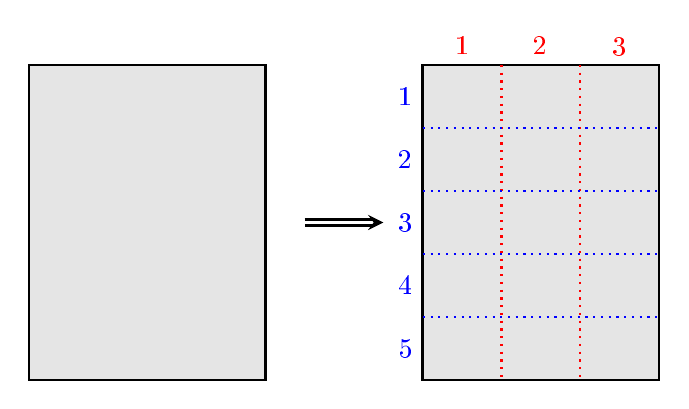
\begin{tikzpicture}
\draw[line width=1pt,fill=black!10] (0,0) rectangle ++(3,-4);
\draw[line width=1pt,double distance=1pt,-stealth] (3.5,-2) -- ++(1,0);
\draw[line width=1pt,fill=black!10] (5,0) rectangle ++(3,-4);
\foreach \x in {1,2}{\draw[dotted,line width=.8pt,red] (5cm+\x cm,0) node[above,xshift=-.5cm] {\x} -- ++(0,-4);}\node[red,above] at (7.5,0) {3};
\foreach \y in {1,...,4}{\draw[dotted,line width=.8pt,blue] (5cm,-.8*\y cm) node[left,yshift=.4cm] {\y} -- ++(3,0);}\node[blue,left] at (5,-3.6) {5};
\end{tikzpicture}}
\\ [10pt]The next task is to assign contents to the cell by typing \textit{trios} with the structure
\begin{itemize}
\item[--]\textbf{(row;column;content)}\item[--]or \textbf{(start row-end row;start column-end column;content)}\item[--]or a combination of both.
\end{itemize}
The available \textbf{contents} are: Z, name, CS, Ar, Ar*, radio, R, Rcov, Rion, Ei, eneg, eaff, O, Tmelt, TmeltC, Tboil, TboilC, eDist, eConfign, eConfignl, d, Cp, kT, ls, lsa, lsb, lsc, lsca, DiscY, DiscC and spectra.
\\ [16pt]Assigning, for instance, \green{(1;1;Z)} will show the atomic number in the first row and in the first column,
\\ [6pt]\pgfPTMcelldesign(1;1;Z)(1 to 2)(1 to 2)
\\ [6pt]while the assignment \green{(1;1-2;Z)} will show the atomic number in the first row and filling the first and second columns,
\\ [6pt]\pgfPTMcelldesign(1;1-2;Z)(1 to 2)(1 to 3)
\\ [10pt]It is also possible to start at a \textit{fraction} of a line or column. If it is intended to start a line at the middle of the first column the value used should be \green{1.5}, which means that the start value is at the half (\textit{0.5}) of the first column (\textit{1}), observing that \textit{1.5} is \textit{0.5} plus \textit{1}:
\\ [6pt]\pgfPTMcelldesign(1;1.5;Z)(1 to 2)(1.5 to 2.5)
\\ [10pt]As in the second example above it is possible to end up in a specified \textit{fraction} of a line or column:
\\ [6pt]\pgfPTMcelldesign(1;1.5-3.5;Z)(1 to 2)(1.5 to 3.5)
\\ [48pt]\tikz{\node[text width=\linewidth-.6666em,fill=green!5!white,draw=green!50!black,rounded corners=2pt] {%
\index{COMMANDS@\textbf{COMMANDS}!\textbackslash pgfPTbuildcell!row, column syntax}%
\textbf{\large The \green{row}, \green{column} \textit{syntax}}
\\ [6pt]Both lines and columns share the same syntax,  where \green{n} is any integer between 1 and the number of rows and \green{f} is the fractional part of any number between 0 and 1:
\begin{itemize}
\item[\bfseries(1)] If only the row number \green{n} is provided the \textit{content} is placed at the row \green{n} .
\item[\bfseries(2)] If the row number \green{n} is provided followed by a \green{dot} and a number \green{f}, the \textit{content} is placed at the fraction \green{f} of the row \green{n}.
\item[\bfseries(3)] If the start row \green{n}\raisebox{-1.5pt}{\small s} and the end row \green{n}\raisebox{-1.5pt}{\small e} are provided separated by a \green{dash}, \ie, \green{n}\raisebox{-1.5pt}{\small s}-\green{n}\raisebox{-1.5pt}{\small e}, the \textit{content} is placed filling all the rows from \green{n}\raisebox{-1.5pt}{\small s} to \green{n}\raisebox{-1.5pt}{\small e}.
    \\ [2pt]\textit{The \green{dot} notation described in }\textbf{(2)} \textit{can be used both on }\green{n}\raisebox{-1.5pt}{\small s} \textit{and } \green{n}\raisebox{-1.5pt}{\small e}.
\item[\bfseries(4)] All of the items above apply to columns in the same way.
\end{itemize}
};}
\subsection{\texorpdfstring{$\maltese$ The cell contents}{The cell contents}}
\makeatletter%
\setbox0=\hbox{\pgfPT@set@econfig[]{[Ar]::3d+1,4s+2}}%
\setbox1=\hbox{\pgfPT@set@econfig[]{[Ar]::4s+2,3d+1}}%
\makeatother%
\begin{itemlist}\hangindent=50pt
\item\textbf{Z} -- the atomic number of the elements.
\item\textbf{name} -- the name of the elements.
\item\textbf{CS} -- the chemical symbol of the elements.
\item\textbf{Ar} -- the relative atomic mass (atomic weight) of the elements.
\item\textbf{Ar*} --the standard relative atomic mass (standard atomic weight) of the elements.
\item\pgfPTMparbox{\textbf{radio} -- radioactivity of the elements. If the element is radioactive the figure \includegraphics[height=6.5pt]{pgfPT_radio_symbol.pdf} is placed in the cell, otherwise nothing is shown.}
\item\pgfPTMparbox{\textbf{R} -- the atomic radius of the elements. The atomic radius shown is the calculated radius and is expressed in picometers.}
\item\pgfPTMparbox{\textbf{Rcov} -- the covalent radius of the elements. The covalent radius shown is for single bonds and is expressed in picometers.}
\item\pgfPTMparbox{\textbf{Rion} -- the ionic radius of the elements. The radius shown is the effective ionic radius in picometers.}
\item\pgfPTMparbox{\textbf{Ei} -- the first ionization energy of the elements, measured in {\large$\mathsf{kJ\cdot mol^{-1}}$}. All data from rutherfordium onwards is predicted.}
\item\textbf{eneg} -- the Pauling electronegativity of the elements.
\item\pgfPTMparbox{\textbf{eaff} -- the electroaffinity (electron affinity) of the elements, measured in {\large$\mathsf{kJ\cdot mol^{-1}}$}. Estimated negative values have been replaced by zero, since the negative ions formed in these cases are always unstable (they may have lifetimes of the order of microseconds to milliseconds, and invariably autodetach after some time).}
\item\textbf{O} -- the common oxidation states of the elements.
\item\textbf{Tmelt} -- the melting point, in Kelvin, of the elements.
\item\textbf{TmeltC} -- the melting point, in degrees Celsius, of the elements.
\item\textbf{Tboil} -- the boiling point, in Kelvin, of the elements.
\item\textbf{TboilC} -- the boiling point, in degrees Celsius, of the elements.
\item\textbf{eDist} -- the electron distribution of the elements.
\item\pgfPTMparbox{\textbf{eConfign} -- the electronic configuration, in increasing n (principal quantum number), of the element, corresponding to the \textit{spectroscopic} order of orbital energies, that is, the reverse of the order in which electrons are removed from a given atom to form positive ions.}
\\ [6pt]\makebox[.1\linewidth][s]{}\begin{minipage}{.9\linewidth}\footnotesize\blue{\textit{\textbf{Note}: the short version of the electronic configuration is used, \ie, [previous noble gas]remaining electrons. For example, for scandium it is: \scalebox{2}{\usebox0}}}\end{minipage}
\item\pgfPTMparbox{\textbf{eConfignl} --  the electronic configuration, in increasing sum of n and {\large$\ell$} (azimuthal quantum number), of the element, following the order based on the Madelung rule.}
\\ [6pt]\makebox[.1\linewidth][s]{}\begin{minipage}{.9\linewidth}\footnotesize\blue{\textit{\textbf{Note}: the short version of the electronic configuration is used, \ie, [previous noble gas]remaining electrons. For example, for scandium it is: \scalebox{2}{\usebox1}}}\end{minipage}
\item\pgfPTMparbox{\textbf{d} -- the density of the elements, in the corresponding physical state, at 25{\large$\mathsf{^oC}$} and 1{\large$\mathsf{\,atm}$}.}
\item\textbf{Cp} -- the specific heat capacity of the elements in {\large$\mathsf{J\cdot mol^{-1}\cdot K^{-1}}$} at 25{\large$\mathsf{^oC}$} and 100{\large$\mathsf{\,kPa}$}.
\item\textbf{kT} -- the thermal conductivity of the elements in {\large$\mathsf{J\cdot m^{-1}\cdot K^{-1}}$} at 25{\large$\mathsf{^oC}$}.
\item\textbf{ls} -- the lattice structure of the elements at 1{\large$\mathsf{\,bar}$} and mostly at 25{\large$\mathsf{^oC}$}.
\item\textbf{lsa} -- the lattice constant {\large$a$} of the elements in picometers at 1{\large$\mathsf{\,bar}$} and mostly at 25{\large$\mathsf{^oC}$}.
\item\pgfPTMparbox{\textbf{lsb} -- the lattice constant {\large$b$} of the eligible elements in picometers at 1{\large$\mathsf{\,bar}$} and mostly at 25{\large$\mathsf{^oC}$}.}
\item\pgfPTMparbox{\textbf{lsc} -- the lattice constant {\large$c$} of the eligible elements in picometers at 1{\large$\mathsf{\,bar}$} and mostly at 25{\large$\mathsf{^oC}$}.}
\item\textbf{lsca} -- the lattice {\large$c/a$} ratio of the eligible elements at 1{\large$\mathsf{\,bar}$} and mostly at 25{\large$\mathsf{^oC}$}.
\item\textbf{DiscY} -- the discovery year of the elements.
\item\textbf{DiscC} -- the discovery country or in, a few cases, region (Middle East or Asia Minor) of the elements.
\item\pgfPTMparbox{\textbf{spectra} -- the emission spectrum of the elements. The spectrum is only shown if available. The spectra are pre-built using the package \href{https://ctan.org/pkg/pgf-spectra}{\large\textsf{pgf-spectra}}\ via the commands:}
    \\ [8pt]\makebox[10pt][s]{}\tikz{\node[text width=\linewidth-.6666em-10pt,fill=green!5!white,draw=green!50!black,rounded corners=2pt] 
    \\ \makebox[3cm][s]{}relative intensity,relative intensity threshold=.375,\textcolor{black!50}{\small\%}
    \\ \makebox[3cm][s]{}brightness=.5,charge=all,Imin=.125,gamma=1}\blue{]}%
    \\ \red{\textbackslash foreach \textbackslash SQ in \{H,He,(...),Bi,Po,Rn,Fr,(...),Es\}}\textcolor{black!50}{\small\% Z=1,2,(...),83,84,86,87,(...),99}
    \\ \makebox[1.6cm][s]{}\red{\{}\textcolor{black!50}{\small\%}
    \\ \makebox[1.6cm][s]{}\blue{\textbackslash pgfspectra[}\red{element=\textbackslash SQ}\blue{]}\textcolor{black!50}{\small\%}
    \\ \makebox[1.6cm][s]{}\red{\}}\textcolor{black!50}{\small\%}};}
\end{itemlist}
\vfill%
\subsection{\texorpdfstring{$\maltese$ Built-in cell styles}{Built-in cell styles}}
There is a set of \textit{built-in} cell styles that could be used for the described purposes:
\index{BUILT-IN@\textbf{BUILT-IN}!
cell styles}%
\vspace{12pt}%
\begin{itemlist}
\item\pdfbookmark[3]{pgfPT2lang}{pgfPT2lang}\pgfPTMparbox{\textbf{pgfPT2lang} --  a cell layout to use with the name in two languages.}
\\ [6pt]\pgfPTpreviewcellstyle[1.6]{pgfPT2lang}\\
\item\pdfbookmark[3]{pgfPT3lang}{pgfPT3lang}\pgfPTMparbox{\textbf{pgfPT3lang} --  a cell layout to use with the name in three languages.}
\\ [6pt]\pgfPTpreviewcellstyle[1.6]{pgfPT3lang}\\
\item\pdfbookmark[3]{pgfPTR}{pgfPTR}\pgfPTMparbox{\textbf{pgfPTR} -- a cell layout to display the atomic radius and its periodic variations (if of course the \red{show periodic variations} key is set to true).}
\\ [6pt]\pgfPTpreviewcellstyle[1.6]{pgfPTR}
\newpage%
\item\pdfbookmark[3]{pgfPTEi}{pgfPTEi}\pgfPTMparbox{\textbf{pgfPTEi} -- a cell layout to display the first ionization energy and its periodic variations (if of course the \red{show periodic variations} key is set to true).}
\\ [6pt]\pgfPTpreviewcellstyle[1.6]{pgfPTEi}\\
\item\pdfbookmark[3]{pgfPTeaff}{pgfPTeaff}\pgfPTMparbox{\textbf{pgfPTeaff} -- a cell layout to display the electron affinity and its periodic variations (if of course the \red{show periodic variations} key is set to true).}
\\ [6pt]\pgfPTpreviewcellstyle[1.6]{pgfPTeaff}\\
\item\pdfbookmark[3]{pgfPTREi}{pgfPTREi}\pgfPTMparbox{\textbf{pgfPTREi} -- a cell layout to display the atomic radius and first ionization energy and their periodic variations (if of course the \red{show periodic variations} key is set to true).}
\\ [6pt]\pgfPTpreviewcellstyle[1.6]{pgfPTREi}\\
\item\pdfbookmark[3]{pgfPTls}{pgfPTls}\pgfPTMparbox{\textbf{pgfPTls} -- a cell layout to display the lattice system.}
\\ [6pt]\pgfPTpreviewcellstyle[1.6]{pgfPTls}
\newpage%
\item\pdfbookmark[3]{pgfPTdisc}{pgfPTdisc}\pgfPTMparbox{\textbf{pgfPTdisc} -- a cell layout to display the discovery country and discovery year.}
\\ [6pt]\pgfPTpreviewcellstyle[1.6]{pgfPTdisc}\\
\end{itemlist}
\endinput
%
\newpage%
\section{\texorpdfstring{Designing color schemes}{Designing color schemes}}
\label{file:DesignCS}%
\hypertarget{colorscheme}{There are three} ways to make a new color scheme:
\begin{itemize}
\item[--]with the command \pgfPTMmacro{pgfPTnewColorScheme}[]
\item[--]using the \textit{script} in the file \mbox{\href{run:pgfPTcolorSchemes.html}{pgfPTcolorSchemes.html}}
\item[--]with the commands provided by the \hyperlink{lib:colorschemes}{colorschemes library} (see the \hyperlink{sec:lib}{libraries section}).
\end{itemize}\ %
\\ [-44pt]\ %
\def\tmpSection{\textcolor{blue!50!black}{\textbackslash pgfPTnewColorScheme}}%
\subsection*{}{{\normalfont\large\bfseries\raisebox{1.25pt}{$\maltese$\ Designing a color scheme with \tmpSection}}%
\label{design:CSscheme}\addcontentsline{toc}{subsection}{\texorpdfstring{$\maltese$\ Designing a color scheme with \tmpSection}{\textbackslash pgfPTnewColorScheme}}%
\\ [4pt]This command provides a way to set the cell background color of each of the 118 elements of the Periodic Table. \textit{If the intention is to set the background color for all of them, it is highly recommended to use the file pgfPTcolorSchemes.html}, unless the trailing color begin at a small atomic number.
\\ [4pt]Despite that, this command can always be used taking into account:
\begin{enumerate}
\item It has the form \pgfPTMmacro{pgfPTnewColorScheme}[trailing color]\blue{\{}\red{name}\blue{\}\{}\red{color list}\blue{\}} where:
\begin{itemize}
\item[--] the first argument (enclosed by square brackets) is optional. If provided, the specified trailing color will be used, otherwise the default color (white) will be used as trailing color.%The trailing color will be used after the last color given in the color list.
\item[--] the second and third arguments are mandatory and specify, respectively, the color scheme name and the color list.
\end{itemize}
\item The \red{name} is any name made up of letters (only the characters a,\myldots,z and A,\myldots,Z).
\item The \red{color list} is a comma-separated list where each entry has the format \red{r/g/b}, representing the red, blue and green values, between 0 and 1, of the color: the first entry of the list will be the background color used in the cell of the element with atomic number 1, the second entry, the background color of the cell of the element with atomic number 2, and so on.
\\ [8pt]\tikz{\node[text width=\linewidth-.6666em,fill=green!5!white,draw=green!50!black,rounded corners=2pt] {%
\textit{If the color list has ten entries, these entries will set the background colors of the elements with atomic numbers from 1 to 10.  For the following atomic numbers, greater than or equal to 11, the \red{trailing color} will be used in the color background}.
};}
\end{enumerate}
\ %
\\ [-44pt]\ %
\def\tmpSection{\textcolor{cyan}{pgfPTcolorSchemes.html}}%
\subsection*{}{{\normalfont\large\bfseries\raisebox{1.25pt}{$\maltese$\ Designing a color scheme with \tmpSection}}%
\label{design:CSscheme}\addcontentsline{toc}{subsection}{\texorpdfstring{$\maltese$\ Designing a color scheme with \tmpSection}{pgfPTcolorSchemes.html}}%
\vfill\makebox[\linewidth][c]{\includegraphics[width=.5\linewidth]{manualfiles/pgfPTcolorSchemes_html_general.pdf}}
\vfill The \href{run:pgfPTcolorSchemes.html}{pgfPTcolorSchemes.html} \textit{designer} is an \textit{html} file with a little \textit{javascript} code to perform the task of building a color scheme to use with the \red{back color scheme} key associated with the \blue{\textbackslash pgfPT} command.
\newpage The Periodic Table of the Elements is displayed on the page and clicking on an element opens a color dialog:
\\ [4pt]\makebox[\linewidth][c]{\includegraphics[width=.7\linewidth]{manualfiles/pgfPTcolorSchemes_html_color.pdf}}
\setbox0=\hbox{\tikz{\draw[btnBorder,fill=black!67] (0,0) rectangle (7.5mm,3mm);}}%
\\ [8pt]Clicking on the {\small Color picker:\hspace{.2ex}}\pgfPTMbtn{\usebox0} button opens a color dialog, where there is the possibility to choose the desired color or manually enter one color using one of the three models available (RGB, HSL or HEX):
\\ [4pt]\makebox[\linewidth][c]{\includegraphics[width=.7\linewidth]{manualfiles/pgfPTcolorSchemes_html_colorPicker.pdf}}
\\ [8pt]After changing the desired colors it is possible to save the color scheme in a file by clicking on \pgfPTMbtn{Write CS to file...}:
\\ [4pt]\makebox[\linewidth][c]{\includegraphics[width=.7\linewidth]{manualfiles/pgfPTcolorSchemes_html_save.pdf}}
\\ [8pt]To use a color scheme saved in a file there are two possible ways:
\begin{itemize}
\item[--]loading the file in the working document via the {\large\textsf{\textbackslash input}} \LaTeX{} command, for instance, {\large\textsf{\textbackslash input\{myCSname.tex\}}}.
\item[--]or by opening the file and copying and pasting its contents into the working document.
\end{itemize}
In either case, the operation can be performed at any location in the document, but before the named color scheme is used.
\\ [4pt]Note that in the previous example there is only one color that has been defined (for hydrogen). In that case, it is useful to set the trailing color in helium by clicking in \pgfPTMbtn{Set trailing color} (which automatically changes to \pgfPTMbtn{Remove trailing color}). After that only the hydrogen and helium are clickable, all the other elements are locked to click:
\\ [4pt]\makebox[\linewidth][c]{\includegraphics[width=.7\linewidth]{manualfiles/pgfPTcolorSchemes_html_trailing.pdf}}
\\ [8pt]Then the saved color scheme will have the optional trailing color and the size will be smaller as only the color codes of the changed elements are stored:
\\ [4pt]\makebox[\linewidth][c]{\includegraphics[width=.7\linewidth]{manualfiles/pgfPTcolorSchemes_html_saveTrailing.pdf}}
\\ [8pt]To remove the trailing color click on the last enabled element (in the  above case helium) and then click on \pgfPTMbtn{Remove trailing color}. After that, all elements can be clicked again.
\\ [8pt]It is also possible to load a color scheme saved to a file by clicking on \pgfPTMbtn{Choose File} and then clicking on \pgfPTMbtn{Update Periodic Table} for the color scheme to take effect:
\\ [4pt]\makebox[\linewidth][c]{\includegraphics[width=.7\linewidth]{manualfiles/pgfPTcolorSchemes_html_load.pdf}}
\\ [4pt]Finally its possible to load a built-in color scheme by choosing a named \textit{pgfPTColorScheme} in the corresponding combo box and then clicking on \pgfPTMbtn{Set selected Color Scheme}:
\\ [4pt]\makebox[\linewidth][c]{\includegraphics[width=.7\linewidth]{manualfiles/pgfPTcolorSchemes_html_set.pdf}}
\\ [20pt]\makebox[\linewidth][c]{\textit{All the operations described are always available}.}
\endinput
%
\newpage\ \vspace{1.5cm}%
\section{Libraries}
In this part the \hypertarget{sec:lib}{library} packages are documented. They provide additional commands to extend the capabilities provided by this package out of the box. The libraries are not loaded by default since many users will not need them.
\\ [1.5cm]%
%\subsection{\texorpdfstring{\ding{224} Color Schemes Library}{colorschemes}}
\subsection*{}{\normalfont\large\bfseries\raisebox{1.25pt}{$\mathbf{\blacktriangleright}$}\ Color Schemes Library}%
\label{command:pgfPTpreviewcell}\addcontentsline{toc}{subsection}{\texorpdfstring{Color Schemes Library}{colorschemes}}%
\index{LIBRARIES@\textbf{\cyan{LIBRARIES}}!colorschemes@\textbf{\red{Color Schemes Library}}}%
%%%%%%%%%%%%%%%%%%%%%%%%%%%%%%%%%%%%%%%%%%%%%%%%%%%%%%%%%%%%
% Color Schemes Library
%%%%%%%%%%%%%%%%%%%%%%%%%%%%%%%%%%%%%%%%%%%%%%%%%%%%%%%%%%%%
\\ [4pt]\pgfPTlib{colorschemes}{This library extends the features provided by the command \bs{\mbox{pgfPTnewColorScheme}}.
It defines a set of commands that automatically generate a new color scheme.
\begin{itemize}
\item\bs{pgfPTGroupColors}\lb\red{name of the new color scheme}\rb\lb\red{list of colors,options}\rb%
\item\bs{pgfPTPeriodColors}\lb\red{name of the new color scheme}\rb\lb\red{list of colors,options}\rb%
\item\bs{pgfPTCScombine}\lp\red{proportion,mode}\rp\lb\red{name of the first color scheme,name of the second color scheme,name of the new color scheme}\rb%
\item\bs{pgfPTCSwrite}\lp\red{filename}\rp\lb\red{list of color schemes names}\rb%
\end{itemize}
Color arguments for this library's commands can use both the base package syntax -- \red{namedColor} or \red{namedColorA!\#\#!namedColorB<!\#\#><!named\myldots>} -- or any color model supported by the \txttt{xcolor} package\footnote{See \textit{Table 3: Supported color models} on page 10 of the documentation of \href{https://ctan.org/pkg/xcolor}{xcolor} v2.14 2022/06/12} using the \textit{special syntax} \red{*[model:values]}, \eg, \red{*[rgb:.5;.2;.3]} or \red{*[cmyk:.5;.2;.3;.3]} or \red{*[HTML:5FA287]}. \textbf{The values for the individual color components of a color specified this way must be separated by semicolons instead of commas}, except for the HTML, Gray and wave color models as explained in the \txttt{xcolor} package.
}% \pgfPTlib
%%%%%%%%%%%%%%%%%%%%%%%%%%%%%%%%%%%%%%%%%%%%%%%%%%%%%%%%%%%%
\def\tmpSectionI{\bs{pgfPTGroupColors}}%
\def\tmpSection{\bs{pgfPTGroupColors}\lp\red{default group color}\rp\lb\red{name of the new color scheme}\rb\lb\red{list of \mbox{colors},options}\rb}%
\subsubsection*{}{\pgfPTMlibsubsubsection{\tmpSection}}%
\label{command:pgfPTGroupColors}\addcontentsline{toc}{subsubsection}{\texorpdfstring{\tmpSectionI{}}{\textbackslash pgfPTGroupColors}}%
\index{LIBRARIES@\textbf{\cyan{LIBRARIES}}!colorschemes@\textbf{\red{Color Schemes Library}}!\tmpSectionI}%
%%%%%%%%%%%%%%%%%%%%%%%%%%%%%%%%%%%%%%%%%%%%%%%%%%%%%%%%%%%%
\\ [10pt]This command \textbf{creates a Color Scheme} with the name \red{name of the new color scheme}. \textbf{Group colors} can be configured in three different ways:
\vspace{4pt}
\begin{itemlist}
\item\textbf{setting the colors one by one}, using the \textit{\red{key=value}} mechanism in the \red{list of colors}. For example:
\mymfbox{\bs{pgfPTGroupColors}\lb\red{name of the new color scheme}\rb\gray{\%}
\\ \lb\red{\textbf{G1=red,G2=red!50,G3=orange,<\myldots>,G18=blue},options}\rb}
\dcyan{\textit{This will set the specified color for each group. If no color is specified for a group, \red{default group color} will be used}.}
\\ [3pt]\blue{\textbf{NOTE}}: \red{default group color} is initially set to white.
\item\textbf{defining a gradient} using the keys \red{left color=<color>}, \red{middle color=<color>} and \red{right color=<color>} as the \red{list of colors}. Note that all the keys are optional, but at least one of them is required. This produces a gradient starting from group 1, with \textit{left color}, to group 18, with \textit{right color}. If the \textit{middle color} key is used then the gradient starts at group 1 with \textit{left color}, goes to the middle position of the groups (between groups 9 and 10) with \textit{middle color} and ends at group 18 with \textit{right color}. For example:
\mymfbox{\bs{pgfPTGroupColors}\lb\red{name of the new color scheme}\rb\gray{\%}
\\ \lb\red{\textbf{left color=red,right color=blue},options}\rb}
\dcyan{\textit{defines a gradient from red (group 1) to blue (group 18)}.}
\item\textbf{defining a custom gradient} as the \red{list of colors} by using the \textit{\red{key=value}} mechanism inside the \red{gradient} key. For example:
\mymfbox{\bs{pgfPTGroupColors}\lb\red{name of the new color scheme}\rb\gray{\%}
\\ \lb\red{\textbf{gradient=\{G1=red,G4=red!50,G18=blue\}},options\rb}}
\dcyan{\textit{defines a gradient from red (group 1) to red!50 (group 4) and to blue (group 18)}.}
\end{itemlist}
\vspace{10pt}
The \red{options} available to this command are:
\vspace{4pt}
\begin{itemlist}
\item\red{H=<color>}, sets the color of the \textit{hydrogen} cell. If not set, group 1's color will be used. If set, the color of the \textit{hydrogen} cell won't be affected by period blending.
\item\red{La=<color>}, sets the color of the \textit{lanthanum} cell. If not set, group 3's color will be used.
\item\red{Lanta=<color>}, sets the color of the \textit{lanthanoids} cells. If not set, \textit{lanthanum}'s color will be used.
\item\red{Ac=<color>}, sets the color of the \textit{actinium} cell. If not set, group 3's color will be used.
\item\red{Actin=<color>}, sets the color of the \textit{actinoids} cells. If not set, \textit{actinium}'s color will be used.
\item\red{period blending=\{color=<color>, percentage=<positive or negative integer>, mode=<add|sub|linear>\}}, performs a \textit{mode} blend over the periods up to the specified percentage with the provided color.
\\ [3pt]\blue{\textbf{NOTES}}:
\begin{itembar}
\item \red{percentage} refers to how much of the color, in total, was mixed over the 7 periods. For example 60\% adds 10\% to each period: P1\raisebox{.8pt}{$\blacktriangleright$}0\% $\rightsquigarrow$ P2\raisebox{.8pt}{$\blacktriangleright$}10\% $\rightsquigarrow$ P3\raisebox{.8pt}{$\blacktriangleright$}20\% $\rightsquigarrow$ \myldots\ $\rightsquigarrow$ P7\raisebox{.8pt}{$\blacktriangleright$}60\%. If the percentage is positive, the mixing is done in descending order (from P1 to P7); if the percentage is negative, the mixing is done in ascending order (from P7 to P1).
\item The \red{mode}'s values are \red{add} for \textit{additive} blending, \red{sub} for \textit{subtractive} blending and \red{linear} for \textit{linear} blending (as in the \texttt{\small xcolor} package).
\item \textbf{If \red{period blending} is used without further options} all the default values are used, so \red{period blending} is equivalent to \red{period blending=\{color=white,percentage=60,mode=linear\}}.
\item None of the keys \red{color}, \red{percentage} and \red{mode} are mandatory. If omitted the default value is used.
\end{itembar}
\end{itemlist}
\newpage%
% examples --------
\pgfPTGroupColors{example}{G1=purple!10,G3=red!10}%
\pgfPTMlibexample{%
\bs{pgfPTGroupColors}\lb\red{example}\rb\lb\red{G1=purple!10,G3=red!10}\rb%
\\ \pgfPTMmacro{pgfPT}[back color scheme=example,show title=false]%
}{%
\scalebox{.425}{\pgfPT[back color scheme=example,show title=false]}%
}% -----
\\ \pgfPTGroupColors[black!10]{example}{G1=purple!10,G3=red!10}%
\pgfPTMlibexample{%
\bs{pgfPTGroupColors}\lp\red{black!10}\rp\lb\red{example}\rb\lb\red{G1=purple!10,G3=red!10}\rb%
\\ \pgfPTMmacro{pgfPT}[back color scheme=example,show title=false]%
}{%
\scalebox{.425}{\pgfPT[back color scheme=example,show title=false]}%
}% -----
\\ \pgfPTGroupColors{example}{G1=*[HTML:FFAAAA],G2=*[HTML:AA3939],G3=*[HTML:FFD1AA],G4=*[HTML:D49A6A],G5=*[HTML:AA6C39],G6=*[HTML:804515],G7=*[HTML:552700],G8=*[HTML:003333],G9=*[HTML:0D4D4D],G10=*[HTML:226666],G11=*[HTML:407F7F],G12=*[HTML:669999],G13=*[HTML:88CC88],G14=*[HTML:55AA55],G15=*[HTML:2D882D],G16=*[HTML:116611],G17=*[HTML:004400],G18=*[HTML:801515]}%
\pgfPTMlibexample{%
\bs{pgfPTGroupColors}\lb\red{example}\rb\lb\red{G1=*[HTML:FFAAAA],G2=*[HTML:AA3939],
G3=*[HTML:FFD1AA],G4=*[HTML:D49A6A],G5=*[HTML:AA6C39],
G6=*[HTML:804515],G7=*[HTML:552700],G8=*[HTML:003333],
G9=*[HTML:0D4D4D],G10=*[HTML:226666],G11=*[HTML:407F7F],
G12=*[HTML:669999],G13=*[HTML:88CC88],G14=*[HTML:55AA55],
G15=*[HTML:2D882D],G16=*[HTML:116611],G17=*[HTML:004400],
G18=*[HTML:801515]
}\rb%
\\ \pgfPTMmacro{pgfPT}[back color scheme=example,show title=false]%
}{%
\scalebox{.425}{\pgfPT[back color scheme=example,show title=false]}%
}% -----
\newpage\pgfPTGroupColors{example}{left color=teal!70,right color=cyan!30}%
\pgfPTMlibexample{%
\bs{pgfPTGroupColors}\lb\red{example}\rb\lb\red{left color=teal!70,right color=cyan!30}\rb%
\\ \pgfPTMmacro{pgfPT}[back color scheme=example,show title=false]%
}{%
\scalebox{.425}{\pgfPT[back color scheme=example,show title=false]}%
}% -----
\vfill\pgfPTGroupColors{example}{left color=teal!70,middle color=yellow!30,right color=cyan!30,La=teal!70!yellow!50,%
Ac=teal!60!yellow!50,Lanta=teal!70!yellow!50!white!50,Actin=teal!60!yellow!50!white!50}%
\pgfPTGroupColors{example}{left color=teal!70,right color=cyan!30,period blending}%
\pgfPTMlibexample{%
\bs{pgfPTGroupColors}\lb\red{example}\rb\lb\red{left color=teal!70,right color=cyan!30,period blending}\rb%
\\ \pgfPTMmacro{pgfPT}[back color scheme=example,show title=false]%
}{%
\scalebox{.425}{\pgfPT[back color scheme=example,show title=false]}%
}% -----
\vfill\pgfPTGroupColors{example}{left color=teal!70,right color=cyan!30,period blending={color=orange!50,percentage=-40}}%
\pgfPTMlibexample{%
\bs{pgfPTGroupColors}\lb\red{example}\rb\lb\red{left color=teal!70,right color=cyan!30,\\ %
period blending=\{color=orange!50,percentage=-40\}}\rb%
\\ \pgfPTMmacro{pgfPT}[back color scheme=example,show title=false]%
}{%
\scalebox{.425}{\pgfPT[back color scheme=example,show title=false]}%
}% -----
\newpage\pgfPTGroupColors{example}{left color=teal!70,right color=cyan!30,period blending={color=orange!50,percentage=-40,mode=add},H={*[cmyk:.071,0,.055,.035]}}%
\pgfPTMlibexample{%
\bs{pgfPTGroupColors}\lb\red{example}\rb\lb\red{left color=teal!70,right color=cyan!30,\\ %
period blending=\{color=orange!50,percentage=-40,mode=add\},\\ %
H=\{*[cmyk:.071,0,.055,.035]\}}\rb%
\\ \pgfPTMmacro{pgfPT}[back color scheme=example,show title=false]%
}{%
\scalebox{.425}{\pgfPT[back color scheme=example,show title=false]}%
}% -----
\pgfPTGroupColors{example}{left color=teal!70,right color=cyan!30,period blending={color=orange!50,percentage=-40,mode=sub},H=*[cmyk:.071;0;.055;.035]}%
\pgfPTMlibexample{%
\bs{pgfPTGroupColors}\lb\red{example}\rb\lb\red{left color=teal!70,right color=cyan!30,\\ %
period blending=\{color=orange!50,percentage=-40,mode=sub\},\\ %
H=*[cmyk:.071;0;.055;.035]}\rb%
\\ \pgfPTMmacro{pgfPT}[back color scheme=example,show title=false]%
}{%
\scalebox{.425}{\pgfPT[back color scheme=example,show title=false]}%
}% -----
\\ \pgfPTGroupColors{example}{left color=teal!70,middle color=yellow!30,right color=cyan!30,La=teal!70!yellow!50,%
Ac=teal!60!yellow!50,Lanta=teal!70!yellow!50!white!50,Actin=teal!60!yellow!50!white!50}%
\pgfPTMlibexample{%
\bs{pgfPTGroupColors}\lb\red{example}\rb\lb\red{left color=teal!70,middle color=yellow!30,right color=cyan!30,%
La=teal!70!yellow!50,Ac=teal!60!yellow!50, Lanta=teal!70!yellow!50!white!50,Actin=teal!60!yellow!50!white!50}\rb%
\\ \pgfPTMmacro{pgfPT}[back color scheme=example,show title=false]%
}{%
\scalebox{.425}{\pgfPT[back color scheme=example,show title=false]}%
}% -----
\newpage%
\pgfPTGroupColors{example}{gradient={G1=teal!50!black,G2=teal,G10=green,G14=orange,G18=blue},period blending={mode=add}}%
\pgfPTMlibexample{%
\bs{pgfPTGroupColors}\lb\red{example}\rb\lb\red{gradient=\{G1=teal!50!black,G2=teal,G10=green,
G14=orange,G18=blue\},period blending=\{mode=add\}}\rb%
\\ \pgfPTMmacro{pgfPT}[back color scheme=example,show title=false]%
}{%
\scalebox{.425}{\pgfPT[back color scheme=example,show title=false]}%
}% -----
\vfill\pgfPTGroupColors{example}{gradient={G3=teal!80!black,G16=teal!80!black,G8=green}}%
\pgfPTMlibexample{%
\bs{pgfPTGroupColors}\lb\red{example}\rb\lb\red{gradient=\{G3=teal!80!black,G16=teal!80!black,
G8=green\}}\rb%
\\ \pgfPTMmacro{pgfPT}[back color scheme=example,show title=false]%
}{%
\scalebox{.425}{\pgfPT[back color scheme=example,show title=false]}%
\\ [6pt]\tikz{\node[text width=\linewidth-.6666em,text justified,font=\small\itshape] {\textbf{Note: the group numbers can be specified in any order and the gradient can start or end in any group}. In this example, the smallest group number is 3 and the greatest is 16, so the gradient is built from group 3 to group 16 and the colors from group 1 to 3 are equal to group 3's color, just like the colors from group 16 to 18 are equal to group 16's color.
};}
}% -----
%%%%%%%%%%%%%%%%%%%%%%%%%%%%%%%%%%%%%%%%%%%%%%%%%%%%%%%%%%%%%
\def\tmpSectionII{\bs{pgfPTPeriodColors}}%
\def\tmpSection{\bs{pgfPTPeriodColors}\lp\red{default period color}\rp\lb\red{name of the new color scheme}\rb\lb\red{list of \mbox{colors},options}\rb}%
\subsubsection*{}{\pgfPTMlibsubsubsection{\tmpSection}}%
\label{command:pgfPTPeriodColors}\addcontentsline{toc}{subsubsection}{\texorpdfstring{\tmpSectionII{}}{\textbackslash pgfPTPeriodColors}}%
\index{LIBRARIES@\textbf{\cyan{LIBRARIES}}!colorschemes@\textbf{\red{Color Schemes Library}}!\tmpSectionII}%
%%%%%%%%%%%%%%%%%%%%%%%%%%%%%%%%%%%%%%%%%%%%%%%%%%%%%%%%%%%%
\\ [10pt]This command \textbf{creates a Color Scheme} with the name \red{name of the new color scheme}. \textbf{Period colors} can be configured in three different ways:
\vspace{4pt}
\begin{itemlist}
\item\textbf{setting the colors one by one}, using the \textit{\red{key=value}} mechanism in the \red{list of colors}. For example:
\mymfbox{\bs{pgfPTPeriodColors}\lb\red{name of the new color scheme}\rb\gray{\%}
\\ \lb\red{\textbf{P1=red,P2=red!50,<\myldots>,P7=blue},options}\rb}
\dcyan{\textit{This will set the specified color for each period. If no color is specified for a period, \red{default period color} will be used}.}
\\ [3pt]\blue{\textbf{NOTE}}: \red{default period color} is initially set to white.
\item\textbf{defining a gradient} using the keys \red{top color=<color>}, \red{middle color=<color>} and \red{bottom color=<color>} as the \red{list of colors}. Note that all the keys are optional, but at least one of them is required. This produces a gradient starting from period 1, with \textit{top color}, to period 7, with \textit{bottom color}. If the \textit{middle color} key is used then the gradient starts at period 1 with \textit{top color}, goes to the middle position of the periods (period 4) with \textit{middle color} and ends at period 7 with \textit{bottom color}. For example:
\mymfbox{\bs{pgfPTPeriodColors}\lb\red{name of the new color scheme}\rb\gray{\%}
\\ \lb\red{\textbf{top color=red,middle color=yellow,bottom color=blue},options}\rb}
\dcyan{\textit{defines a gradient from red (period 1) to yellow (period 4) and from yellow (period 4) to blue (period 7)}.}
\item\textbf{defining a custom gradient} as the \red{list of colors} by using the \textit{\red{key=value}} mechanism inside the \red{gradient} key. For example:
\mymfbox{\bs{pgfPTPeriodColors}\lb\red{name of the new color scheme}\rb\gray{\%}
\\ \lb\red{\textbf{gradient=\{P1=red,P3=red!50,P7=blue\}},options\rb}}
\dcyan{\textit{defines a gradient from red (period 1) to red!50 (period 3) and to blue (period 7)}.}
\end{itemlist}
\vspace{10pt}
The \red{options} available to this command are:
\vspace{4pt}
\begin{itemlist}
\item\red{H=<color>}, sets the color of the \textit{hydrogen} cell. If not set, period 1's color will be used. If set, the color of the \textit{hydrogen} cell won't be affected by group blending.
\item\red{La=<color>}, sets the color of the \textit{lanthanum} cell. If not set, period 6's color will be used.
\item\red{Lanta=<color>}, sets the color of the \textit{lanthanoids} cells. If not set, \textit{lanthanum}'s color will be used.
\item\red{Ac=<color>}, sets the color of the \textit{actinium} cell. If not set, period 7's color will be used.
\item\red{Actin=<color>}, sets the color of the \textit{actinoids} cells. If not set, \textit{actinium}'s color will be used.
\item\red{group blending=\{color=<color>, percentage=<positive or negative integer>, mode=<add|sub|linear>\}}, performs a \textit{mode} blend over the groups up to the specified percentage with the provided color.
\\ [3pt]\blue{\textbf{NOTES}}:
\begin{itembar}
\item \red{percentage} refers to how much of the color, in total, was mixed over the 18 groups. For example 68\% adds 4\% to each period: G1\raisebox{.8pt}{$\blacktriangleright$}0\% $\rightsquigarrow$ G2\raisebox{.8pt}{$\blacktriangleright$}4\% $\rightsquigarrow$ G3\raisebox{.8pt}{$\blacktriangleright$}8\% $\rightsquigarrow$ \myldots\ $\rightsquigarrow$ G18\raisebox{.8pt}{$\blacktriangleright$}68\%. If the percentage is positive, the mixing is done from left to right (from G1 to G18); if the percentage is negative, the mixing is done from right to left (from G18 to G1).
\item The \red{mode}'s values are \red{add} for \textit{additive} blending, \red{sub} for \textit{subtractive} blending and \red{linear} for \textit{linear} blending (as in the \texttt{\small xcolor} package).
\item \textbf{If \red{group blending} is used without further options} all the default values are used, so \red{group blending} is equivalent to \red{group blending=\{color=white,percentage=68,mode=linear\}}.
\item None of the keys \red{color}, \red{percentage} and \red{mode} are mandatory. If omitted the default value is used.
\end{itembar}
\end{itemlist}
\newpage
% examples --------
\pgfPTPeriodColors{example}{P1=*[RGB:86;139;137],P2=*[RGB:49;114;112],P3=*[RGB:23;91;88],P4=*[RGB:5;67;64],P5=*[RGB:35;54;100],P6=*[RGB:62;82;126],P7=*[RGB:101;117;153]}%
\pgfPTMlibexample{%
\bs{pgfPTPeriodColors}\lb\red{example}\rb\lb\red{P1=*[RGB:86;139;137],P2=*[RGB:49;114;112],
P3=*[RGB:23;91;88],P4=*[RGB:5;67;64],P5=*[RGB:35;54;100],
P6=*[RGB:62;82;126],P7=*[RGB:101;117;153]}\rb%
\\ \pgfPTMmacro{pgfPT}[back color scheme=example,show title=false]%
}{%
\scalebox{.425}{\pgfPT[back color scheme=example,show title=false]}%
}% -----
\vfill\pgfPTPeriodColors{example}{top color=*[Hsb:117;.57;.6]}%
\pgfPTMlibexample{%
\bs{pgfPTPeriodColors}\lb\red{example}\rb\lb\red{top color=*[Hsb:117;.57;.6]}\rb%
\\ \pgfPTMmacro{pgfPT}[back color scheme=example,show title=false]%
}{%
\scalebox{.425}{\pgfPT[back color scheme=example,show title=false]}%
}% -----
\vfill\pgfPTPeriodColors{example}{gradient={P1=*[Hsb:117;.57;.6],P5=*[Hsb:178;.57;.45]}}%
\pgfPTMlibexample{%
\bs{pgfPTPeriodColors}\lb\red{example}\rb\lb\red{gradient=\{P1=*[Hsb:117;.57;.6], P5=*[Hsb:178;.57;.45]\}}\rb%
\\ \pgfPTMmacro{pgfPT}[back color scheme=example,show title=false]%
}{%
\scalebox{.425}{\pgfPT[back color scheme=example,show title=false]}%
}% -----
\newpage%
%%%%%%%%%%%%%%%%%%%%%%%%%%%%%%%%%%%%%%%%%%%%%%%%%%%%%%%%%%%%
\def\tmpSectionIII{\bs{pgfPTCScombine}}%
\def\tmpSection{\bs{pgfPTCScombine}\lp\red{prop1:prop2,mode}\rp\lb\red{name of color scheme one,name of color\\ \hfill scheme two,name of the new color scheme}\rb}%
\subsubsection*{}{\pgfPTMlibsubsubsection{\tmpSection}}%
\label{command:pgfPTCScombine}\addcontentsline{toc}{subsubsection}{\texorpdfstring{\tmpSectionIII{}}{\textbackslash pgfPTCScombine}}%
\index{LIBRARIES@\textbf{\cyan{LIBRARIES}}!colorschemes@\textbf{\red{Color Schemes Library}}!\tmpSectionIII}%
%%%%%%%%%%%%%%%%%%%%%%%%%%%%%%%%%%%%%%%%%%%%%%%%%%%%%%%%%%%%
\\ [10pt]This command \textbf{combines two named Color Schemes} and merges the result in a new Color Scheme with \red{name of the new color scheme}.
\\ For example \bs{pgfPTCScombine}\lb\red{myCSA,myCSB,myCSC}\rb\ adds the color scheme \red{myCSA} to the color scheme \red{myCSB} and their sum will be available as the color scheme \red{myCSC}.
\\ [3pt]\blue{\textbf{NOTE}}: if the Color Schemes have different sizes (\ie, different number of colors), the last color from the color scheme that ends first will be used until the other color scheme also ends.
\\ [3pt]The optional parameters \lp\red{prop1:prop2,mode}\rp\ are for controlling how the two Color Schemes are combined:
\vspace{4pt}%
\begin{itemlist}
\item The first parameter -- \red{prop1:prop2} -- controls the proportions used to mix the color schemes: \red{prop1} parts of \red{name of color scheme one} and \red{prop2} parts of \red{name of color} \red{scheme two}.  Both \red{prop1} and \red{prop2} must be integer values between 1 and 999.
\\ [3pt]\blue{\textbf{NOTE}}: default proportion is \red{1:1}.
\\ For example, \red{1:4} \dcyan{\textit{will mix each color in the ratio of 1 to 4, \ie, the nth-color from the first color scheme is used as 1/5 of the mixed color and the nth-color from the second color scheme is used as 4/5 of the mixed color}}.
\item The \red{mode} refers to how the colors are mixed: use \red{add} for \textit{additive} mixing, \red{sub} for \textit{subtractive} mixing and \red{linear} for \textit{linear} mixing (as in the \texttt{\large xcolor} package).
\\ [3pt]\blue{\textbf{NOTE}}: default mode is \red{linear}.
\end{itemlist}
\vspace{4pt}%
% examples --------
\pgfPTPeriodColors{period}{top color=red}%
\pgfPTGroupColors{group}{right color=green}%
\pgfPTCScombine{period,group,mix}%
\pgfPTMlibexample{%
\bs{pgfPTPeriodColors}\lb\red{period}\rb\lb\red{top color=red}\rb%
\\ \bs{pgfPTGroupColors}\lb\red{group}\rb\lb\red{right color=green}\rb%
\\ \bs{pgfPTCScombine}\lb\red{period,group,mix}\rb%
\\ \pgfPTMmacro{pgfPT}[back color scheme=mix,show title=false]%
}{%
\scalebox{.425}{\pgfPT[back color scheme=mix,show title=false]}%
}% -----
\newpage\pgfPTCScombine[sub]{period,group,mix}%
\pgfPTMlibexample{%
\bs{pgfPTCScombine}\lp\red{sub}\rp\lb\red{period,group,mix}\rb%
\\ \pgfPTMmacro{pgfPT}[back color scheme=mix,show title=false]%
}{%
\scalebox{.425}{\pgfPT[back color scheme=mix,show title=false]}%
}% -----
\vfill\pgfPTCScombine[add]{period,group,mix}%
\pgfPTMlibexample{%
\bs{pgfPTCScombine}\lp\red{add}\rp\lb\red{period,group,mix}\rb%
\\ \pgfPTMmacro{pgfPT}[back color scheme=mix,show title=false]%
}{%
\scalebox{.425}{\pgfPT[back color scheme=mix,show title=false]}%
}% -----
\vfill\pgfPTCScombine[3:1]{period,group,mix}%
\pgfPTMlibexample{%
\bs{pgfPTCScombine}\lp\red{3:1}\rp\lb\red{period,group,mix}\rb%
\\ \pgfPTMmacro{pgfPT}[back color scheme=mix,show title=false]%
}{%
\scalebox{.425}{\pgfPT[back color scheme=mix,show title=false]}%
}% -----
\newpage\pgfPTCScombine[3:1,add]{period,group,mix}%
\pgfPTMlibexample{%
\bs{pgfPTCScombine}\lp\red{3:1,add}\rp\lb\red{period,group,mix}\rb%
\\ \pgfPTMmacro{pgfPT}[back color scheme=mix,show title=false]%
}{%
\scalebox{.425}{\pgfPT[back color scheme=mix,show title=false]}%
}% -----
\vfill\pgfPTCScombine[add,2:3]{period,group,mix}%
\pgfPTMlibexample{%
\bs{pgfPTCScombine}\lp\red{add,2:3}\rp\lb\red{period,group,mix}\rb%
\\ \pgfPTMmacro{pgfPT}[back color scheme=mix,show title=false]%
}{%
\scalebox{.425}{\pgfPT[back color scheme=mix,show title=false]}%
}% -----
\vfill\pgfPTCScombine[add]{Soft,group,mix}%
\textit{Built-in color schemes can also be mixed}:
\\ [10pt]\pgfPTMlibexample{%
\bs{pgfPTCScombine}\lp\red{add}\rp\lb\red{Soft,group,mix}\rb%
\\ \pgfPTMmacro{pgfPT}[back color scheme=mix,show title=false]%
}{%
\scalebox{.425}{\pgfPT[back color scheme=mix,show title=false]}%
}% -----
\newpage\pgfPTCScombine[add,3:1]{Soft,PS,mix}%
\pgfPTMlibexample{%
\bs{pgfPTCScombine}\lp\red{add,3:1}\rp\lb\red{Soft,PS,mix}\rb%
\\ \pgfPTMmacro{pgfPT}[back color scheme=mix,show title=false]%
}{%
\scalebox{.425}{\pgfPT[back color scheme=mix,show title=false]}%
}% -----
\\ [4pt]\pgfPTCScombine{Radio,Wikipedia,mix}%
\pgfPTMlibexample{%
\bs{pgfPTCScombine}\lp\red{add}\rp\lb\red{Radio,Wikipedia,mix}\rb%
\\ \pgfPTMmacro{pgfPT}[back color scheme=mix,show title=false]%
}{%
\scalebox{.425}{\pgfPT[back color scheme=mix,show title=false]}%
}% -----
%%%%%%%%%%%%%%%%%%%%%%%%%%%%%%%%%%%%%%%%%%%%%%%%%%%%%%%%%%%%
\def\tmpSectionIV{\bs{pgfPTCSwrite}}%
\def\tmpSection{\bs{pgfPTCSwrite}\lp\red{filename}\rp\lb\red{list of color schemes names}\rb}%
\subsubsection*{}{\pgfPTMlibsubsubsection{\tmpSection}}%
\label{command:pgfPTGroupColors}\addcontentsline{toc}{subsubsection}{\texorpdfstring{\tmpSectionIV{}}{\textbackslash pgfPTCSwrite}}%
\index{LIBRARIES@\textbf{\cyan{LIBRARIES}}!colorschemes@\textbf{\red{Color Schemes Library}}!\tmpSectionIV}%
%%%%%%%%%%%%%%%%%%%%%%%%%%%%%%%%%%%%%%%%%%%%%%%%%%%%%%%%%%%%
\\ [10pt]This command \textbf{writes the provided Color Schemes to a file} for later use without loading this library. It has a mandatory argument, the \red{list of the color schemes names} to be written and an optional argument, the \red{filename}. If no \red{filename} is provided the first name on the \red{list of the color schemes names} is used.
\\ For example, \bs{pgfPTCSwrite}\lp\red{myGroupColors}\rp\lb\red{myGroupGradGreenToRed,myGroupGreens, myGroupGradYellowToRed}\rb, \dcyan{\textit{will create (or overwrite), in the current working directory, a file with name} \texttt{\large myGroupColors.tex} \textit{with the follwing contents}}:
\mymfbox{\textsf{%
\textbackslash pgfPTnewColorScheme\{myGroupGradGreenToRed\}\{0/1/0,\myldots%
\\ \textbackslash pgfPTnewColorScheme\{myGroupGreens\}\{0/1/.1,\myldots%
\\ \textbackslash pgfPTnewColorScheme\{myGroupGradYellowToRed\}\{1/1/0,\myldots}%
}%
After that, it's possible to use \texttt{\large\textbackslash input\{myGroupColors.tex\}}, anywhere in any document (in the same working directory). The named color schemes defined in the loaded file are now available for use as usual:
% examples --------
\\ \pgfPTGroupColors{myGroupGradGreenToRed}{gradient={G1=green!50!black,G18=red!30!black},H=green!40!white}%
\pgfPTGroupColors{myGroupGreens}{gradient={G1=green!50!black,G18=green!50!white},H=green!40!white}%
\pgfPTGroupColors{myGroupGradYellowToRed}{gradient={G1=yellow!50!white,G18=red!30!black},H=yellow!40!white}%
\pgfPTCSwrite[myGroupColors]{myGroupGradGreenToRed,myGroupGreens,myGroupGradYellowToRed}%
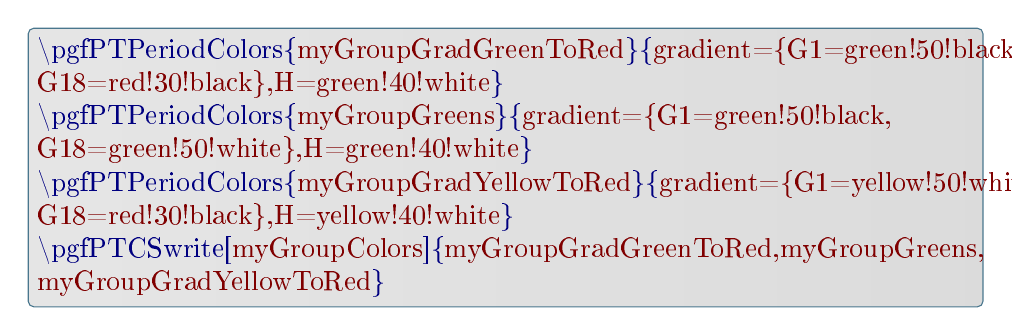
\begin{tikzpicture}%
\node[below right,text width=\textwidth-.6666em,draw=cyan!50!black,rounded corners=2pt,left color=black!10,right color=black!14] (a) at (0,0) {%
\bs{pgfPTPeriodColors}\lb\red{myGroupGradGreenToRed}\rb\lb\red{gradient=\{G1=green!50!black, G18=red!30!black\},H=green!40!white}\rb%
\\ \bs{pgfPTPeriodColors}\lb\red{myGroupGreens}\rb\lb\red{gradient=\{G1=green!50!black, G18=green!50!white\},H=green!40!white}\rb%
\\ \bs{pgfPTPeriodColors}\lb\red{myGroupGradYellowToRed}\rb\lb\red{gradient=\{G1=yellow!50!white, G18=red!30!black\},H=yellow!40!white}\rb%
\\ \bs{pgfPTCSwrite}\lp\red{myGroupColors}\rp\lb\red{myGroupGradGreenToRed,myGroupGreens, myGroupGradYellowToRed}\rb
};%
\end{tikzpicture}%
\\ [4pt]\pgfPTMlibexample{%
\gray{\%\textbackslash usepgfPTlibrary\{colorschemes\}}%
\\ \bs{input}\lb\dcyan{myGroupColors.tex}\rb\gray{\%}%
\\ \pgfPTMmacro{pgfPT}[back color scheme=myGroupGreens,show title=false]%
}{%
\scalebox{.5}{\pgfPT[back color scheme=myGroupGreens,show title=false]}%
}%
%%%%%%%%%%%%%%%%%%%%%%%%%%%%%%%%%%%%%%%%%%%%%%%%%%%%%%%%%%%%
\endinput
%
\newpage%
\section{A few more examples}
%%%%%%%%%%%%%%%%%%%%%%%%%%%%%%%%%%%%%%%%%%%%%%%%%%%%%%%%%%%%
The following examples could be used for students or for any other purposes.
\\ [10pt]\pgfPTMbuildcell(8,3)[(1;1.4-2.8;Z),(1;3;radio),(2-3;1.5-3.5;CS),(4.2;1-3;name), %
(5.4;1-3;Ar),(6.5;1-3;eDist),(7.55-8.95;1-2.25;DiscC),(7.55-8.95;2.25-3.8;DiscY)%
]%
\pgfPTbuildcell(8,3)[%
(1;1.4-2.8;Z),(1;3;radio),%
(2-3;1.5-3.5;CS),(4.2;1-3;name),%
(5.4;1-3;Ar),(6.5;1-3;eDist),%
(7.55-8.95;1-2.25;DiscC),%
(7.55-8.95;2.25-3.8;DiscY)%
]%
\\ [-4pt]\pgfPTMmacrobox{pgfPT}[]%
\\ [10pt]\makebox[\linewidth][c]{\scalebox{.6}{\pgfPT}}%
\vfill%\\ [10pt]
\pgfPTMmacrobox{pgfPT}[eDist color=blue!70!black,Ar precision=2,DiscC font=\string\fontsize{4}{4}\string\selectfont,DiscY font=\string\fontsize{4}{4}\string\selectfont\string\bfseries]
\\ [10pt]\makebox[\linewidth][c]{\scalebox{.6}{\pgfPT[eDist color=blue!70!black,Ar precision=2,DiscC font=\fontsize{4}{4}\selectfont,DiscY font=\fontsize{4}{4}\selectfont\bfseries]}}%
\newpage%
\pgfPTMbuildcell(8,3)[(1;1-2;Z),(1;3;radio),(2-3;1-3;CS),(4;1-3;name),(5;1-2.5;Ar),(5;2.5-3;spectra), %
(7;1-2.5;DiscY),(7;2.5-3;DiscC),(8;1-3;eDist)%
]%
\pgfPTbuildcell(8,3)[%
(1;1-2;Z),(1;3;radio),%
(2-3;1-3;CS),(4;1-3;name),%
(5;1-2.5;Ar),(5;2.5-3;spectra),%
(7;1-2.5;DiscY),(7;2.5-3;DiscC),%
(8;1-3;eDist)%
]%
\\ [-4pt]\pgfPTMmacrobox{pgfPT}[csPS,Ar label=w,background={left color=black!20}]%
\\ [10pt]\makebox[\linewidth][c]{\scalebox{.6}{\pgfPT[csPS,Ar label=w,background={left color=black!20}]}}%
\vfill%
\pgfPTMbuildcell(8,3)[(1;1-3;Z),(1;3;radio),(2-3;1.5-3.5;CS),(4.2;1-3;name),(5.4;1-3;Ar), %
(6.5;1-3;eConfignl),(7.55-8.95;1-2.45;DiscC),(7.55-8.95;2.45-3;DiscY)%
]%
\pgfPTbuildcell(8,3)[%
(1;1-3;Z),(1;3;radio),%
(2-3;1.5-3.5;CS),(4.2;1-3;name),%
(5.4;1-3;Ar),%
(6.5;1-3;eConfignl),%
(7.55-8.95;1-2.45;DiscC),%
(7.55-8.95;2.45-3;DiscY)%
]%
\\ [-4pt]\pgfPTMmacrobox{pgfPT}[eConfignl color=blue!70!black,Ar precision=2,DiscC font=\string\fontsize{4}{4}\string\selectfont,DiscY font=\string\fontsize{4}{4}\string\selectfont\string\bfseries]%
\\ [10pt]\makebox[\linewidth][c]{\scalebox{.6}{\pgfPT[eConfignl color=blue!70!black,Ar precision=2,DiscC font=\fontsize{4}{4}\selectfont,DiscY font=\fontsize{4}{4}\selectfont\bfseries]}}%
\newpage%
\pgfPTresetcell%
\pgfPTPeriodColors{period}{P5=red!20}%
\pgfPTGroupColors{group}{G14=green!20}%
\pgfPTCScombine{period,group,mix}%
\pgfPTMlibexample{%
\textbf{\bs{usepgfPTlibrary}\lb\red{colorschemes}\rb}%
\\ \bs{pgfPTPeriodColors}\lb\red{period}\rb\lb\red{P5=red!20}\rb%
\\ \bs{pgfPTGroupColors}\lb\red{group}\rb\lb\red{G14=green!20}\rb%
\\ \bs{pgfPTCScombine}\lb\red{period,group,mix}\rb%
\\ \pgfPTMmacro{pgfPT}[back color scheme=mix,show title=false]%
}{%
\scalebox{.6}{\pgfPT[back color scheme=mix,show title=false]}%
\\ In the Periodic Table, a row is called a \textbf{\textcolor{red!40}{period}} and a column is called a \textbf{\textcolor{green!40}{group}}.
}% -----
\newpage\ %
\vfill%
\pgfPTbuildcell(8,3)[%
(1;1-3;Z),(1;3;radio),%
(2-3;1.5-3.5;CS),(4.2;1-3;name),%
(5.4;1-3;Ar),%
(6.5;1-3;eDist),%
(7.55-8.95;1-2.45;DiscC),%
(7.55-8.95;2.45-3;DiscY)%
]%
\pgfdeclarelayer{back}\pgfsetlayers{back,main}
\def\grupo[#1][#2] #3{%
\begin{tikzpicture}[inner xsep=0pt]
\node[below left,text width=1.75cm,text centered] (figura) at (0,0) %
{\scalebox{.5}{\pgfPT[show title=false,show label LaAc=true,show legend=false,back color scheme=MNM,%
        font=Roboto-TLF,CS font=\fontfamily{RobotoSlab-TLF}\bfseries\large,eDist color=blue!70!black,%
        DiscC font=\fontsize{4}{4}\selectfont,DiscY font=\fontsize{4}{4}\selectfont\bfseries,%
        name font=\fontseries{l}\fontsize{6pt}{6pt}\selectfont,name color=red!50!black,%
        Ar precision=2,Z list=G#2]}};%
\node[right,text width={\linewidth-2.25cm}] (descricao) at (figura.east) {#1\\ [4pt]#3};
\draw[draw=none,left color=black!20,right color=black!60] (figura.north west) rectangle ++(\linewidth,2pt);
\draw[draw=none,left color=black!20,right color=black!60] (figura.south west) rectangle ++(\linewidth,-2pt);
\begin{pgfonlayer}{back}
\draw[draw=none,left color=black!20,right color=black!60,opacity=.25] (figura.north west) rectangle ([xshift=\linewidth]figura.south west);
\end{pgfonlayer}
\end{tikzpicture}
}%
\tcexemplo[Representative elements: element families]{%
For the \textbf{\textit{representative elements}} (groups \textbf{1}, \textbf{2} and \textbf{13} to \textbf{18}) it is common to speak of families that reflect their common characteristics. So we have \textbf{the families}:
\\ [10pt]\grupo[GROUP \textcolor{blue!50!black}{\textbf{1}}: \textbf{Alkali metals}][1*]
{\red{\raisebox{1.25pt}{$\boldsymbol{\blacktriangleright}$} \textit{lithium, sodium, potassium, rubidium, cesium and francium}.}%
\\ [4.5pt]The atoms of these elements \textbf{have} only \textbf{\textcolor{blue!50!black}{one} valence electron}.%
\vspace{4.5pt}\small\begin{itemlist}
\item They react violently with water to form hydroxides.%
\item They have a silver-gray color, with the exception of cesium, which has a golden hue.%
\end{itemlist}
}%
\\ \grupo[GROUP \textcolor{blue!50!black}{\textbf{2}}: \textbf{Alkaline earth metals}][2]
{\red{\raisebox{1.25pt}{$\boldsymbol{\blacktriangleright}$} \textit{beryllium, magnesium, calcium, strontium, barium and radium}.}%
\\ [4.5pt]The atoms of these elements \textbf{have \textcolor{blue!50!black}{two} valence electrons}.%
\vspace{4.5pt}\small\begin{itemlist}
\item Their oxides remain solid at high temperatures and form alkaline solutions.%
\item They react violently with water to form hydroxides.%
\item When they burn, they have reddish flames, excluding barium, which presents a greenish flame.%
\end{itemlist}
}%
\\ \grupo[GROUP 1\textcolor{blue!50!black}{\textbf{3}}: \textbf{\textit{Boron} group}][13]
{\red{\raisebox{1.25pt}{$\boldsymbol{\blacktriangleright}$} \textit{boron, aluminium, gallium, indium, thallium and nihonium}.}%
\\ [4.5pt]The atoms of these elements \textbf{have \textcolor{blue!50!black}{three} valence electrons}.%
\vspace{4.5pt}\small\begin{itemlist}
\item Boron is a metalloid and the other are metals.%
\item Boron, aluminium, gallium, indium and thallium are often used as p-type silicon dopants.%
\item Aluminium is the third most abundant element in the Earth's crust (7.4\%)%
\end{itemlist}
}%
\\ \grupo[GROUP 1\textcolor{blue!50!black}{\textbf{4}}: \textbf{\textit{Carbon} group}][14]
{\red{\raisebox{1.25pt}{$\boldsymbol{\blacktriangleright}$} \textit{carbon, silicon, germanium, tin, lead and flerovium}.}%
\\ [4.5pt]The atoms of these elements \textbf{have \textcolor{blue!50!black}{four} valence electrons}.%
\vspace{4.5pt}\small\begin{itemlist}
\item Carbon is a non-metal, silicon and germanium are metalloids, and tin and lead are metals.%
\item Silicon and germanium are used in semiconductors.%
\end{itemlist}
}%
\\ \grupo[GROUP 1\textcolor{blue!50!black}{\textbf{5}}: \textbf{Pnictogens}][15]
{\red{\raisebox{1.25pt}{$\boldsymbol{\blacktriangleright}$} \textit{nitrogen, phosphorus, arsenic, antimony, bismuth and moscovium}.}%
\\ [4.5pt]The atoms of these elements \textbf{have \textcolor{blue!50!black}{five} valence electrons}.%
\vspace{4.5pt}\small\begin{itemlist}
\item Nitrogen and phosphorus are non-metals, arsenic and antimony are metalloids and bismuth is a metal.%
\item Phosphorus, arsenic, antimony and bismuth are often used as n-type silicon dopants.%
\item Diatomic nitrogen is the main constituent of the Earth's atmosphere (78\%).%
\end{itemlist}
}%
\\ \grupo[GROUP 1\textcolor{blue!50!black}{\textbf{6}}: \textbf{Chalcogens}][16]
{\red{\raisebox{1.25pt}{$\boldsymbol{\blacktriangleright}$} \textit{oxygen, sulfur, selenium, tellurium, polonium and livermorium}.}%
\\ [4.5pt]The atoms of these elements \textbf{have \textcolor{blue!50!black}{six} valence electrons}.%
\vspace{4.5pt}\small\begin{itemlist}
\item Oxygen, sulfur and selenium are non-metals, tellurium is a metalloid and polonium is a metal.%
\item Diatomic oxygen is the second constituent of the Earth's atmosphere (21\%).%
\end{itemlist}
}%
\\ \grupo[GROUP 1\textcolor{blue!50!black}{\textbf{7}}: \textbf{Halogens}][17]
{\red{\raisebox{1.25pt}{$\boldsymbol{\blacktriangleright}$} \textit{fluorine, chlorine, bromine, iodine, astatine and tennessine}.}%
\\ [4.5pt]The atoms of these elements \textbf{have \textcolor{blue!50!black}{seven} valence electrons}.%
\vspace{4.5pt}\small\begin{itemlist}
\item They are extremely reactive elements, as they are very electronegative.%
\item Fluorine is able to \textit{attack} inert substances, including the heavier noble gas atoms.%
\end{itemlist}
}%
\\ \grupo[GROUP 1\textcolor{blue!50!black}{\textbf{8}}: \textbf{Noble gases}][18]
{\red{\raisebox{1.25pt}{$\boldsymbol{\blacktriangleright}$} \textit{helium, neon, argon, krypton, xenon, radon and oganesson}.}%
\\ [4.5pt]The atoms of these elements have the valence shell fully filled, which corresponds to \textbf{\textcolor{blue!50!black}{eight} valence electrons}, with the exception Helium, which has only one shell and, consequently, has \textbf{two valence electrons}.
\vspace{4.5pt}\small\begin{itemlist}
\item They are extremely inert elements, that is, they do not react with other elements, as they are the most stable elements in Nature.%
\end{itemlist}
}%
}%
\vfill%
\blue{\textit{For the source of this example please see the file} pgf-PeriodicTableManual\_Examples.tex}
\vfill%
\newpage
\mymfbox{%
\textbf{\underline{EXERCISE}:}
\\ [3pt]In the following scheme of the Periodic Table, the positions of some chemical elements are represented by letters:
\\ [3pt]\makebox[\linewidth][c]{\textit{\scriptsize\blue{THE LETTERS DO NOT CORRESPOND TO THE CHEMICAL SYMBOLS OF THE ELEMENTS.}}}
\\ [6pt]\makebox[\linewidth][c]{\pgfPT[Z exercise list={1,2,3,4,9,12,17,18,19,20,25,27,32,34,35,49,54,74,86,87},Z list=spd,%s
                                                           cell size=1.5em,ex={c=blue,f=\bfseries}]}
\\ [6pt]\textbf{Using the letters shown}:
\begin{enumerate}
\item identify group 2 elements of the Periodic Table.%: \hrulefill
\item identify the elements of the 2\raisebox{3pt}{\scriptsize nd} period of the Periodic Table.%: \hrulefill
\item identify group 17 elements of the Periodic Table.%: \hrulefill
\item identify the elements of block s.%: \hrulefill
\item identify the elements of block p.%: \hrulefill
\item identify the elements of block d.%: \hrulefill
\item identify the metallic elements.%: \hrulefill
\item identify the non-metallic elements.%: \hrulefill
\item identify the transition metals.%: \hrulefill
\item identify the alkaline earth metals.%: \hrulefill
\item identify the noble gases.%: \hrulefill
\item tell which element belongs, simultaneously, to the 4\raisebox{3pt}{\scriptsize th} period and to group 14.%\\ [6pt]\makebox[\linewidth][s]{\hrulefill}
\item identify the representative elements that tend to generate positive ions.%:\\ [6pt]\makebox[\linewidth][s]{\hrulefill}
\item indicate an element that forms binegative ions.%: \hrulefill
\item indicate the halogen whose mononegative ion has the largest radius.%: \hrulefill
\item write the chemical formula of the compound formed by the elements \textbf{\blue{F}} and \textbf{\blue{O}}.%\\ [6pt]\makebox[\linewidth][s]{\hrulefill}
\item identify, justifying, the element with the largest atomic radius.%:\\ [6pt]\makebox[\linewidth][s]{\hrulefill}\\ [6pt]\makebox[\linewidth][s]{\hrulefill}
\item identify, justifying, the element with the lowest 1\raisebox{3pt}{\scriptsize st} ionization \mbox{energy}.%:\\ [6pt]\makebox[\linewidth][s]{\hrulefill}\\ [6pt]\makebox[\linewidth][s]{ \hrulefill}
\end{enumerate}
}%
\vfill%
\blue{\textit{For the source of this example please see the file} pgf-PeriodicTableManual\_Examples.tex}
\vfill%
\newpage
\def\xbox{\tikz[baseline=(x.base)]{\node[text width=15pt,text centered,font=\Large,draw,thick,rounded corners=.5pt,inner sep=0pt] (x) {\vbox to 15pt{\vfil\color{gray}x\vfil}};}}%
\def\obox{\tikz[baseline=(x.base)]{\node[text width=15pt,text centered,draw,thick,rounded corners=.5pt,inner sep=0pt] (x) {\vbox to 15pt{\vfil\color{gray}$\bigcirc$\vfil}};}}%
\def\dbox{\tikz[baseline=(x.base)]{\node[text width=15pt,text centered,font=\Large,draw,thick,rounded corners=.5pt,inner sep=0pt] (x) {\vbox to 15pt{\vfil\color{gray}$\Delta$\vfil}};}}%
\mymfbox{%
\textbf{\underline{EXERCISE}:}
\\ [3pt]Using the following notation,
\begin{itemize}
\item[\xbox] for the elements in the gaseous state (NTP),
\item[\obox] for the elements in the liquid state (NTP) and
\item[\dbox] for the synthetic elements,
\end{itemize}
fill in the following Periodic Table:
\\ [10pt]\makebox[\linewidth][c]{\scalebox{.6}{\pgfPT[only cells]}}
}
\vspace{15pt}%
\blue{\textit{For the source of this example please see the file} pgf-PeriodicTableManual\_Examples.tex}%
\endinput
%
\newpage\small%
\printindex%
\end{document}
